\documentclass[11pt, a4paper]{article}
\usepackage[utf8]{inputenc}
\usepackage[ngerman]{babel}
\usepackage[T1]{fontenc}
\usepackage{amsmath}
\usepackage{amsfonts}
\usepackage{amssymb}
\usepackage[dvipsnames]{xcolor}
\usepackage{hyperref}
\usepackage{cleveref}
\usepackage{enumitem}
\usepackage{geometry}
\usepackage{adjustbox}
\usepackage{graphicx}
\graphicspath{{Images/}}


\title{Software Engineering}
\author{Zusammenfassung}
\date{SoSe 2024}

\begin{document}
\maketitle

\tableofcontents
\newpage


% --- START DES EIGENTLICHEN INHALTS -------------------------------------------------


\section{Einführung} % --- Einführung ------------------------------------------------------------------------------------

\subsection{Ziele des Software Engineering}

\begin{enumerate}
    \item \textbf{Qualität}:
    \begin{itemize}
        \item Zuverlässigkeit
        \item Wartbarkeit
        \item Benutzerfreundlichkeit
        \item Performanz
        \item Effizienz
    \end{itemize}

    \item \textbf{Kosten}:
    \begin{itemize}
        \item Entwicklungskosten
        \item Wartungskosten
        \item Vertriebskosten
    \end{itemize}

    \item \textbf{Zeit}:
    \begin{itemize}
        \item Verkürzung der Entwicklungszeit durch mehr Personal
        \item Spezialisten und motivierte Teams
    \end{itemize}

    \item \textbf{Wirtschaftlichkeit}:
    \begin{itemize}
        \item Umsatz und Kosteneinsparung durch effiziente Softwarelösungen
    \end{itemize}
\end{enumerate}

\newpage

\section{Ethik} % --- Ethik ------------------------------------------------------------------------------------

\subsection{Internationale Organisationen}

\begin{itemize}
    \item ACM(Association for Computing Machinery)
    \item IEEE (Institute of Electrical and Electronic Engineers)
    \item British Computer Society
\end{itemize}

“Software Engineering Code of Ethics and Professional Practice”

\footnotesize \url{https://ethics.acm.org/code-of-ethics/software-engineering-code/}

\subsection{8 Prinzipien des ACM/IEEE Code of Ethics}

\begin{enumerate}
    \item \textbf{Public}:
    \begin{itemize}
        \item Handeln im öffentlichen Interessen
        \item Volle Verantwortung für seinen Code übernehmen
        \item Genehmigen Sie Software nur, wenn sie sicher ist, die Spezifikationen erfüllt, 
        geeignete Tests besteht und die Lebensqualität nicht beeinträchtigt, 
        die Privatsphäre nicht verletzt und die Umwelt nicht schädigt
    \end{itemize}

    \item \textbf{Client and Employer}:
    \begin{itemize}
        \item Interessen von Kunden und Arbeitgebern wahren
    \end{itemize}

    \item \textbf{Product}:
    \begin{itemize}
        \item Höchste professionelle Standards für Produkte sicherstellen
    \end{itemize}

    \item \textbf{Judgement}:
    \begin{itemize}
        \item Integrität und Unabhängigkeit im beruflichen Urteil bewahren
    \end{itemize}

    \item \textbf{Management}:
    \begin{itemize}
        \item Ethisches Management von Softwareentwicklung und -wartung
    \end{itemize}

    \item \textbf{Profession}:
    \begin{itemize}
        \item Integrität und Reputation des Berufsstandes fördern
    \end{itemize}

    \item \textbf{Colleagues}:
    \begin{itemize}
        \item Fair und unterstützend gegenüber Kollegen sein
    \end{itemize}

    \item \textbf{Self}:
    \begin{itemize}
        \item Lebenslanges Lernen und ethische Praxis fördern
    \end{itemize}
\end{enumerate}

\subsection{Ethikfragen im Software Engineering}

\begin{itemize}
    \item Ist die Verbreitung von Viren/Trojanern ein ethisches Problem?
    \item Ist fehlerhafter Code ein ethisches Problem?
    \item Ist schwer lesbarer Code ein ethisches Problem?
    \item Ist das Unterschätzen der Schwierigkeit eines SW-Projekts ein ethisches Problem?
    \item Ist das Unterschätzen der Kosten eines Softwareprojekts ein ethisches Problem?
    \item Ist es ein ethisches Problem, nicht immer die neuesten Technologien zu nutzen?
\end{itemize}

\newpage

\section{Projektphasen} % --- Projektphasen ------------------------------------------------------------------------------------

\subsection{Wie kommt man zu einem Projekt?}

\begin{figure}[h]
    \centering
    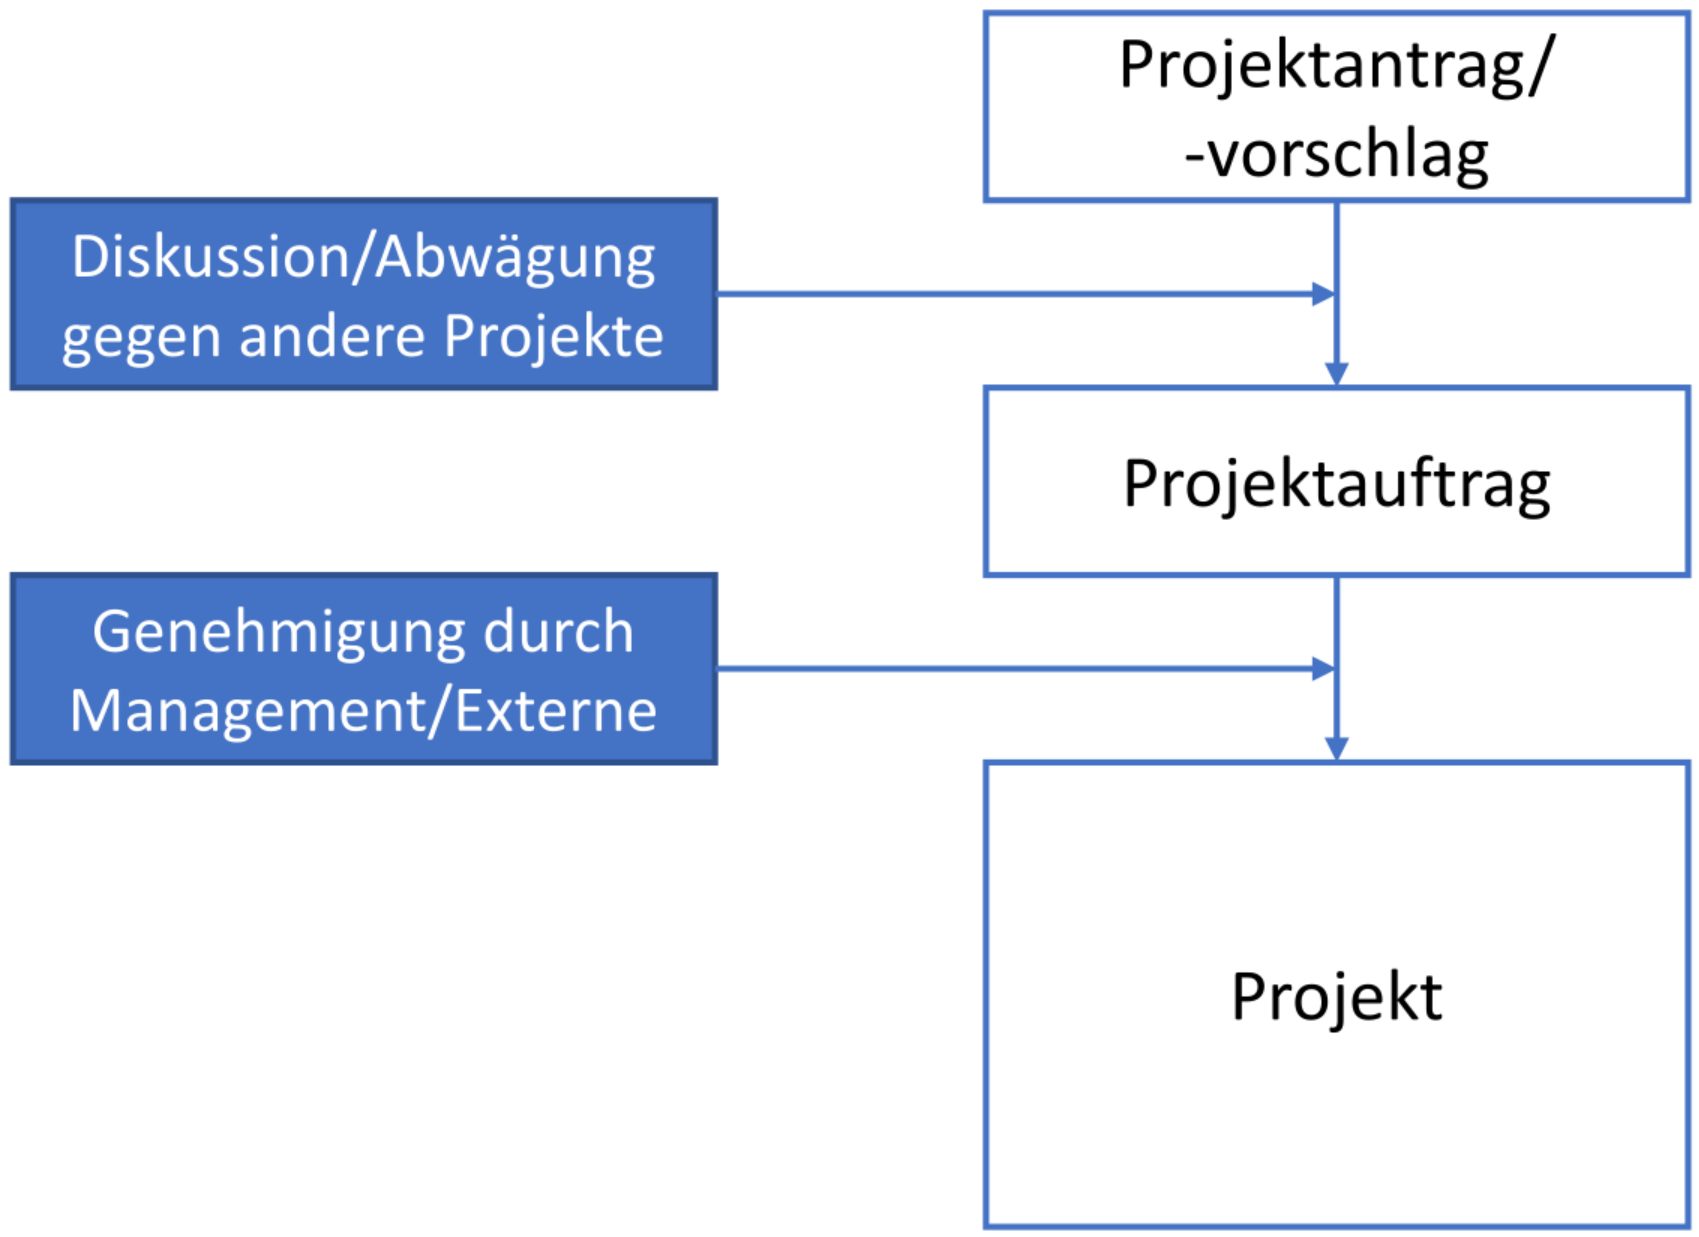
\includegraphics[width=0.75\textwidth]{Projektphasen-00}
    \caption{Projektantrag Ablauf}
    \label{fig:Projektphasen-00}
\end{figure}



\subsubsection{Projektantrag}

\begin{itemize}
    \item \textbf{Ziel:} Darlegung der Projektidee
    \item \textbf{Inhalte:}
    \begin{itemize}
        \item Ausgangslage (Status quo, welches Problem wollen wir lösen?)
        \item Ziele
        \item Kosten/Nutzen
        \item Organisation
    \end{itemize}
    \item \textbf{Ausprägungen:}
    \begin{itemize}
        \item Interne Projekte
        \item öffentlich geförderte Projekte
    \end{itemize}
\end{itemize}

\newpage

\subsubsection{Projektauftrag}

Offizieller Startschuss für das Projekt. Projektauftrag ist das erste Projektdokument. \\
\textbf{!!!Kein Projekt ohne Projektauftrag!!!}

\begin{itemize}
    \item \textbf{Inhalte:} 
    \begin{itemize}
        \item Projektbezeichnung
        \item Auftraggeber
        \item Beginn und Ende
        \item Kurzbeschreibung
        \item Unternehmensbedarf
        \item Ziele
        \item Projektergebnisse
        \item Budget
        \item Projektleiter
        \item Team
        \item Annahmen
        \item Beschränkungen
        \item Terminvorgaben
    \end{itemize}
\end{itemize}

Unternehmen haben sehr unterschiedliche Handhabung im Umgang mit Projektantrag und Projektauftrag. 
Er hängt von Organisationsstruktur und Kultur des Unternehmens ab.
Bei mittelgroßen/großen Unternehmen gibt es normalerweise Vorlagen für den Projektauftrag!

\subsection{Phasen eines Softwareprojekts}

\begin{figure}[h]
    \centering
    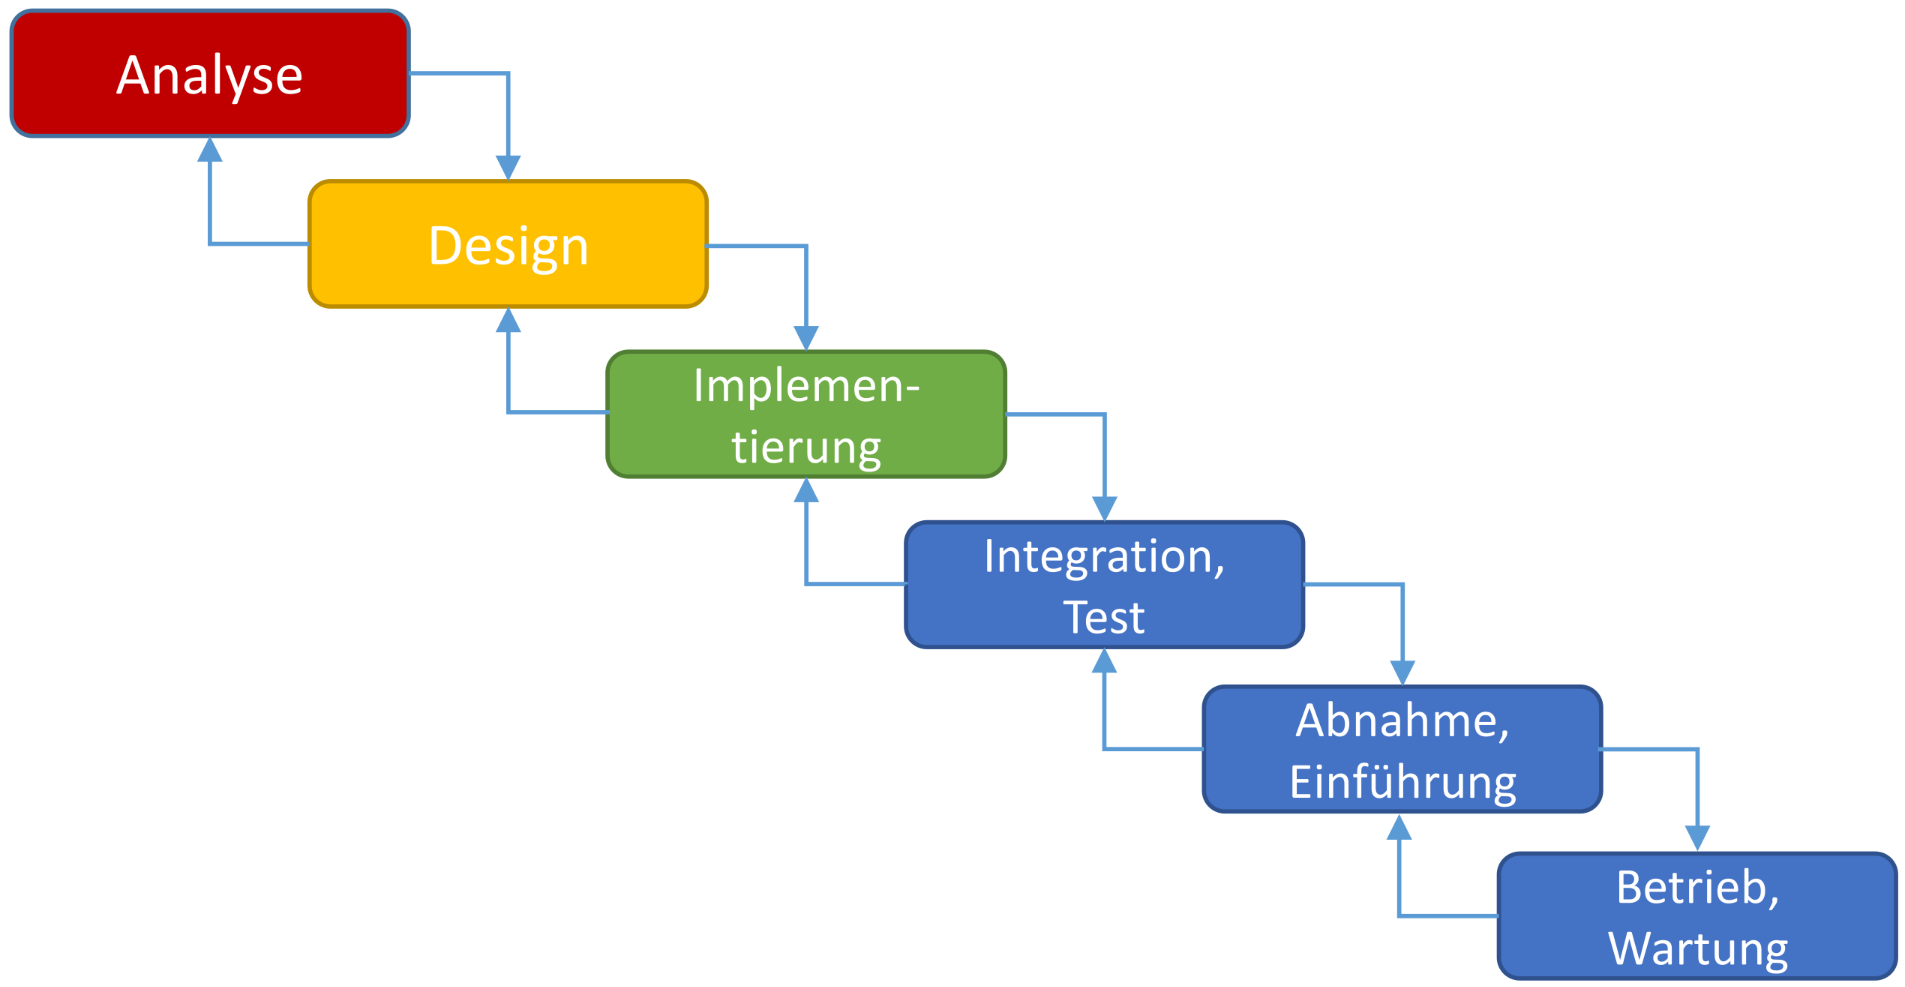
\includegraphics[width=0.75\textwidth]{Projektphasen-01}
    \caption{Projektphasen Ablauf}
    \label{fig:Projektphasen-01}
\end{figure}

\subsubsection*{Analyse}

\begin{itemize}
    \item Aufstellen von Leistungen, Einschränkungen und Zielen des Systems
    \item In Zusammenarbeit mit den Systembenutzern/dem Kunden
    \item Anschließend detailliertere Beschreibung und Definition
    \item Ergebnis dient als Systemspezifikation
\end{itemize}

\subsubsection*{Design (Entwurf)}

\begin{itemize}
    \item Anforderungen werden in Hard- oder Softwaresysteme aufgeteilt
    \item Dazu wird übergeordnete Systemarchitektur festgelegt
    \item Beim Software-Design geht es um Erkennen und Beschreiben:
    \begin{itemize}
        \item Der grundlegenden (abstrakten) Softwaresysteme und
        \item Deren Beziehung zueinander
    \end{itemize}
\end{itemize}

\subsubsection*{Implementierung (und Modultests)}

\begin{itemize}
    \item Umsetzung des Softwareentwurfs durch Programme oder Programmeinheiten
    \item Testen der Module auf Einhaltung Ihrer Spezifikation
\end{itemize}

\subsubsection*{Integration, Test}

\begin{itemize}
    \item Zusammenführung/Integration einzelner Programme oder Programmeinheiten
    \item Test des “Ganzen” auf Einhaltung der Anforderungen
    \item Auslieferung an Kunden
\end{itemize}

\subsubsection*{Abnahme, Einführung}

\begin{itemize}
    \item Abnahmetests in mehreren Stufen
    \begin{itemize}
        \item Technische Tests
        \item Last-/Performancetests
        \item Fachliche Tests
        \item User-Acceptance Tests, …
    \end{itemize}
    \item Auslieferung an den Kunden
    \item Ggf. Anwenderschulungen, Informationsmaßnahmen bis hin zu Marketing für die neue Software
\end{itemize}

\subsubsection*{Betrieb, Wartung}

\begin{itemize}
    \item Längste Phase im Software-Lifecycle
    \item System wird installiert und zur Nutzung freigegeben
    \item Elemente der Wartung:
    \begin{itemize}
        \item Beheben von Fehlern
        \item Verbesserung der Implementierung von Systemeinheiten
        \item Verbesserung des Systems, falls neue Anforderungen entstehen
    \end{itemize}
    \item Teil der Wartung häufig noch in Projektkosten enthalten
    \item Später Wartungsverträge
\end{itemize}

\subsection{Allgemeine Hinweise zu den Projektphasen}

\begin{itemize}
    \item Phasen nicht notwendigerweise sequentiell
    \item Tätigkeiten innerhalb der Phasen erfordern verschiedene Qualifikationen
    \item ABER: nicht immer ist (vollständige) Durchführung aller Phase sinnvoll
    \item Tätigkeiten müssen koordiniert werden → Projektmanagement
    \item Softwareprojekte laufen immer in Teams ab (sowohl innerhalb des Unternehmens als auch mit Kooperationspartnern/Kunden)
\end{itemize}

\textbf{$ \rightarrow $ Kommunikation innerhalb des Teams und zwischen Team und Kunden ist extrem wichtig}

\subsection{Dokumente (Artefakte) pro Phase}

Jede Phase bringt Dokumente (Artefakte) hervor, die Input für die folgende Phase sind

\begin{figure}[h]
    \centering
    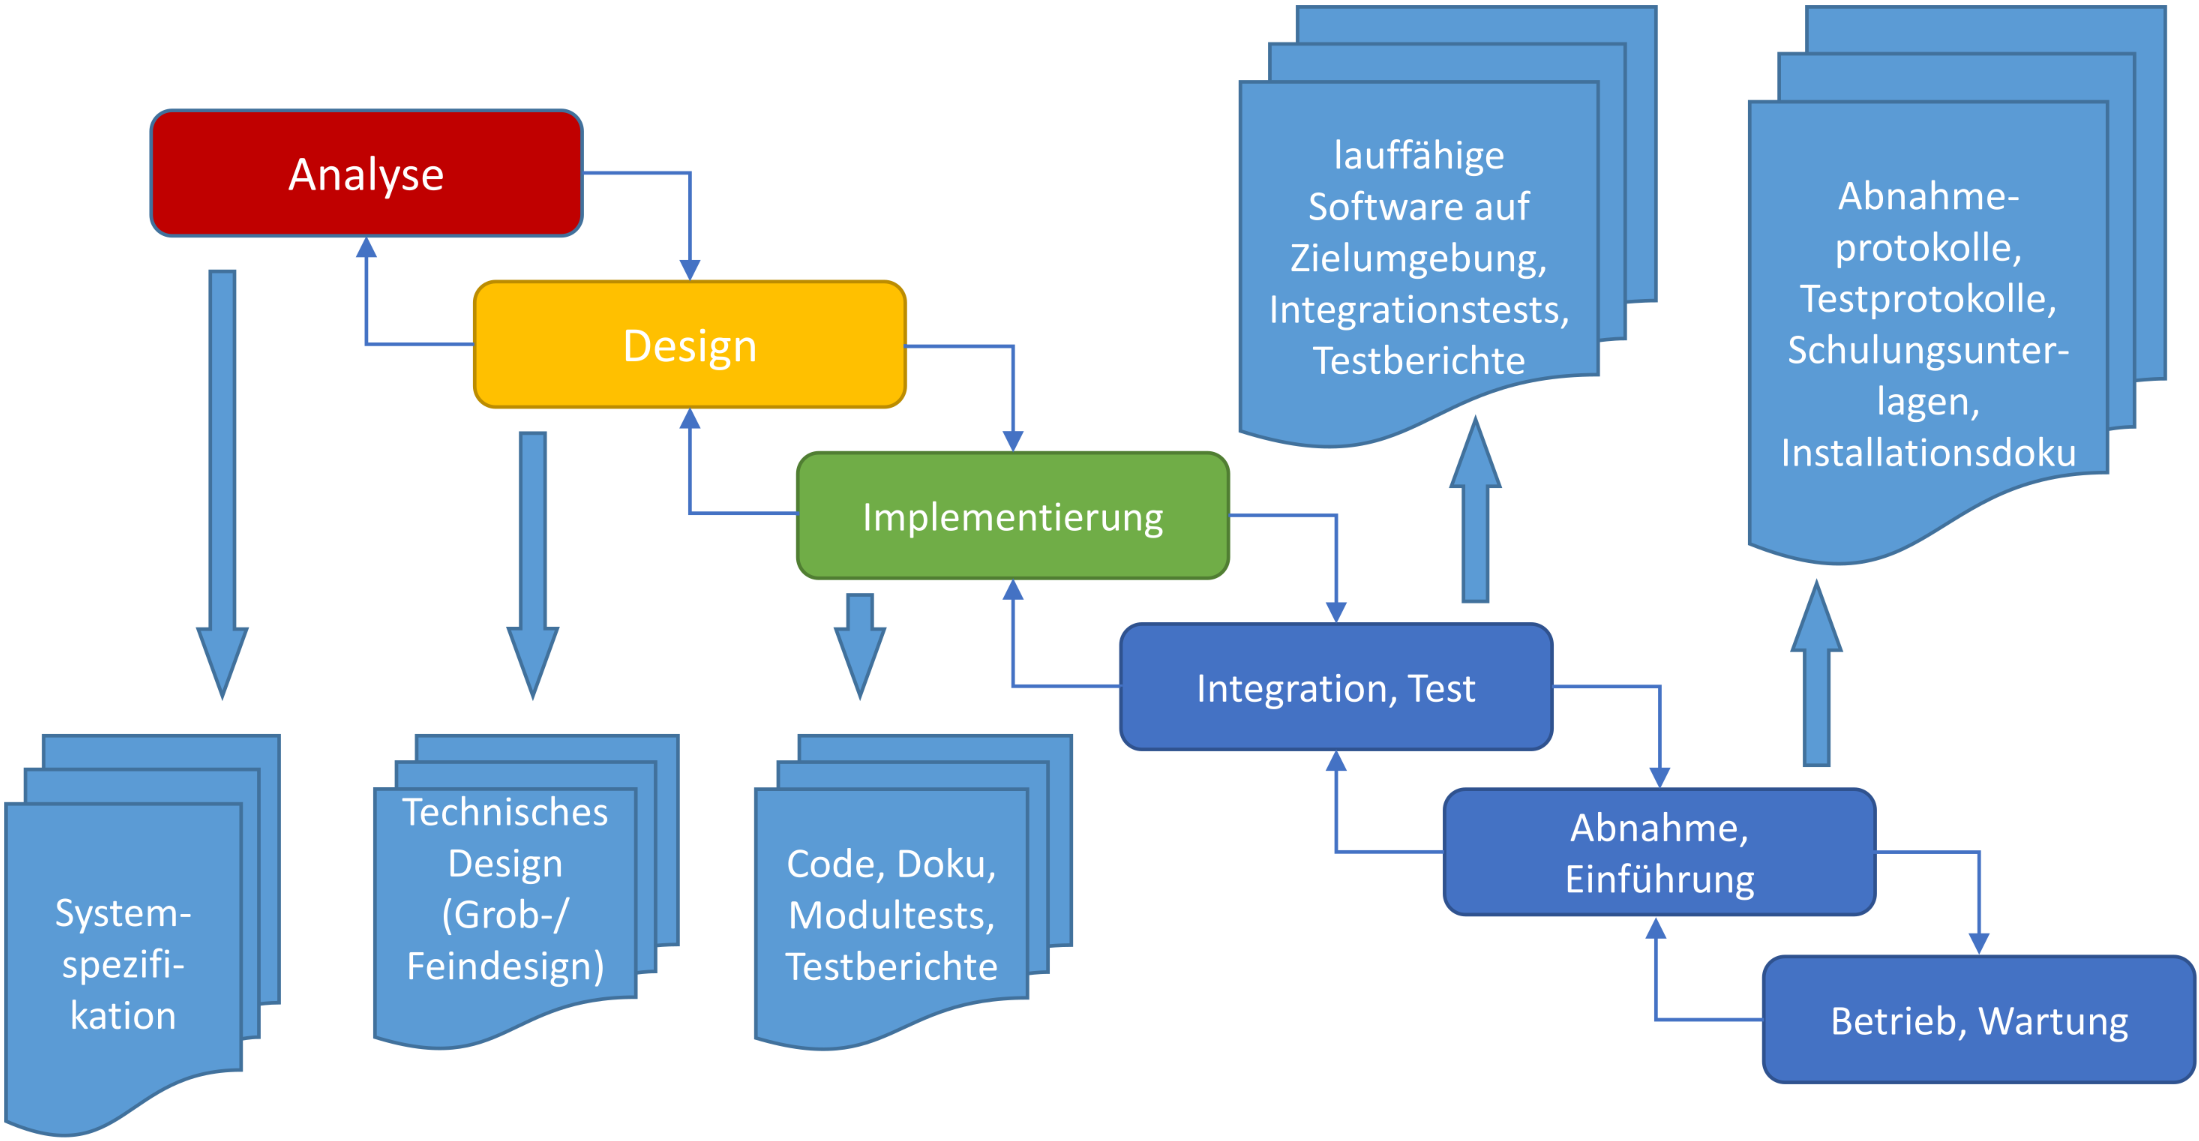
\includegraphics[width=0.75\textwidth]{Projektphasen-02}
    \caption{Dokumente der einzelnen Phasen}
    \label{fig:Projektphasen-02}
\end{figure}

\newpage

\section{Requirements Engineering (Anforderungsanalyse)} % --- Requirements Engineering ------------------------------------------------------------------------------------

\subsection{Überblick und Bedeutung}

\subsubsection*{Definition}

\begin{itemize}
    \item Requirements Engineering ist der Prozess des Herausfindens, Analysierens, Dokumentierens und Überprüfens der Anforderungen an ein System
    \item \textbf{Ziel:} Sicherstellen, dass alle relevanten Anforderungen bekannt und verstanden sind, und dass Stakeholder diesen zustimmen
\end{itemize}


\subsubsection*{Bedeutung der Analysephase}

\begin{itemize}
    \item Fehler in der Analysephase führen zu hohen Kosten und Verzögerungen
    \item 60\% der Softwareprojekte scheitern aufgrund von Analysefehlern
    \item 50\% der Ausfälle im industriellen Sektor sind auf Software-Fehler zurückzuführen
\end{itemize}

\textbf{Grundsatz:} \textit{Frühzeitig Fehlererkennung/-behebung spart Zeit, Kosten, Ärger}

\subsection{Hauptaufgaben}

\subsubsection*{Anforderungen ermitteln}

\begin{itemize}
    \item Systemkontext festlegen
    \item Anforderungen von Stakeholdern sammeln
\end{itemize}

\subsubsection*{Anforderungen dokumentieren}

\begin{itemize}
    \item Beschreibung der Anforderungen in Lasten- und Pflichtenheft
\end{itemize}

\subsubsection*{Anforderungen prüfen und abstimmen}

\begin{itemize}
    \item Überprüfung der Anforderungen auf Vollständigkeit, Konsistenz und Eindeutigkeit
    \item Stakeholder-Review und formale Abnahme
\end{itemize}

\subsubsection*{Anforderungen verwalten}

\begin{itemize}
    \item Änderungen nachverfolgen
    \item Versionierung der Anforderungen
\end{itemize}

\newpage


\subsection{Requirement Dokumente nach IEEE 830-1998}

\subsubsection*{1. Einleitung}

\begin{enumerate}[label=(\alph*)]
    \item Zielsetzung (Vision)
    \item Produktziele
    \item Definitionen, Akronyme, Abkürzungen
    \item Referenzen
    \item Überblick
\end{enumerate}

\subsubsection*{2. Übersichtsbeschreibung}

\begin{enumerate}[label=(\alph*)]
    \item Produkt-Umgebung
    \item Produkt-Funktionen
    \item Benutzer-Eigenschaften
    \item Restriktionen
    \item Annahmen und Abhängigkeiten
\end{enumerate}

\subsubsection*{3. Spezifische Anforderungen}

\begin{enumerate}[label=(\alph*)]
    \item Externe Schnittstellenanforderungen
    \item Funktionale Anforderungen
    \item Leistungsanforderungen
    \item Entwurfsrestriktionen
    \item Eigenschaften des Softwaresystems
    \item Andere Anforderungen
\end{enumerate}

\subsection{Visionen, Ziele und Rahmenbedingungen}

Bevor die Anforderungen und Rahmenbedingungen aufgenommen werden, sollten Visionen und Ziele formuliert werden.

\subsubsection{Visionen}

\begin{itemize}
    \item beschreibt, \textbf{was} erreicht werden soll, aber \textbf{nicht wie}
    \item hat \textbf{geringe Detailtiefe}; dient als \textbf{Leitgedanke}
    \item wird im Rahmen eines Projektauftrags formuliert, der genehmigt werden muss
\end{itemize}

\subsubsection*{Beispiele:}

\textbf{Vision für ein Türsteuergerät für einen Fensterheber:} \\
/V20/ \textit{Die Fensterheberkomponente soll das komfortable Heben und Senken der Seitenfenster eines Fahrzeugs ermöglichen.} 
\\ 
\textbf{Vision für eine Kundendatenbank:} \\
/V20/ \textit{Die Kundendatenbank soll als single point of truth alle Stammdaten der Kunden enthalten.}

\newpage

\subsubsection{Ziele}

Ausgehend von einer Vision dienen Ziele dazu, die \textbf{Vision} zu \textbf{verfeinern} und zu \textbf{operationalisieren}


\subsubsection*{Beispiel: Ziel für den Fensterheber}

\textbf{Vision für ein Türsteuergerät für einen Fensterheber:} \\
/Z20/ \textit{Die erwarteten Stückzahlen betragen 20.000 Einheiten p.a.} 

\subsubsection*{Regeln zur Zielformulierung:}

\begin{enumerate}
    \item Kurz und prägnant formulieren
    \item Aktivformulierung
    \item Überprüfbare und realistische Ziele formulieren
    \item Nicht überprüfbare Ziele verfeinern
    \item Mehrwert eines Ziels hervorheben
    \item Begründung für das Ziel liefern
    \item Keine Lösungsansätze formulieren
\end{enumerate}

\subsubsection*{Eigenschaften von Zielen:}

\begin{itemize}
    \item vollständig
    \item korrekt
    \item konsistent gegenüber anderen Zielen und in sich konsistent
    \item testbar
    \item verständlich für alle Stakeholder
    \item umsetzbar/realisierbar
    \item notwendig
    \item eindeutig und positiv formuliert
\end{itemize}

\subsubsection{Rahmenbedingungen}

Legt organisatorische und technische Restriktionen für das Softwaresystem \\bzw. den Entwicklungsprozess fest.

\begin{itemize}
    \item \textbf{Organisatorische Rahmenbedingungen:}
    \begin{itemize}
        \item Anwendungsbereiche (z.B. Textverarbeitung im Büro)
        \item Zielgruppen (z.B. Sekretärinnen, Schreibkräfte)
        \item Betriebsbedingungen (z.B. Büroumgebung, mobiler Einsatz)
    \end{itemize}
    \item \textbf{Technische Rahmenbedingungen:}
    \begin{itemize}
        \item Technische Produktumgebung
        \item Anforderungen an die Entwicklungsumgebung
    \end{itemize}
\end{itemize}

\newpage


\subsection{Anforderungen}


"Anforderungen legen fest, was man von einem Softwaresystem als Eigenschaften erwartet"

\textit{- Helmut Balzert}

\subsubsection{Funktionale Anforderungen}

\begin{itemize}
    \item Beschreiben, was ein System tun soll (Dienste, Reaktionen auf Eingaben, Verhalten)
\end{itemize}

\subsubsection{Nicht-funktionale Anforderungen}

\begin{itemize}
    \item Beschränkungen
    \item Beziehen sich eher auf das Gesamtsystem als auf einzelne Dienste
\end{itemize}

\subsubsection*{Beispiele: Nicht-funktionale Anforderungen}

\subsubsection*{Technische Anforderungen}
\begin{itemize}
    \item Portierbarkeit
    \item Schnittstellen
\end{itemize}

\subsubsection*{Qualitäts Anforderungen}
\begin{itemize}
    \item Wartbarkeit
    \item Effizienz
    \item Zuverlässigkeit
    \item Änderbarkeit
\end{itemize}

\subsubsection*{Unternehmensanforderungen}
\begin{itemize}
    \item Lieferanforderungen
    \item Vorgehensanforderungen
\end{itemize}

\subsubsection*{Ethische Anforderungen}
\begin{itemize}
    \item \textit{Siehe Kapitel 2.}
\end{itemize}

\subsubsection*{Rechtlich-vertragliche Anforderungen}
\begin{itemize}
    \item Sicherheit
    \item Datenschutz
    \item Gesetze
\end{itemize}

\newpage


\subsection{Stakeholder}

$ \rightarrow $ Jemand der Einfluss auf die Anforderungen hat, da er vom System betroffen ist.

\textbf{"Systembetroffener"}

\begin{itemize}
    \item Sind Quellen für Anforderungen
    \item Übersehen eines Stakeholders führt zu lückenhaften Anforderungen
\end{itemize}

\textbf{Zum Beispiel:} Kunden, Mitarbeiter, Zulieferer, Eigentümer, ...

\subsubsection{Stakeholderliste}

\begin{figure}[h]
    \centering
    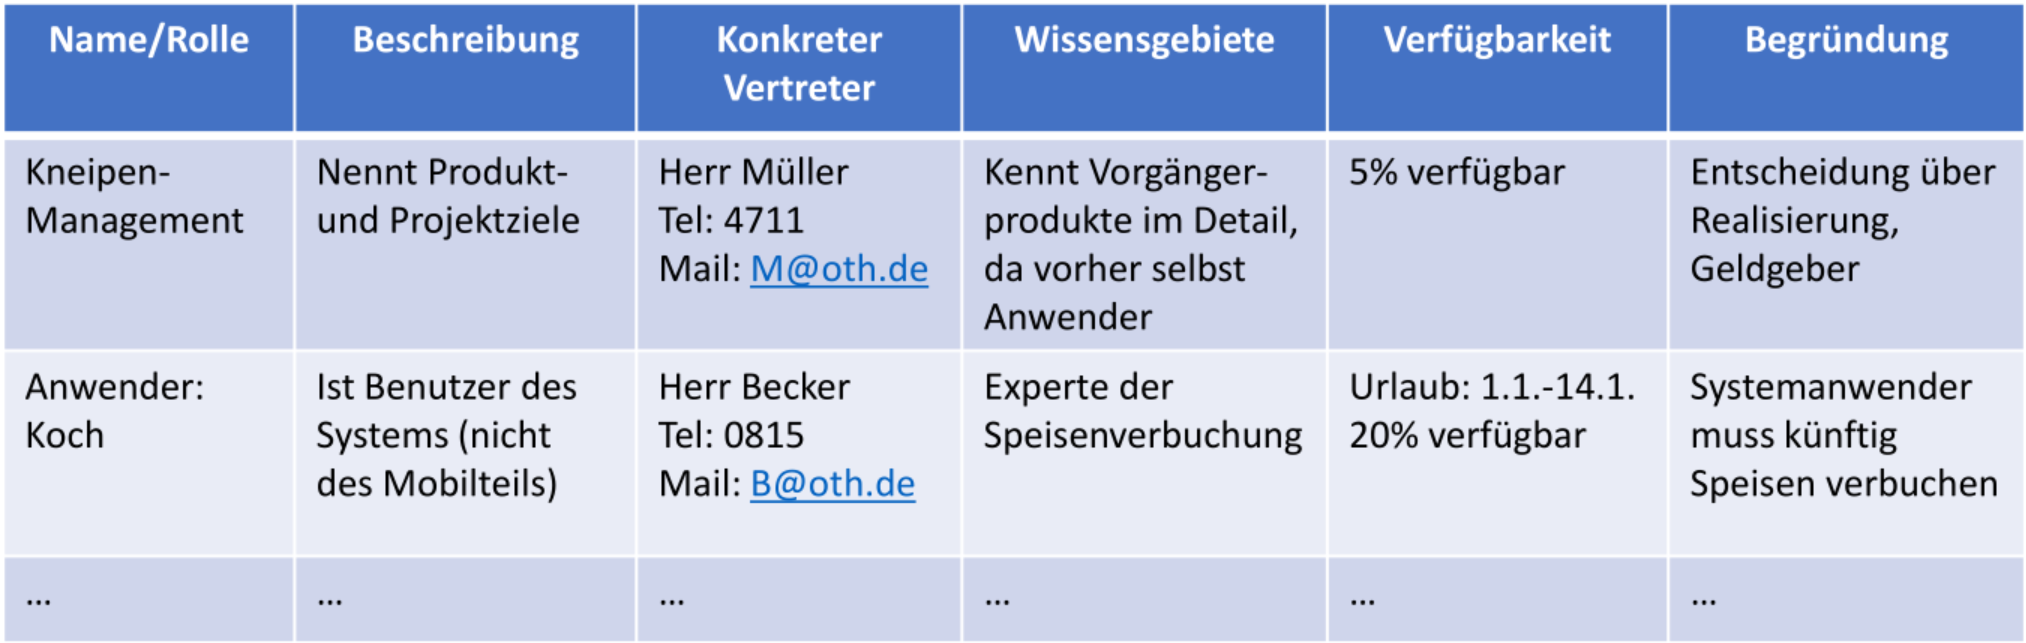
\includegraphics[width=1\textwidth]{Stakeholder-00}
    \caption{Stakeholderliste}
    \label{fig:Stakeholder-00}
\end{figure}

$ \rightarrow $ Übersehen von Stakeholdern kann zu unvollständigen Anforderungen führen

\subsubsection*{Checkliste zum Finden von Stakeholdern}

\begin{itemize}
    \item Wartungs- und Servicepersonal
    \begin{itemize}
        \item Wartung und Service muss unkompliziert und zügig durchzuführen sein
        \item Wichtig bei hohen Stückzahlen
    \end{itemize}
    \item Produktbeseitiger
    \begin{itemize}
        \item Wichtig, wenn ausgeliefertes Produkt nicht nur Software umfasst, Frage der Beseitigung (z.B. Umweltschutz), kann enormen Einfluss auf Zielsetzung von Produktentwicklung haben
    \end{itemize}
    \item Schulungs- und Trainingspersonal
    \begin{itemize}
        \item Liefern konkrete Anforderungen zu Bedienbarkeit, Vermittelbarkeit, Hilfesystem, Dokumentation, Erlernbarkeit
    \end{itemize}
    \item Marketing und Vertriebsabteilung
    \begin{itemize}
        \item Als interne Repräsentanten externer Kundenwünsche und Marktentwicklung
    \end{itemize}
    \item Systemschützer
    \begin{itemize}
        \item Stellen Anforderungen zum Schutz vor Fehlverhalten von Stakeholdern
    \end{itemize}
    \item Standards und Gesetze
    \begin{itemize}
        \item Vorhandene und zukünftige Standards/Gesetze berücksichtigen
    \end{itemize}
    \item Projekt- und Produktgegner
    \begin{itemize}
        \item Vor allem zu Beginn des Projekts möglichst mit einbeziehen, sonst drohen Konflikte
    \end{itemize}
    \item Kulturkreis
    \begin{itemize}
        \item Setzt Rahmenbedingungen, z.B. verwendete Symbolik, Begriffe, …
    \end{itemize}
    \item Meinungsführer und die öffentliche Meinung
    \begin{itemize}
        \item Beeinflussen oder schreiben Ziele vor, Zielmärkte berücksichtigen
    \end{itemize}
\end{itemize}


\subsection{Ermittlungstechniken}

\subsubsection*{Befragungstechniken}
\begin{itemize}
    \item \textbf{Interviews}: Direktes Gespräch zwischen Requirements Engineer und Stakeholder.
    \item \textbf{Fragebögen}: Standardisierte Fragen zur Sammlung von Anforderungen.
\end{itemize}

\subsubsection*{Dokumentengetrieben}
\begin{itemize}
    \item \textbf{Systemarchäologie}: Analyse der Dokumentation bestehender Systeme.
    \item \textbf{Perspektivenbasiertes Lesen}: Untersuchen von Dokumenten aus verschiedenen Perspektiven.
    \item \textbf{Wiederverwendung}: Bereits erstellte Anforderungen nutzen.
\end{itemize}

\subsubsection*{Beobachtungstechniken}
\begin{itemize}
    \item \textbf{Feldbeobachtung}: Beobachtung des Stakeholders in dessen gewohnter Umgebung.
    \item \textbf{Apprenticing}: Requirements Engineer erlernt die Tätigkeit des Stakeholders.
\end{itemize}

\subsubsection*{Kreativitätstechniken}
\begin{itemize}
    \item \textbf{Brainstorming}: Ideenfindung in Gruppen.
    \item \textbf{Perspektivenwechsel}: Betrachtung des Problems aus verschiedenen Blickwinkeln.
\end{itemize}


\subsection{Anforderungen dokumentieren}

\subsubsection*{Benutzeranforderungen (Was? und Wofür?):}
\begin{itemize}
    \item Aussagen in natürlicher Sprache (Vorteile/Nachteile?)
    \item Einfache Diagramme (Vorteile/Nachteile?)
    \item Beschreiben Dienste, die System leisten soll
    \item Beschreiben Randbedingungen unter denen System betrieben wird
    \item Systembeschreibung aus Kundensicht \textbf{(→ Lastenheft)}
\end{itemize}

\subsubsection*{Systemanforderungen (Wie? und Womit?):}
\begin{itemize}
    \item Detaillierte Festlegung von Funktionen, Diensten und Beschränkungen
    \item Beschreibung, was implementiert werden soll
    \item Systembeschreibung aus technischer Sicht \textbf{(→ Pflichtenheft))}
\end{itemize}

\subsubsection{Lastenheft}
\begin{itemize}
    \item Wird von Auftraggeber erstellt
    \item Beschreibung des \textbf{“Was”} und \textbf{"Wofür”}
    \item “Grobes” Pflichtenheft
    \item Details werden bewusst offen gelassen
\end{itemize}

\subsubsection{Pflichtenheft}
\begin{itemize}
    \item Wird vom Auftragnehmer erstellt
    \item Beschreibung des \textbf{Wie} und \textbf{“Womit”}
    \item Zu lieferndes System wird detailliert
    \item Systembeschreibung aus technischer Sicht
\end{itemize}


\subsubsection*{Templates nach Balzert:}

\noindent
\begin{minipage}[t]{0.45\textwidth}
    \textbf{Lastenheft}
    \begin{enumerate}
        \item Vision und Ziele
        \item Rahmenbedingungen
        \item Kontext und Überblick
        \item Funktionale Anforderungen
        \item Qualitätsanforderungen
    \end{enumerate}
\end{minipage}
\hfill
\begin{minipage}[t]{0.45\textwidth}
    \textbf{Pflichtenheft}
    \begin{enumerate}
        \item Vision und Ziele
        \item Rahmenbedingungen
        \item Kontext und Überblick
        \item Funktionale Anforderungen
        \item Qualitätsanforderungen
        \item Abnahmekriterien
        \item Subsystemstruktur (optional)
        \item Glossar
    \end{enumerate}
\end{minipage}

\vspace{2em}

\textit{→ das Pflichtenheft ist eine Verfeinerung des Lastenheftes}






\subsection{Anforderungen prüfen und abstimmen}

\subsubsection*{Prüfung}
\begin{itemize}
    \item \textbf{Inspektionen}: Systematische Überprüfung der Anforderungen.
    \item \textbf{Reviews}: Überprüfung durch Stakeholder und Fachexperten.
    \item \textbf{Walkthroughs}: Schritt-für-Schritt-Durchgang der Anforderungen.
\end{itemize}

\subsubsection*{Validierung}
\begin{itemize}
    \item Überprüfung jeder Anforderung gegen Visionen und Ziele.
    \item Stakeholder-Review und formale Abnahme.
\end{itemize}

\newpage


\subsection{Kano-Modell}

\begin{enumerate}
    \item Basis-Merkmale:
    \begin{itemize}
        \item Grundlegend, Kunden merken es bei Nichterfüllung (implizite Erwartungen)
        \item Nichterfüllung führt zu Unzufriedenheit, Erfüllung führt nicht zu Zufriedenheit
        \item Geringe Nutzensteigerung gegenüber Wettbewerbern
        \item Beispiel Auto: Sicherheit, Rostschutz
    \end{itemize}
    \item Leistungs-Merkmale:
    \begin{itemize}
        \item Kunden bewusst, beseitigen Unzufriedenheit oder schaffen Zufriedenheit
        \item Beispiel Auto: Fahreigenschaften, Beschleunigung, Lebensdauer, Verbrauch
    \end{itemize}
    \item Begeisterungs-Merkmale:
    \begin{itemize}
        \item Nutzen stiftend, unerwartet, zeichnen Produkt aus, rufen Begeisterung hervor
        \item Kleine Leistungssteigerung, hoher Nutzen
        \item Beispiel Auto: Sonderausstattung, besonderes Design, Hybridtechnologie
    \end{itemize}
    \item Unerhebliche Merkmale:
    \begin{itemize}
        \item Ohne Belang für Kunden, stiften keine Zufriedenheit, führen nicht zu Unzufriedenheit
        \item Beispiel Auto: Automatikgetriebe, Schiebedach (je nach Kundengruppe)
    \end{itemize}
    \item Rückweisungs-Merkmale:
    \begin{itemize}
        \item Führen bei Vorhandensein zu Unzufriedenheit, bei Fehlen keine Zufriedenheit
        \item Beispiel Auto: Rostflecken, abgelaufener TÜV
    \end{itemize}
\end{enumerate}

\vspace{2em}

\begin{figure}[h]
    \centering
    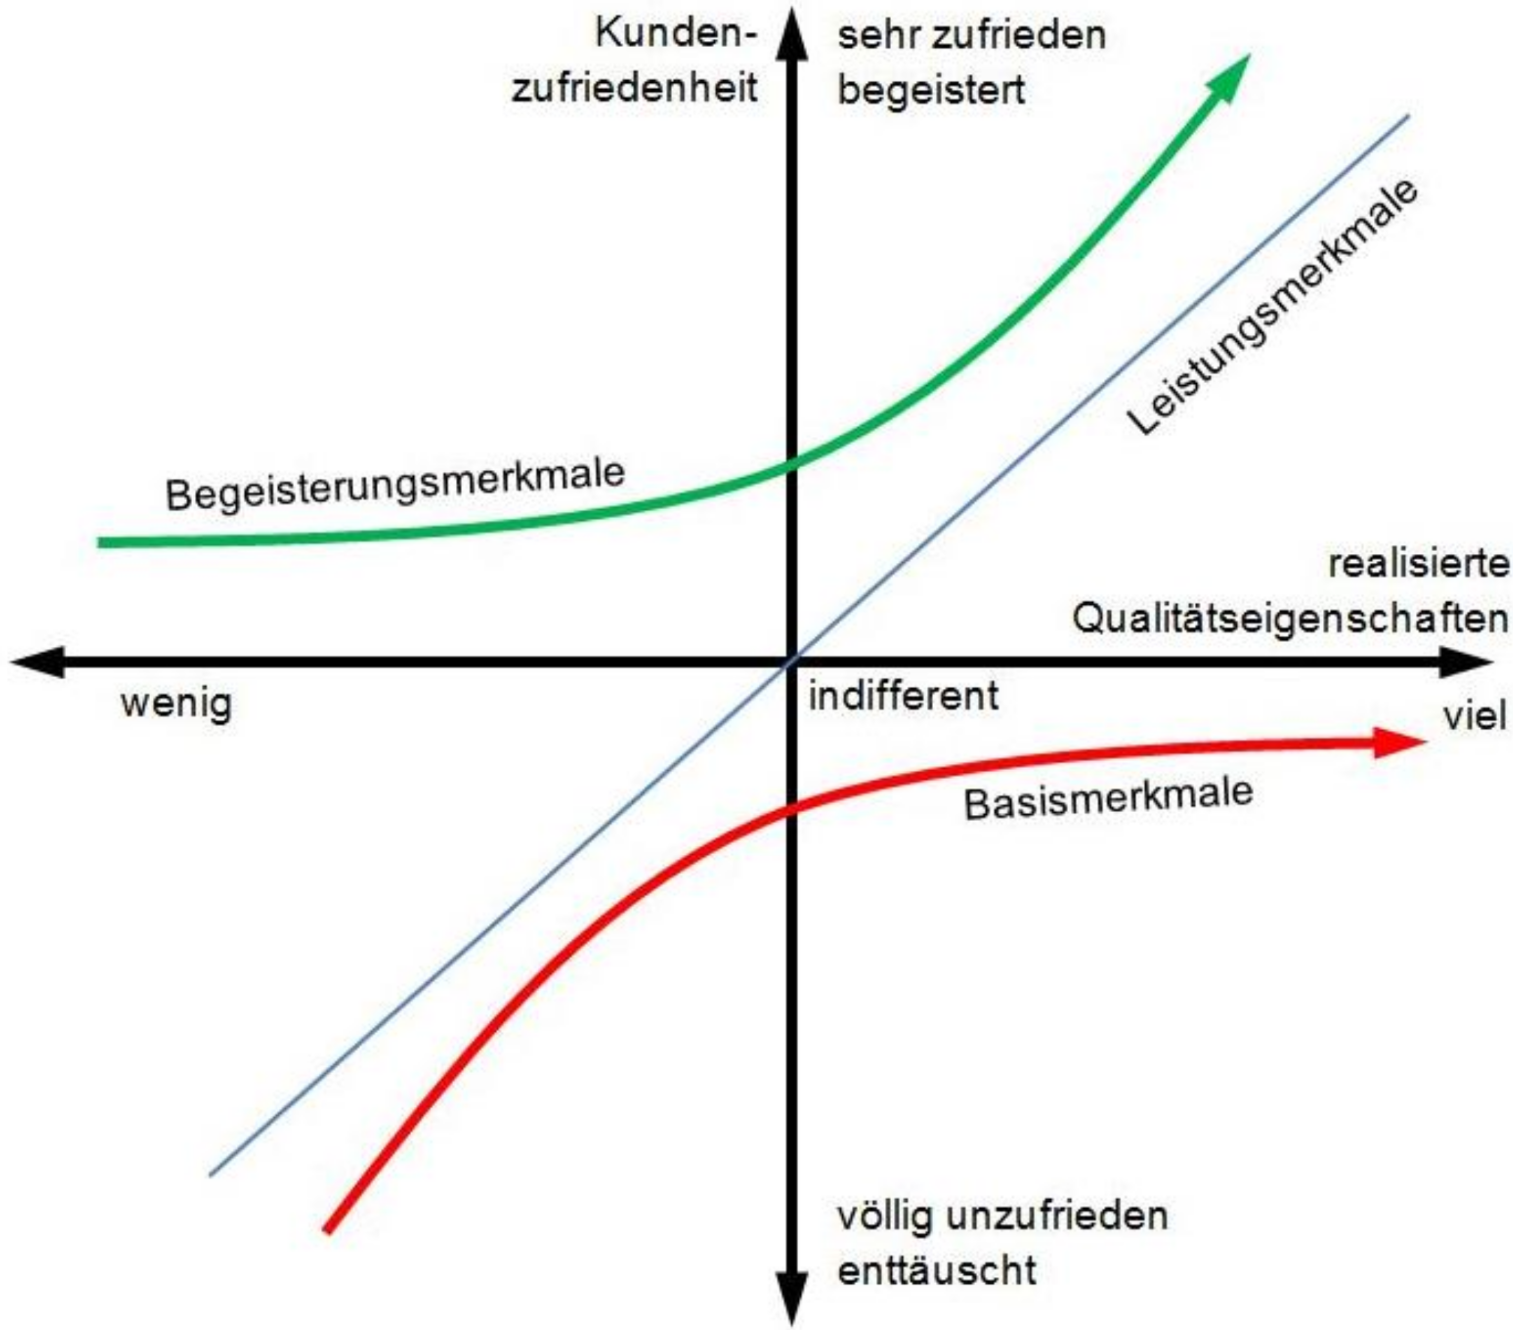
\includegraphics[width=0.5\textwidth]{Kano-00.png}
    \caption{Veranschaulichung des Kano-Modells}
    \label{fig:Kano-00}
\end{figure}

\newpage


Kano Modelle werden auf Basis von Kunden Befragungen ausgefüllt!

Hier ein Beispiel eines Kano Modells für intelligentes Krankenbett:

\vspace{1em}

\begin{figure}[h]
    \centering
    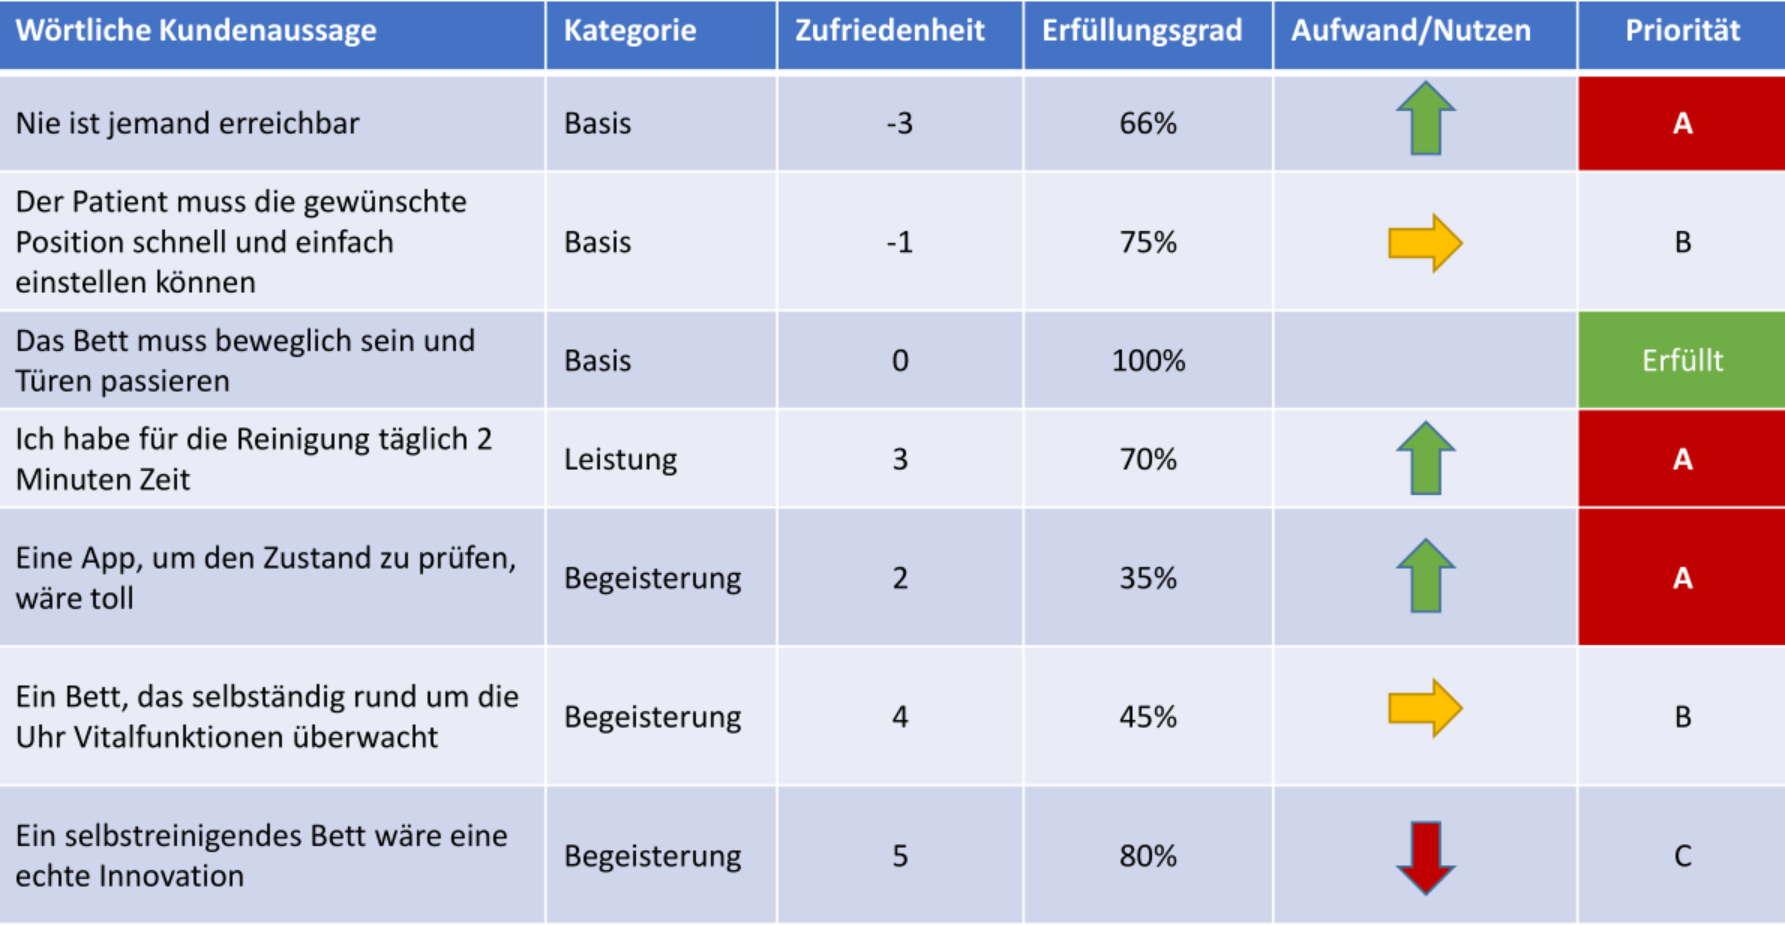
\includegraphics[width=0.8\textwidth]{Kano-01.png}
    \caption{Beispiel für Kano-Modell Tabelle}
    \label{fig:Kano-01}
\end{figure}


\begin{figure}[h]
    \centering
    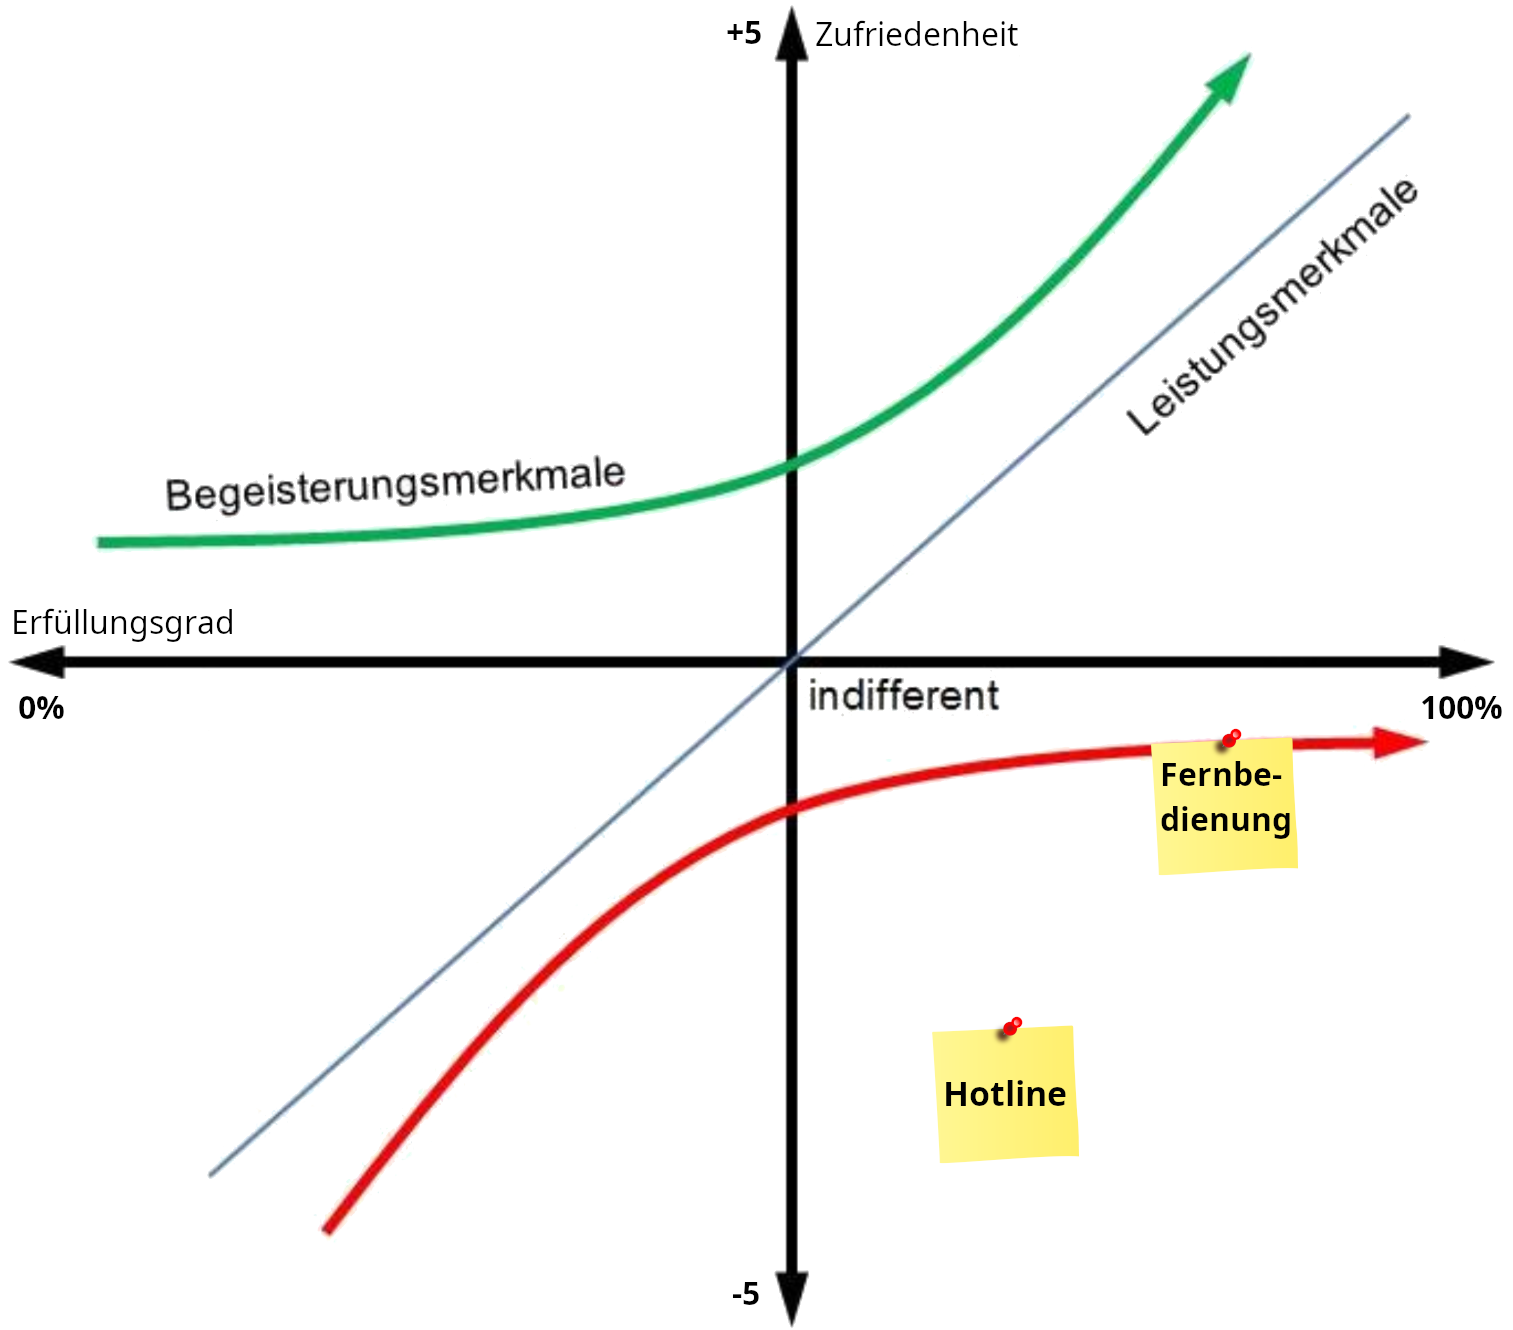
\includegraphics[width=0.5\textwidth]{Kano-02.png}
    \caption{Beispiel für Kano-Modell Graph}
    \label{fig:Kano-02}
\end{figure}

\vspace{2em}

\noindent \sloppy Die nicht erreichbare Hotline zum Beispiel, wird von den Kunden als -3 in der Zufriedenheit und 66\% im Erfüllungsgrad gewertet.
Auf dem Graphen ist dieses Merkmal unter der Basismerkmal Kurve und somit sehr schlecht.\\
Dadurch ist der Aufwand/Nutzen hoch und die Priorität 'A'.

\newpage



\subsection{Best practices}

\begin{itemize}
    \item Kunden und Benutzer einbinden
    \item Alle möglichen RE-Quellen identifizieren und konsultieren
    \item Erfahrene Projektmanager und Teammitglieder einsetzen
    \item 15 – 30 \% der Ressourcen für RE vorsehen
    \item Anforderungsschablonen und Beispiele zur Verfügung stellen
    \item Gute Beziehungen zu allen Beteiligten und Betroffenen herstellen
    \item Anforderungen priorisieren
    \item Ergänzende Modelle gemeinsam mit Prototypen entwickeln
    \item Eine Nachverfolgungsmatrix pflegen
    \item Peer Reviews durch Benutzer, Szenarien und Walk-Throughs zur Validierung und Verifizierung der Anforderungen durchführen
\end{itemize}



\subsection{Erfassung von Anforderungen}

\subsubsection{Requirements Analysis}

\begin{enumerate}
    \item Erfassung der Systemaufgaben mit \textbf{Use Cases}
    \item Beschreibung der Aufgaben mit \textbf{Aktivitätsdiagrammen}
    \item (optional) Formalisierung der Beschreibungen in \textbf{Anforderungen}
    \item Aufbau eines tieferen Verständnisses durch \textbf{Klassenmodellierung} und \textbf{Sequenzdiagramme} (Grobdesign)
\end{enumerate}

\vspace{1em}

$ \rightarrow $ \textbf{Was} sind die Hauptaufgaben des Systems?

$ \rightarrow $ \textbf{Wer} ist an den Aufgaben beteiligt?

$ \rightarrow $ \textbf{Welche Schritte} gehören zur Aufgabenerfüllung?

\newpage



\newpage


\section{Objektorientierte Analyse (OOA)} % --- Objektorientierte Analyse (OOA) ------------------------------------------------------------------------------------


\subsection{Kontext-Diagramme}

\textbf{Früh in Analysephase:} Systemkontext erfassen und dokumentieren

\begin{figure}[h]
    \centering
    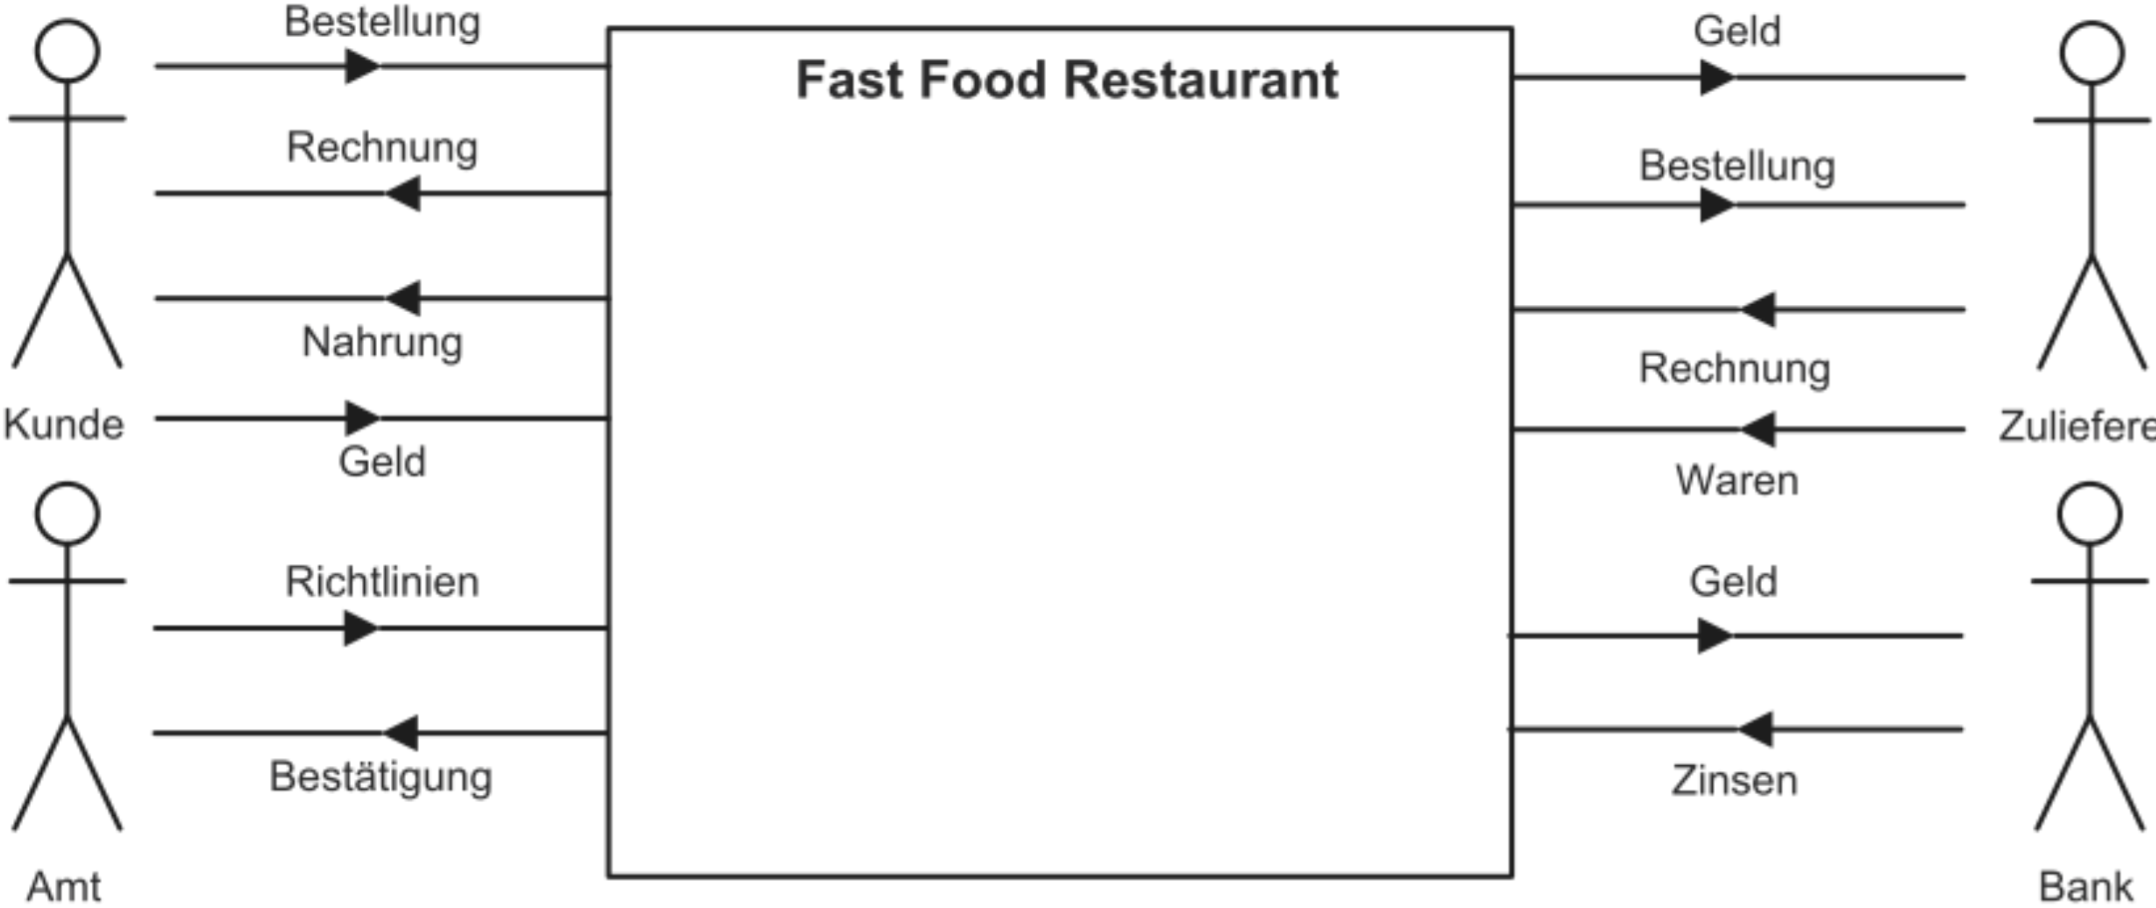
\includegraphics[width=0.75\textwidth]{KontextDiagramm-00.png}
    \caption{Beispiel eines Kontext Diagramm}
    \label{fig:KontextDiagramm-00}
\end{figure}

\vspace{5em}

\centering $ \downarrow $ \textbf{Das Folgende Kapitel 'UML und Diagrammtypen' ist Teil der OOA} $ \downarrow $


\raggedright \section{UML und Diagrammtypen}


\begin{figure}[h]
    \centering
    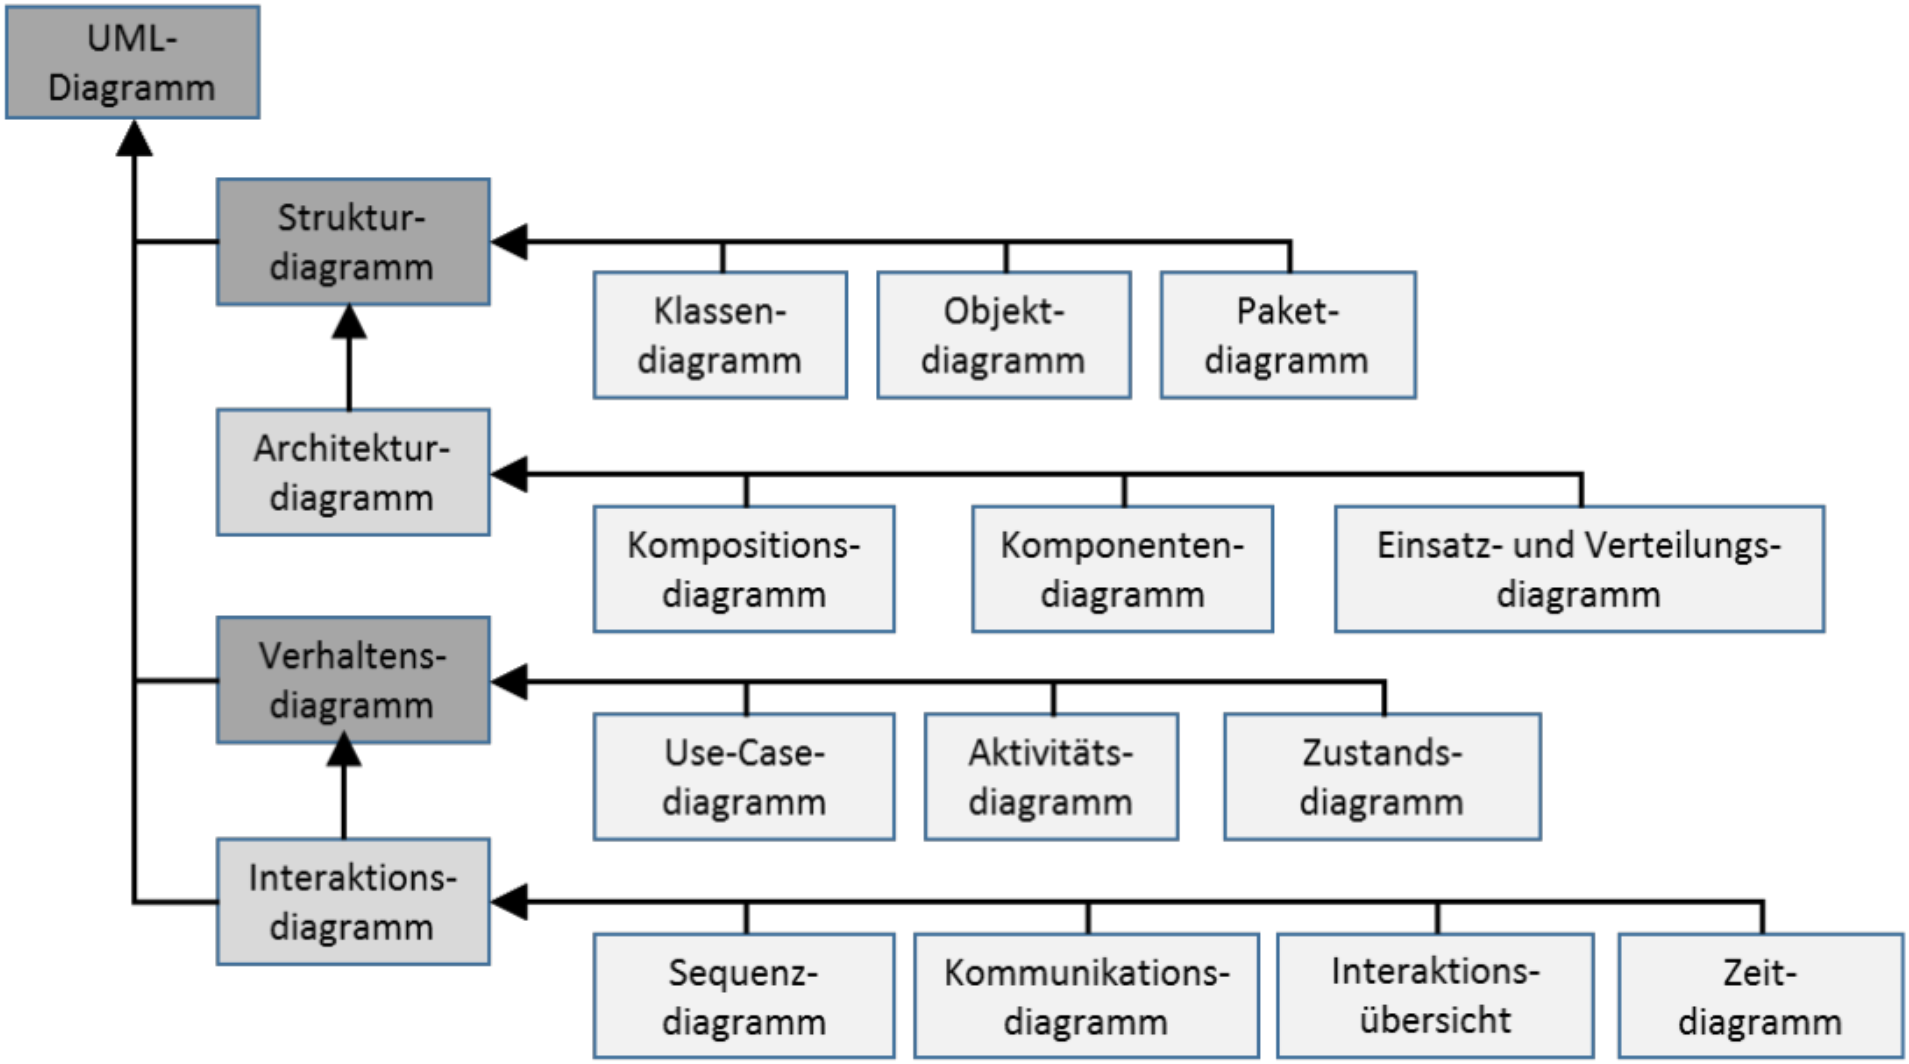
\includegraphics[width=0.75\textwidth]{UML-00.png}
    \caption{UML-Diagramme}
    \label{fig:UML-00}
\end{figure}


\newpage


\subsection{Use-Case Diagramme}


\noindent \textbf{Ziel und Definition:} Spezifiziert Sequenz von Aktionen einschließlich möglicher Varianten, die das System in Interaktion mit Akteuren auslöst. Es ist als Black-Box zu verstehen!

\vspace{1em}

\noindent\textbf{Erfragung des “WAS”?}
\begin{itemize}
    \item Was sind die Hauptaufgaben des Systems?
    \item Wer ist beteiligt?
    \item Welche Schritte gehören zur Aufgabenerfüllung?
    \item Aufgaben als Use Cases, Beteiligte als Akteure.
\end{itemize}

\vspace{1em}

\noindent\textbf{Struktur eines Use Cases:}
\begin{itemize}
    \item Titel, Kurzbeschreibung, Aktoren, Vorbedingungen, Ablauf, Auswirkungen, Anmerkungen.
\end{itemize}

\vspace{1em}

\noindent\textbf{Akteure:} Ein Akteur ist ein Objekt der Systemumgebung, das mit dem System interagiert und Use Cases auslösen kann. Akteure können Personen, externe Geräte oder Nachbarsysteme sein.

\vspace{3em}

\subsubsection{Standardelemente}

\begin{figure}[ht]
    \centering
    \begin{minipage}[t]{0.30\textwidth}
        \centering Aktor \\
        \vspace{1em}
        \centering 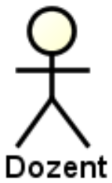
\includegraphics[width=0.2\textwidth]{UseCase-00.png}
    \end{minipage}
    \centering
    \begin{minipage}[t]{0.30\textwidth}
        \centering Use Case \\
        \vspace{1em}
        \centering 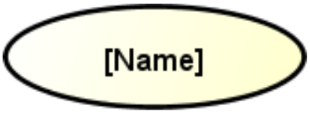
\includegraphics[width=0.5\textwidth]{UseCase-01.png}
    \end{minipage}
    \centering
    \begin{minipage}[t]{0.30\textwidth}
        \centering Systemgrenze \\
        \vspace{1em}
        \centering 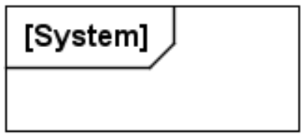
\includegraphics[width=0.5\textwidth]{UseCase-02.png}
    \end{minipage}
\end{figure}

\vspace{1em}

\begin{figure}[ht]
    \centering
    \begin{minipage}[t]{0.45\textwidth}
        \centering 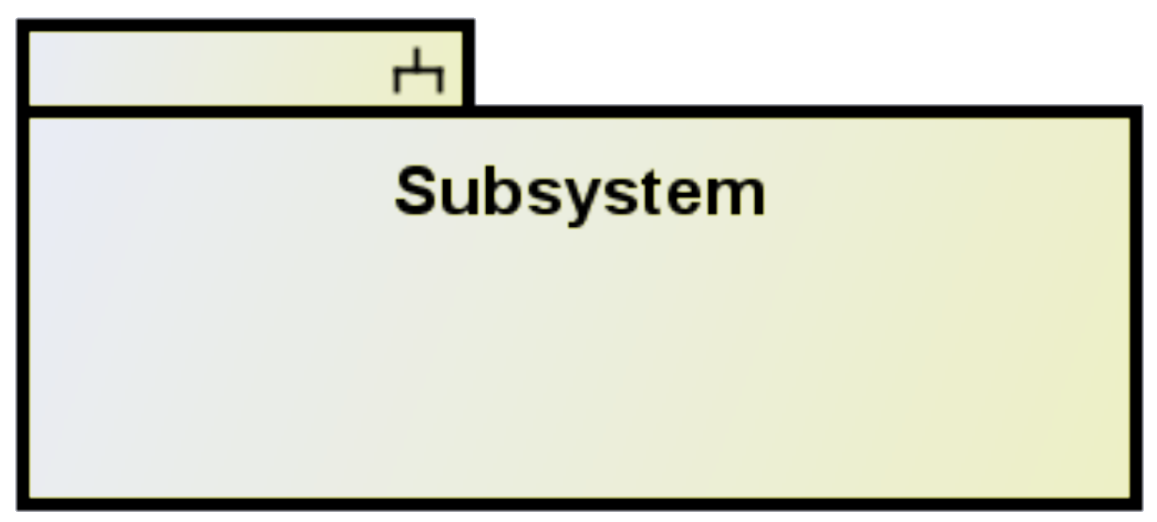
\includegraphics[width=0.4\textwidth]{UseCase-08.png} \\
        \vspace{1em}
        \centering Subsystem
    \end{minipage}
    \centering
    \begin{minipage}[t]{0.45\textwidth}
        \centering 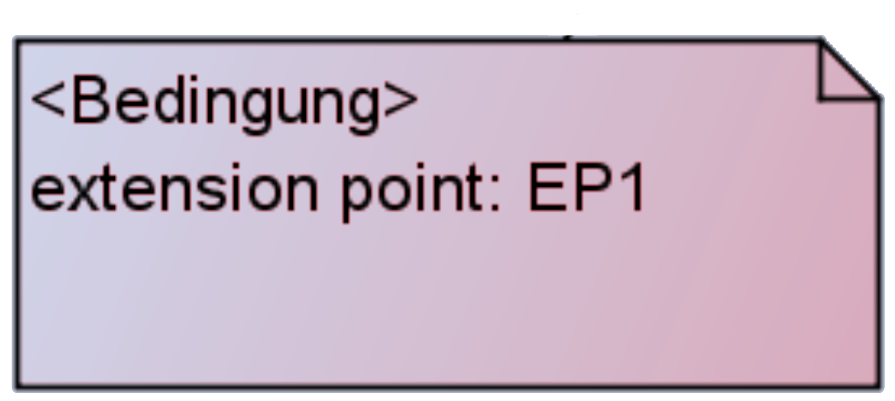
\includegraphics[width=0.4\textwidth]{UseCase-09.png} \\
        \vspace{1em}
        \centering Bedingung
    \end{minipage}
\end{figure}

\vspace{1em}

\begin{figure}[ht]
    \centering
    \begin{minipage}[t]{0.45\textwidth}
        \centering 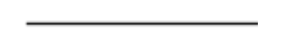
\includegraphics[width=0.4\textwidth]{UseCase-03.png} \\
        \vspace{1em}
        \centering Kommunikationsbeziehung zwischen Aktoren und Use Cases
    \end{minipage}
    \centering
    \begin{minipage}[t]{0.45\textwidth}
        \centering 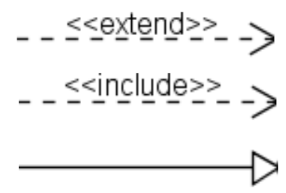
\includegraphics[width=0.4\textwidth]{UseCase-04.png} \\
        \vspace{1em}
        \centering Beziehung zwischen \\ Anwendungsfällen
    \end{minipage}
\end{figure}





\newpage

\subsubsection*{Beispiele}
\vspace{1em}

\centering Vollständiges Use-Case-Diagramm \\
\begin{figure}[h]
    \centering
    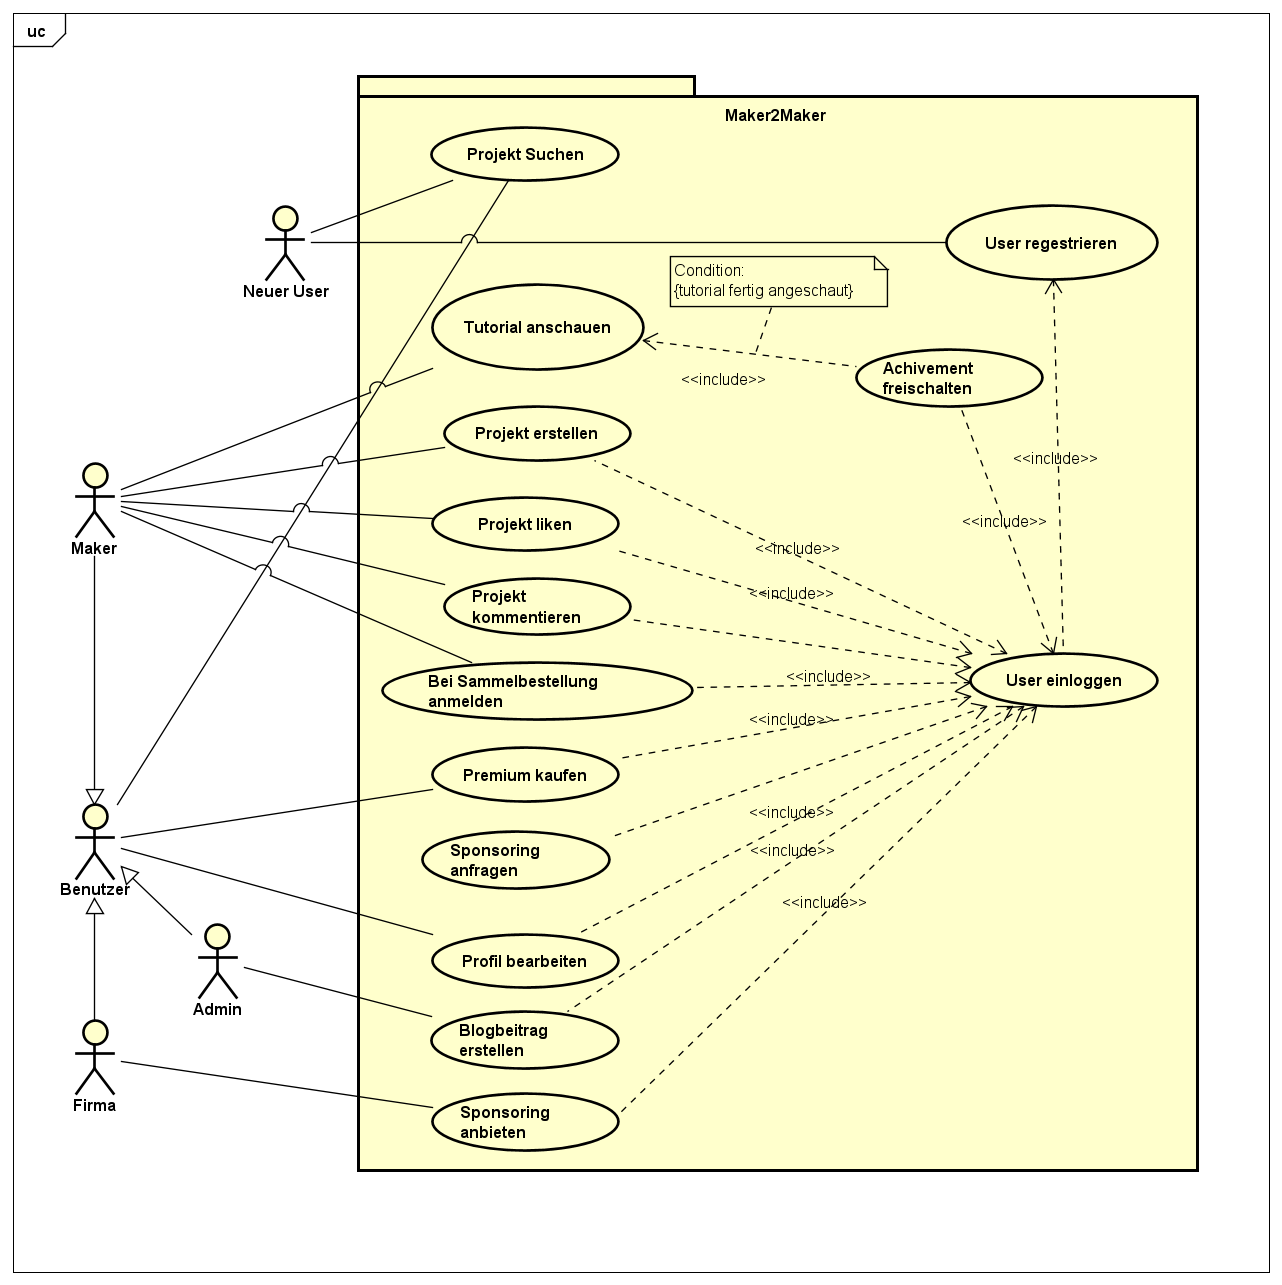
\includegraphics[width=0.70\textwidth]{UseCase-07.png}
    \label{fig:UseCase-07}
\end{figure}

\vspace{1em}

\centering Use-Case-Diagramm mit Subsystem \\
\begin{figure}[h]
    \centering
    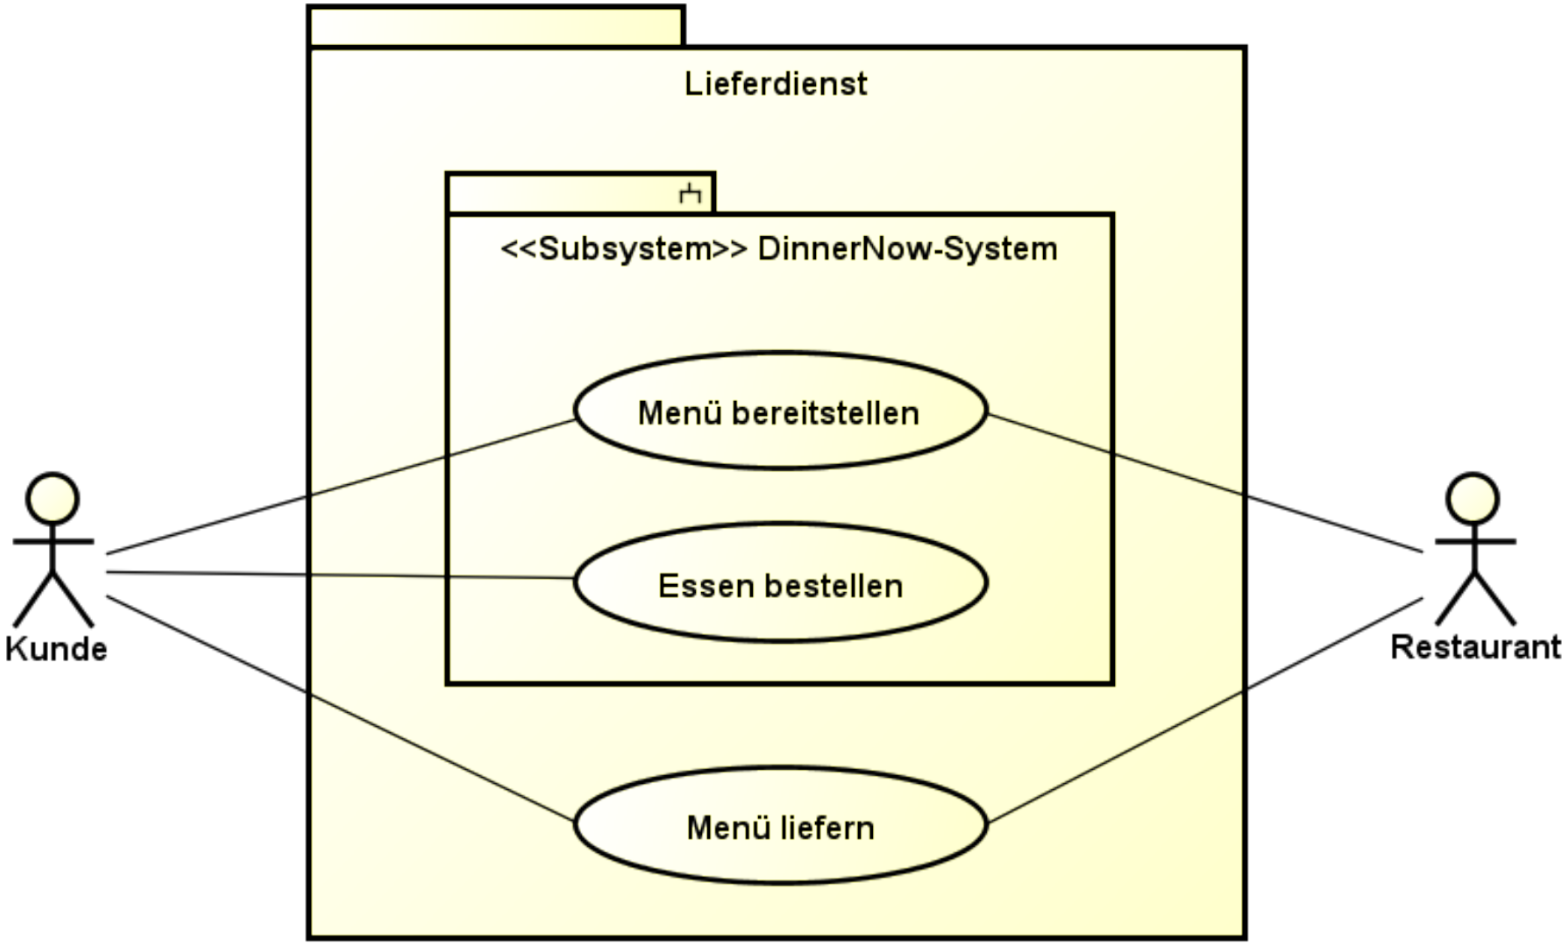
\includegraphics[width=0.5\textwidth]{UseCase-10.png}
    \label{fig:UseCase-10}
\end{figure}

\newpage



\raggedright \subsubsection{<<include>>}

\begin{itemize}
    \item Visualisiert, dass Use Case A das Verhalten von Use Case B importiert
\end{itemize}

\begin{figure}[h]
    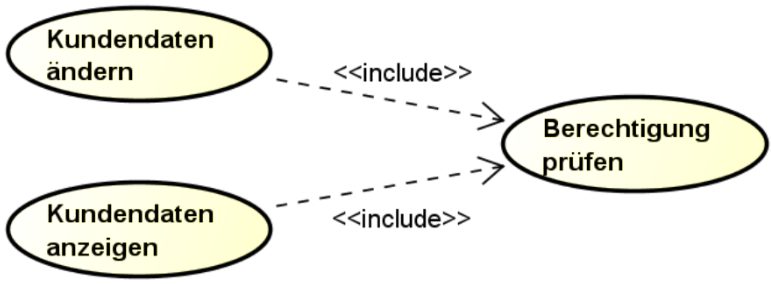
\includegraphics[width=0.3\textwidth]{UseCase-11.png}
    \label{fig:UseCase-11}
\end{figure}

\raggedright \subsubsection{<<extend>>}

\begin{itemize}
    \item Verhalten von Use-Case 2 kann durch Use-Case 1 erweitert werden (muss aber nicht)
    \item Ein Use Case darf mehrere Erweiterungspunkte besitzen
\end{itemize}

\begin{figure}[h]
    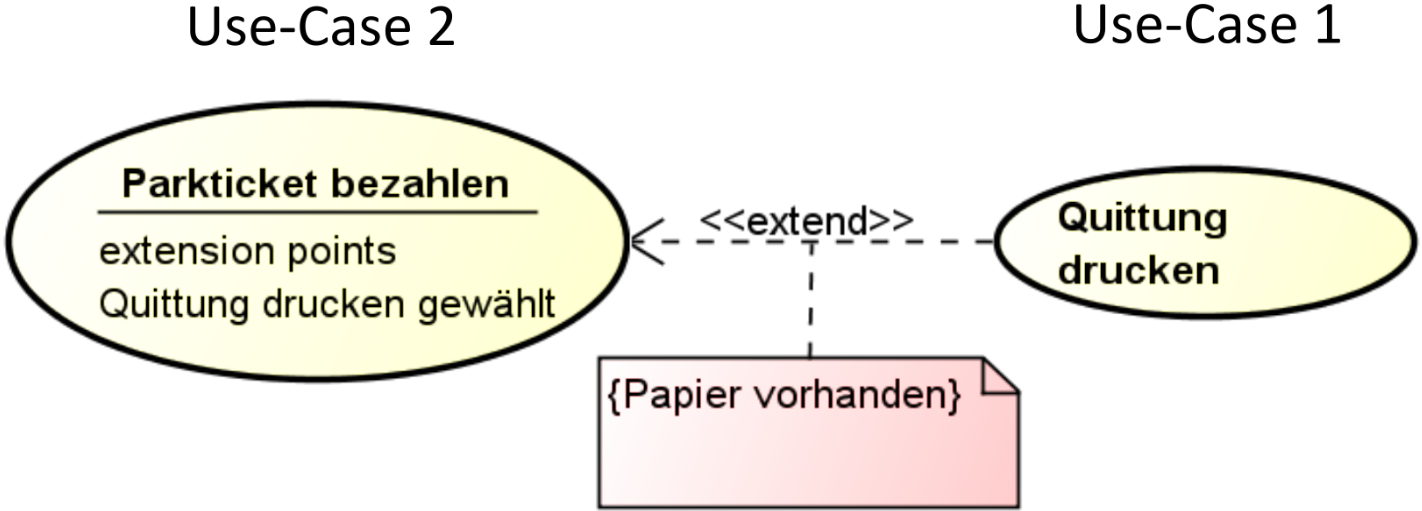
\includegraphics[width=0.3\textwidth]{UseCase-12.png}
    \label{fig:UseCase-12}
\end{figure}

\textbf{Achtung:} Pfeil weist in die Richtung des Use-Cases, der erweitert werden soll


\subsubsection{Use-Case Definitionen}

\subsubsection*{Beispiele}

\begin{figure}[ht]
    \centering
    \begin{minipage}[t]{0.45\textwidth}
        \centering 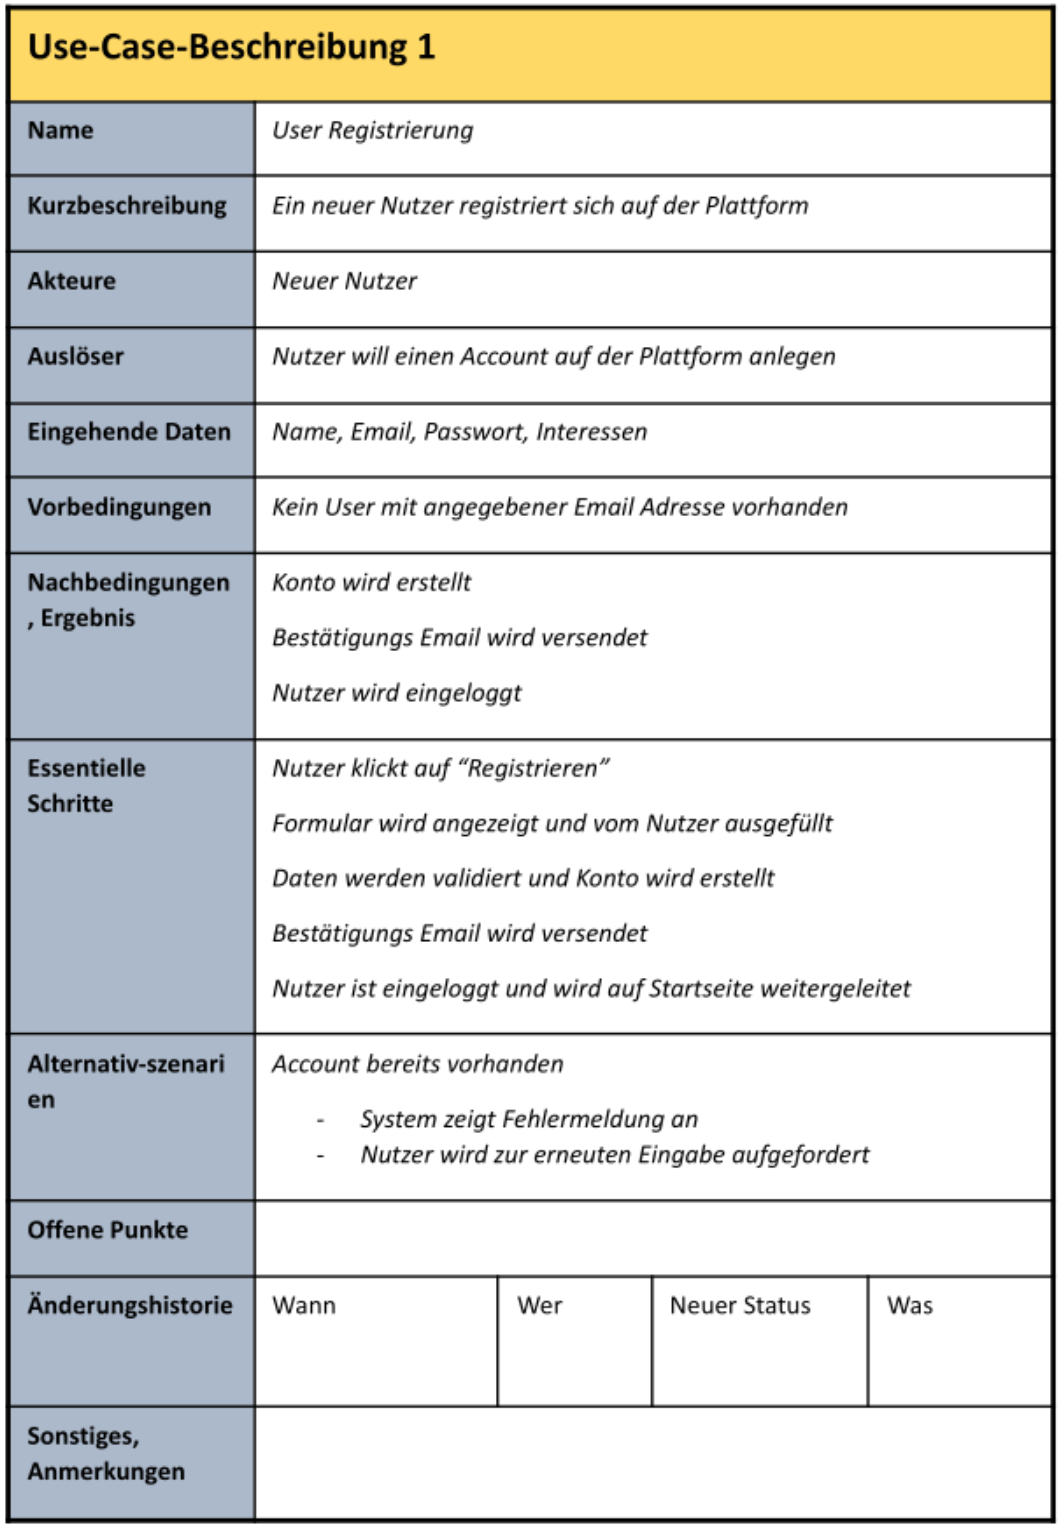
\includegraphics[width=0.9\textwidth]{UseCase-13.png} \\
    \end{minipage}
    \centering
    \begin{minipage}[t]{0.45\textwidth}
        \centering 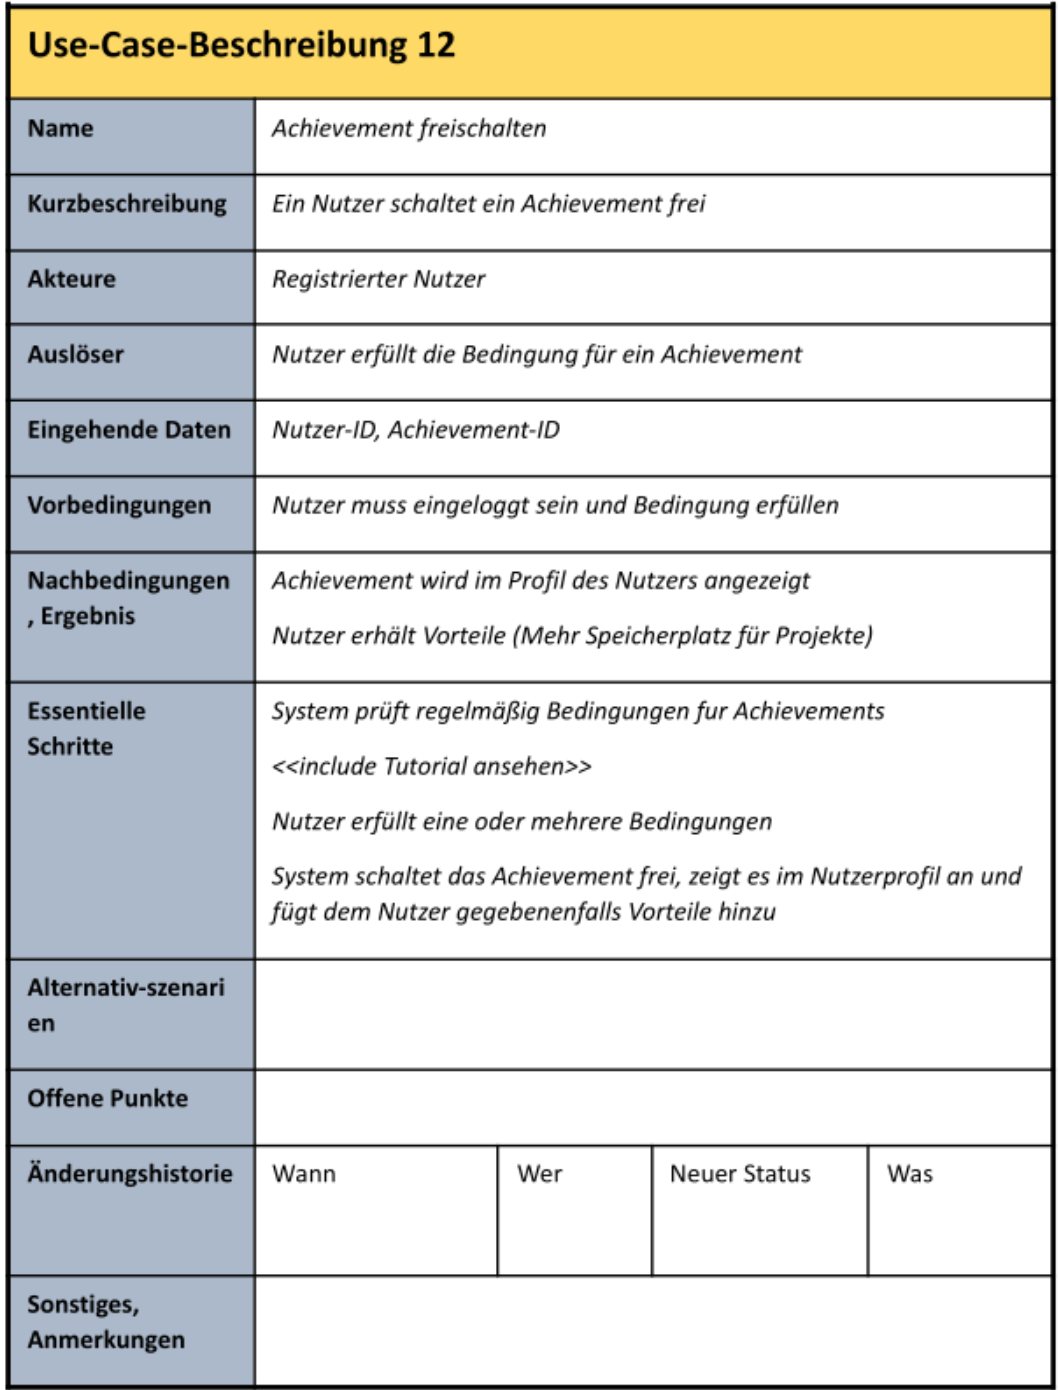
\includegraphics[width=0.9\textwidth]{UseCase-14.png} \\
        \vspace{1em}
        \centering mit <<include>>
    \end{minipage}
\end{figure}



\subsection{Aktivitätsdiagramme}

\vspace{2em}

\centering
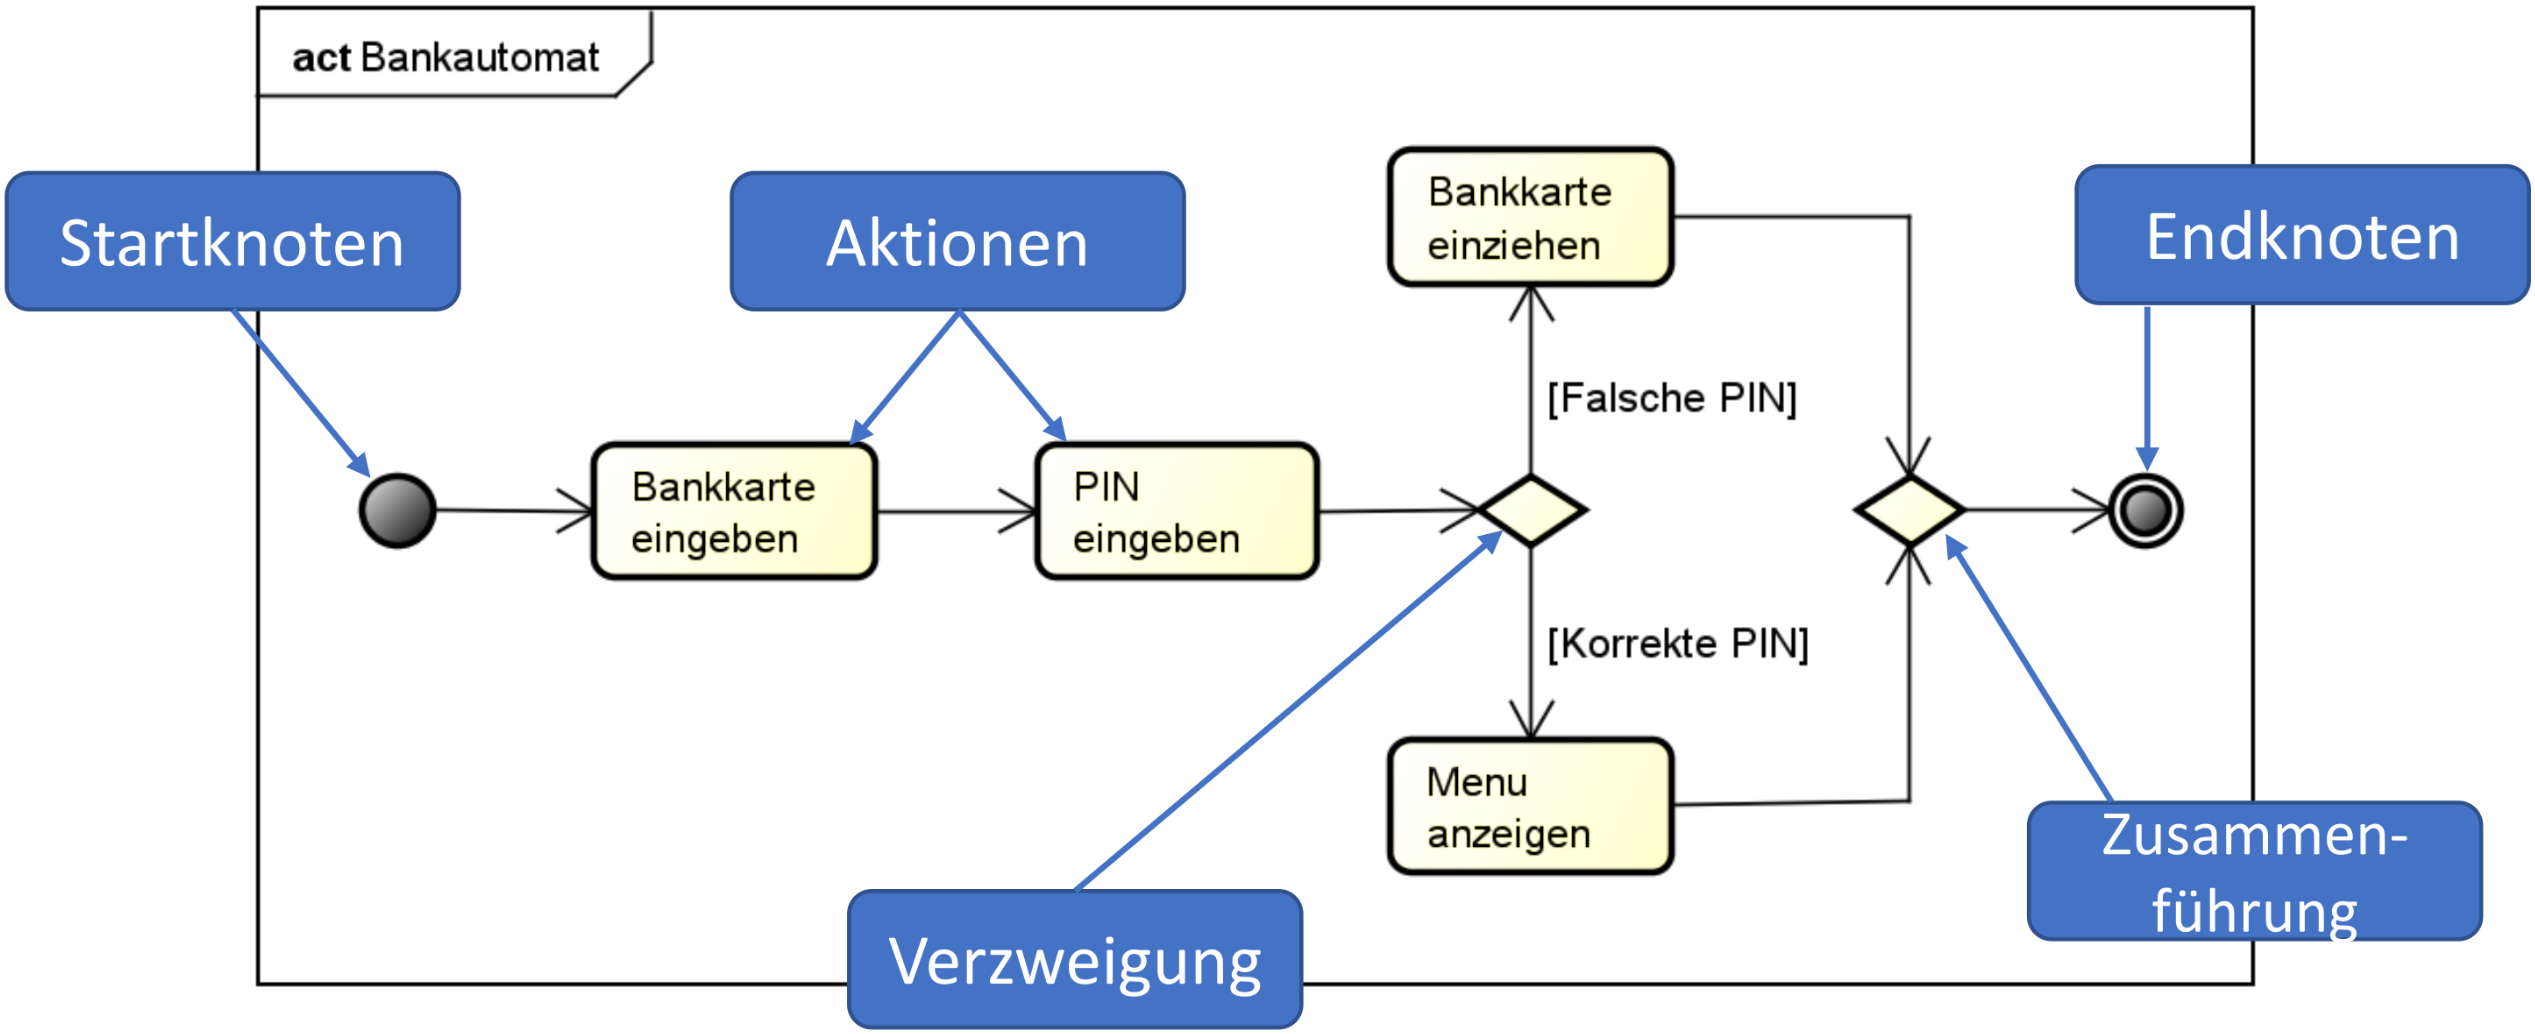
\includegraphics[width=0.5\textwidth]{Aktivitaet-00.png}


\raggedright Jede Aktivität hat nur \textbf{eine} eingehende Kante und \textbf{eine} ausgehende Kante!

\vspace{2em}

\raggedright \subsubsection{Verzweigung und Zusammenführung}

\centering
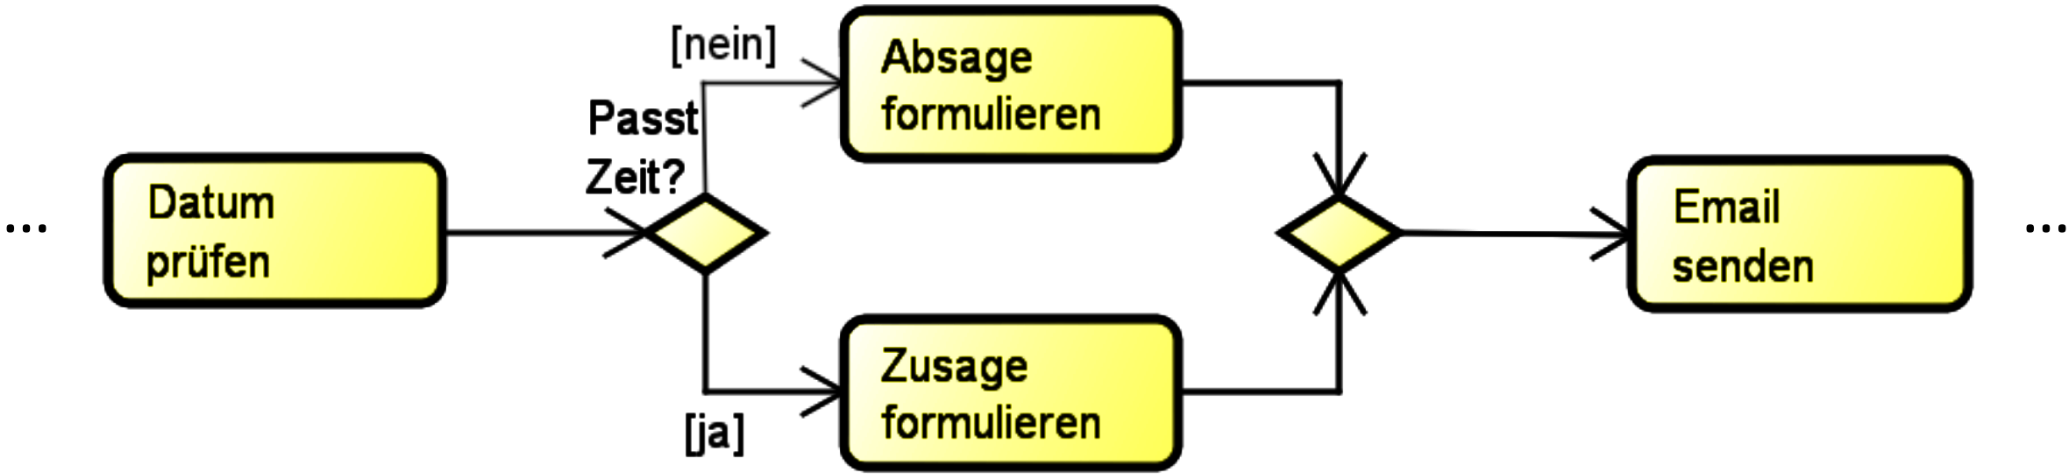
\includegraphics[width=0.75\textwidth]{Aktivitaet-03.png}

\vspace{2em}

\raggedright \subsubsection{Fork und Join}

\centering
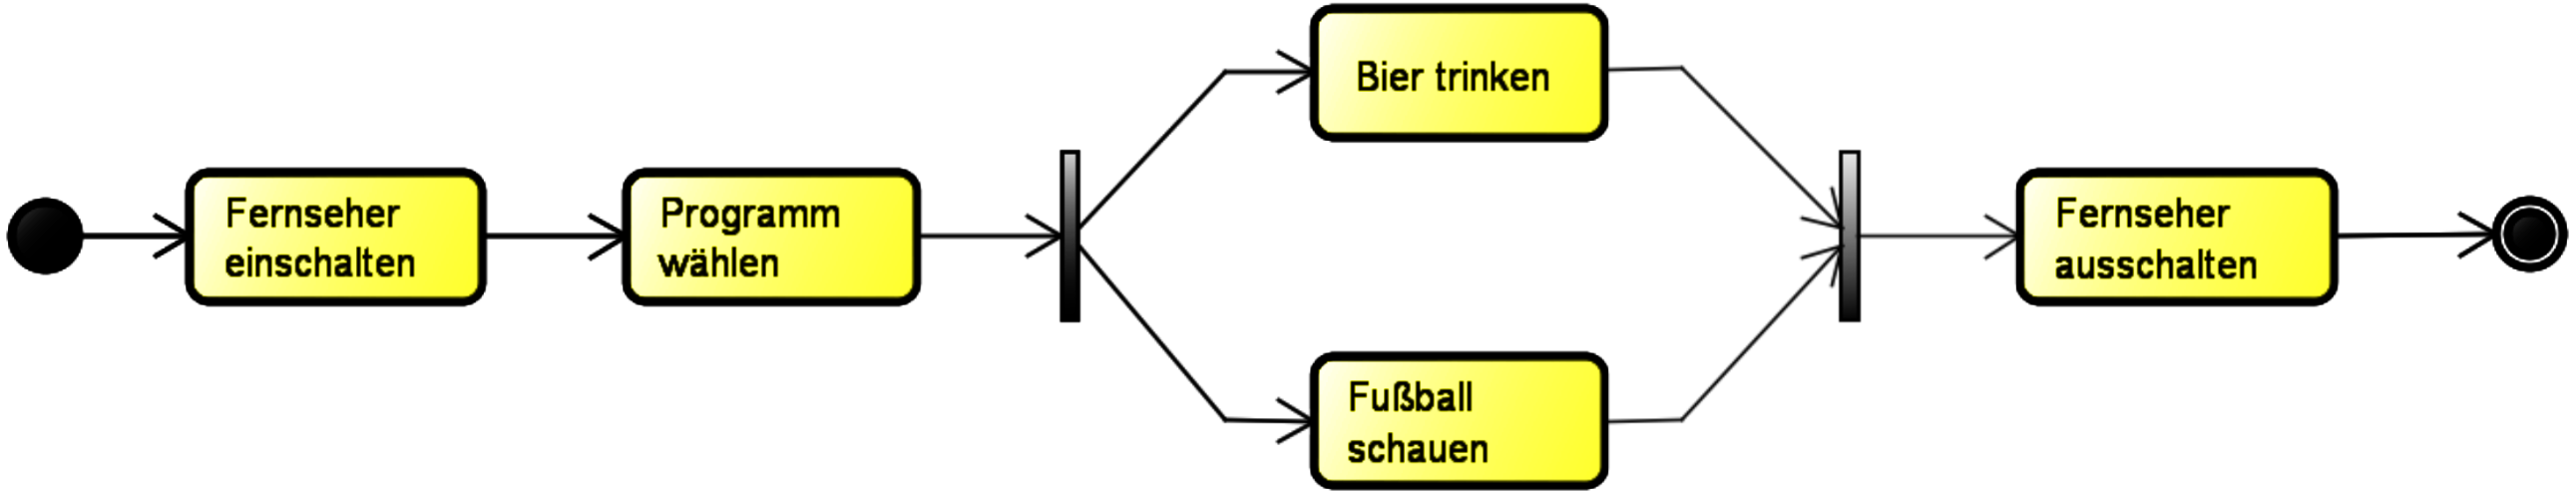
\includegraphics[width=0.75\textwidth]{Aktivitaet-02.png}

\vspace{2em}

\raggedright \subsubsection{Übersicht aller Elemente}

\centering
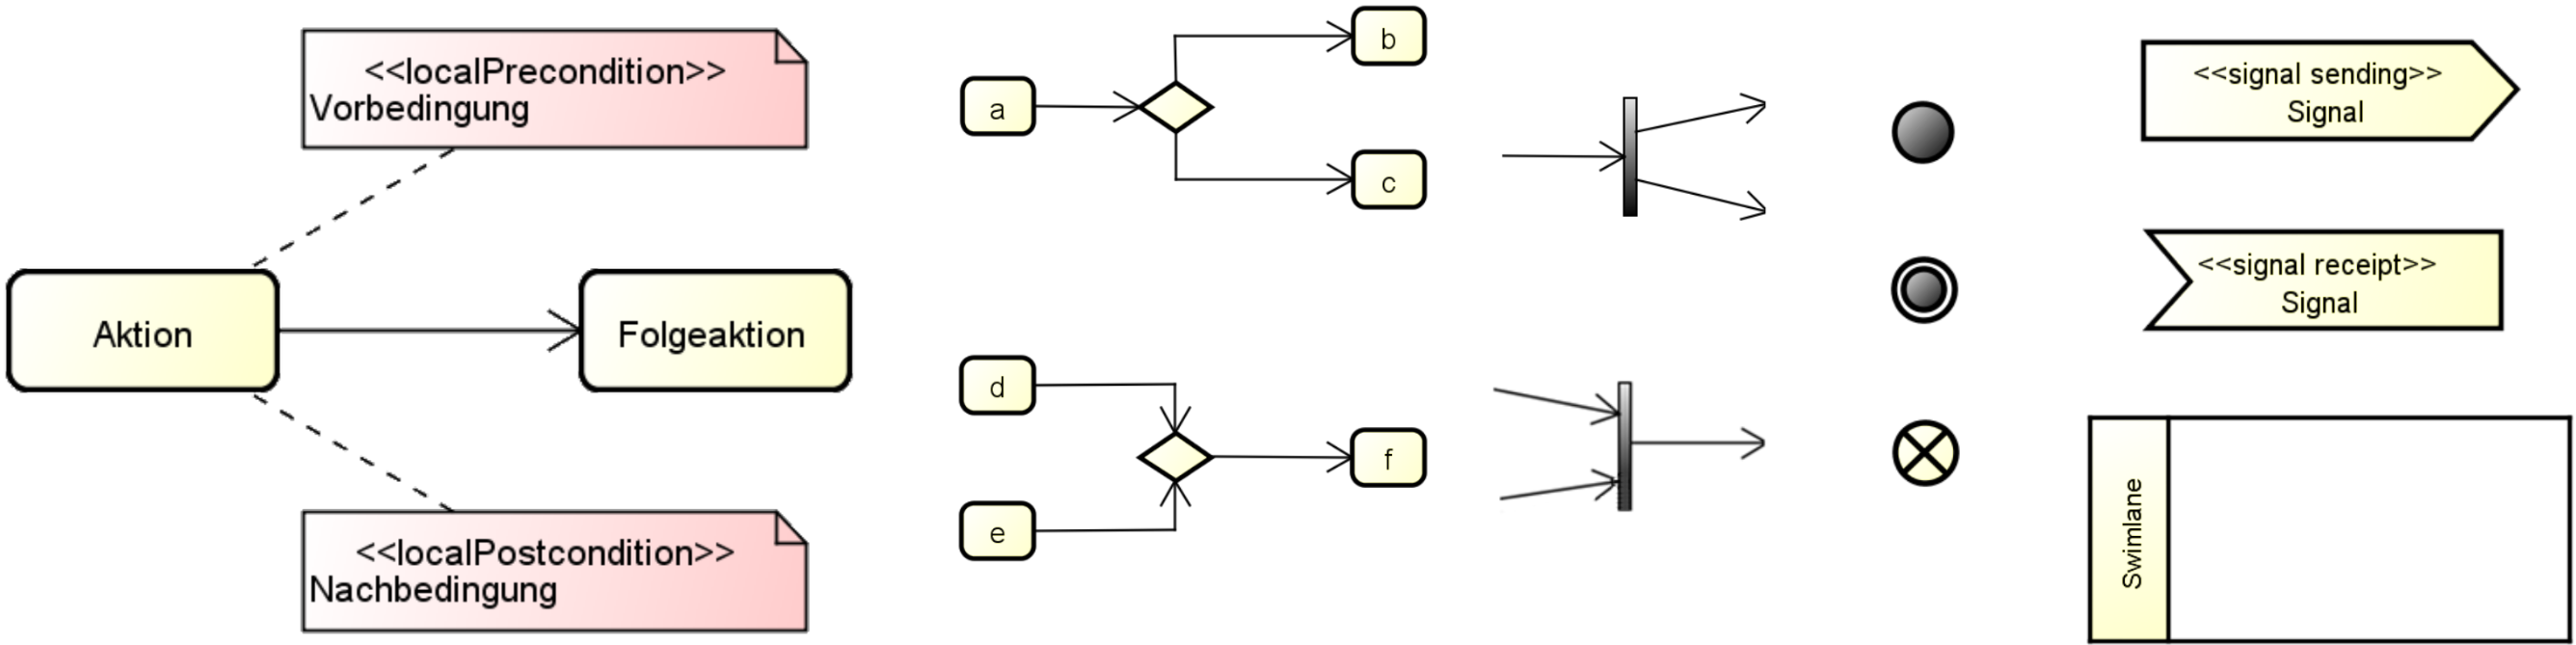
\includegraphics[width=0.75\textwidth]{Aktivitaet-01.png}

\newpage

\centering
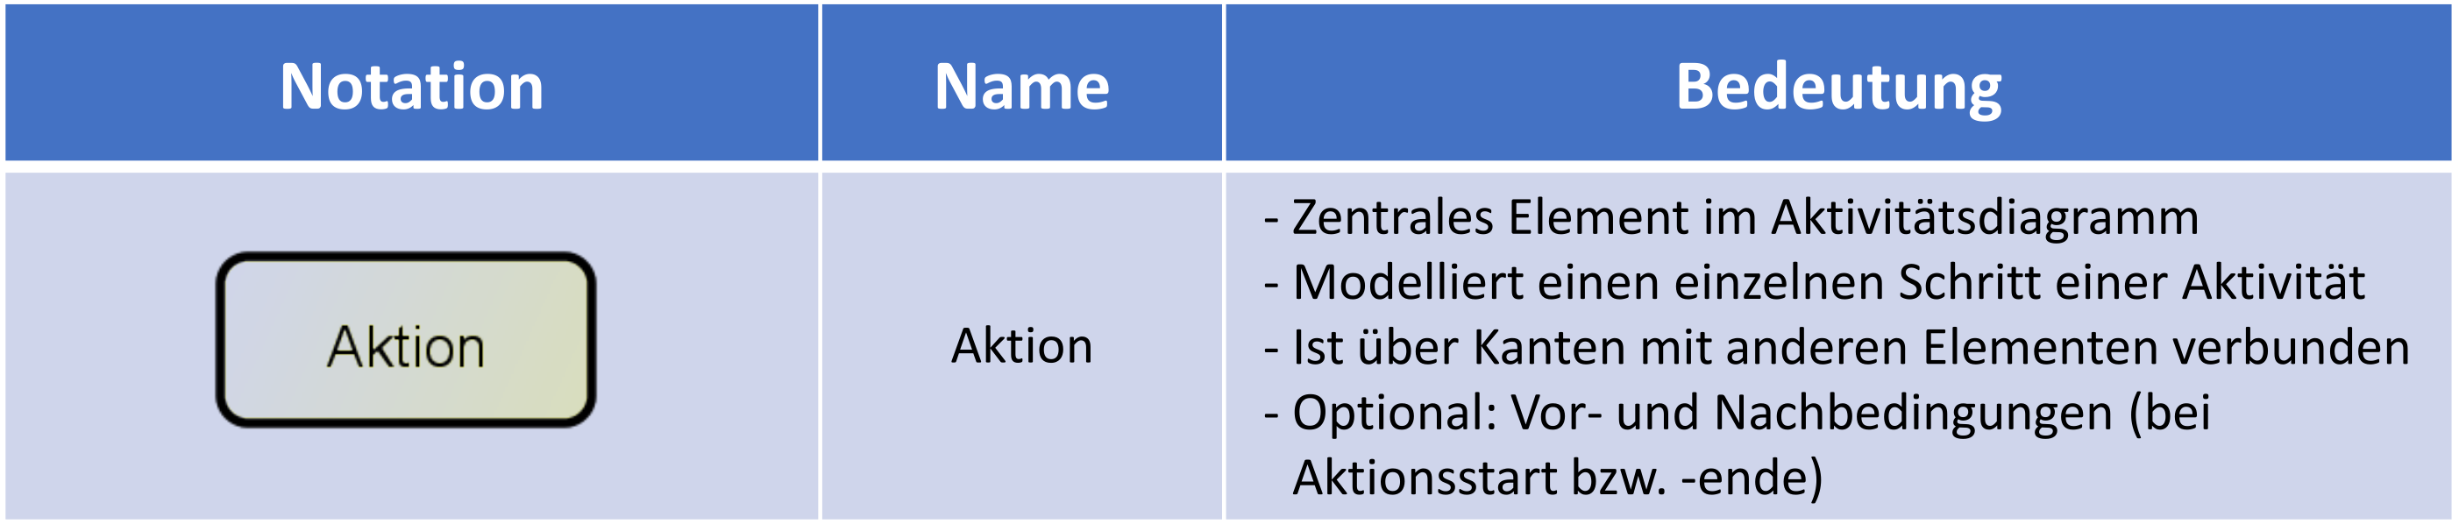
\includegraphics[width=0.75\textwidth]{Aktivitaet-Tabellen/1.png}

\vspace{1em}

\centering
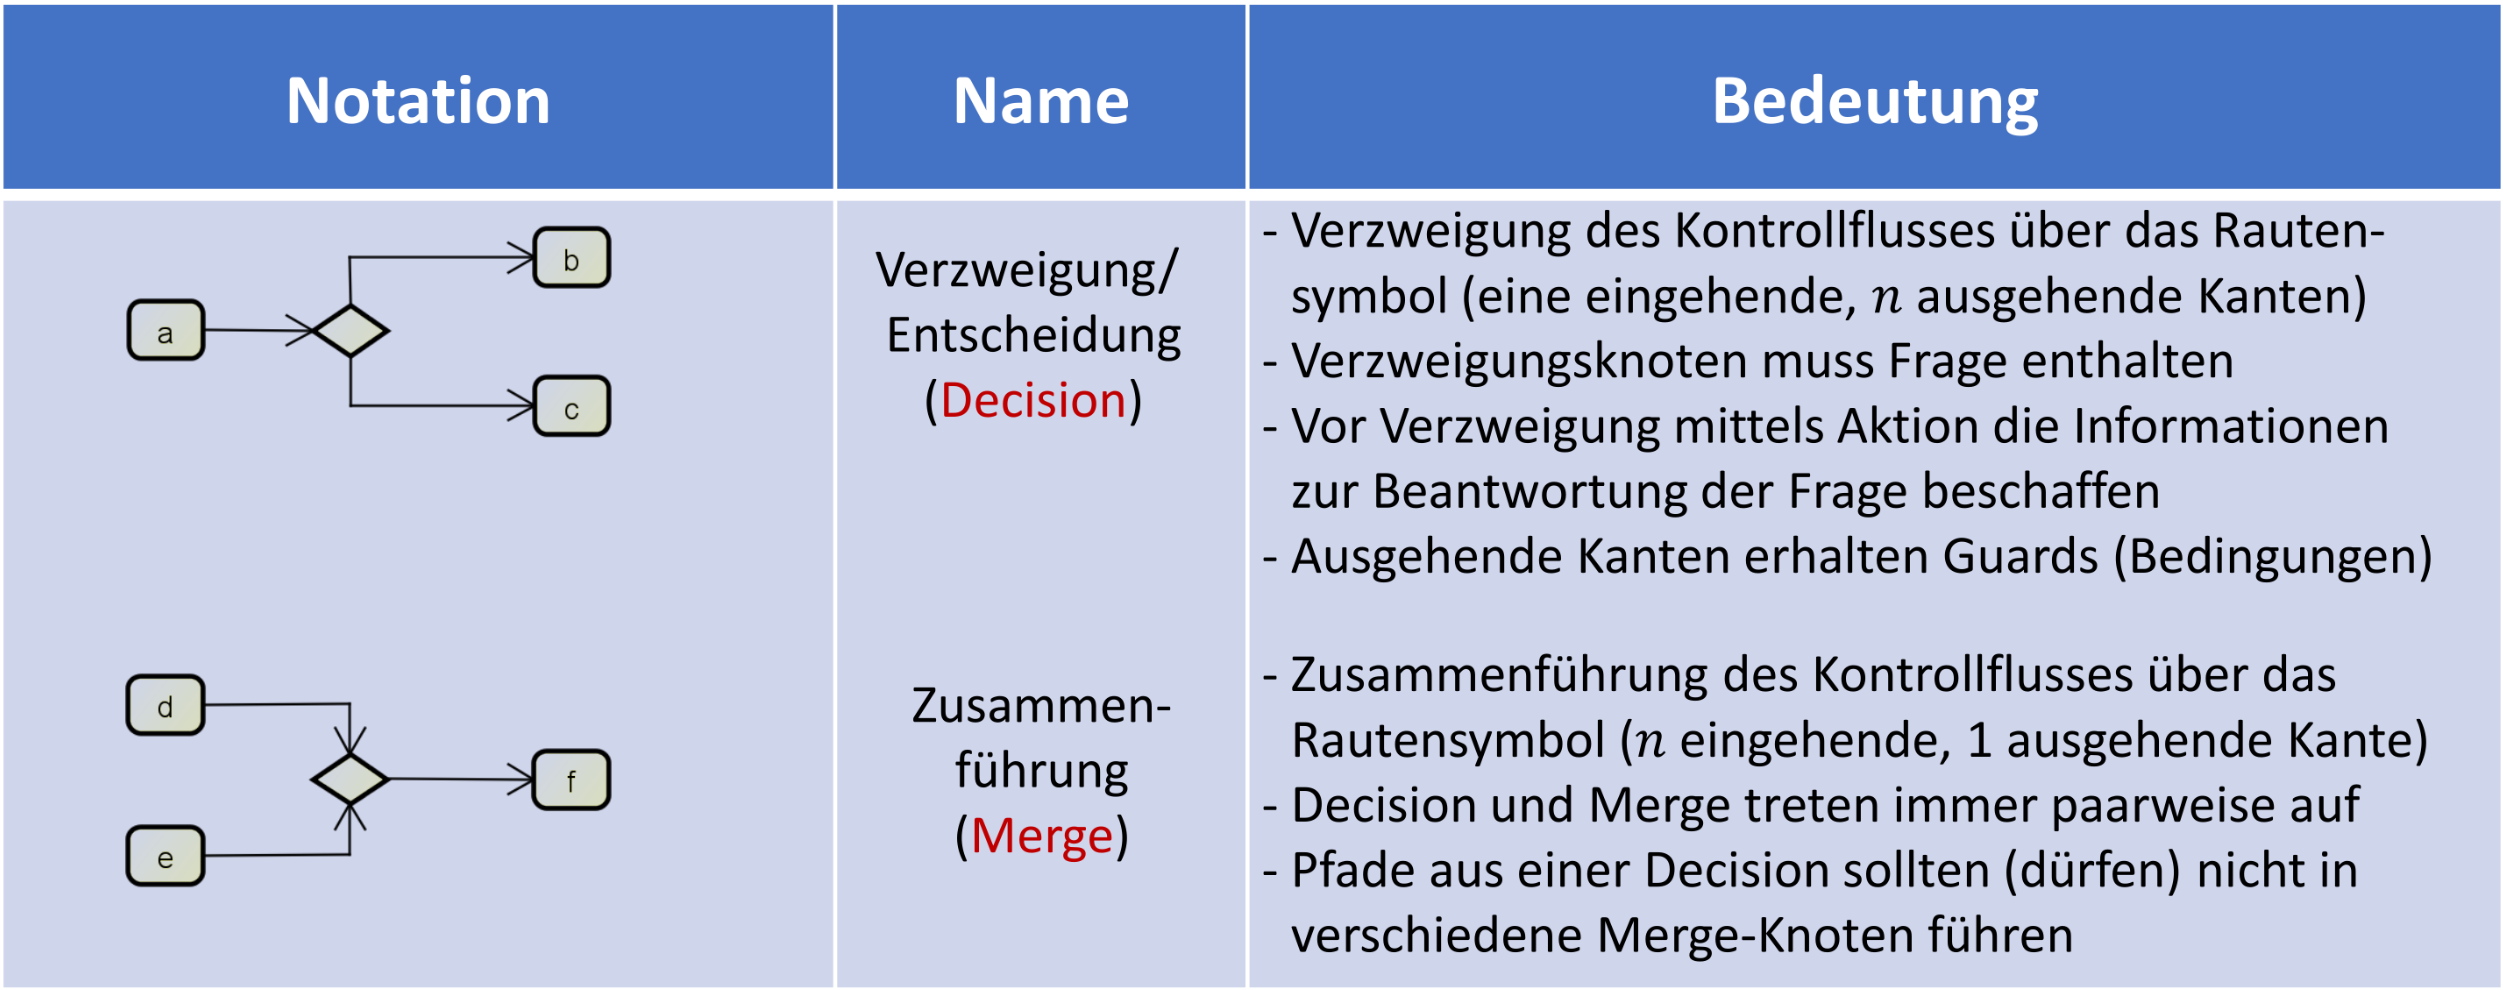
\includegraphics[width=0.75\textwidth]{Aktivitaet-Tabellen/2.png}

\vspace{1em}

\centering

\includegraphics[width=0.75\textwidth]{Aktivitaet-Tabellen/3.png}

\vspace{1em}

\centering
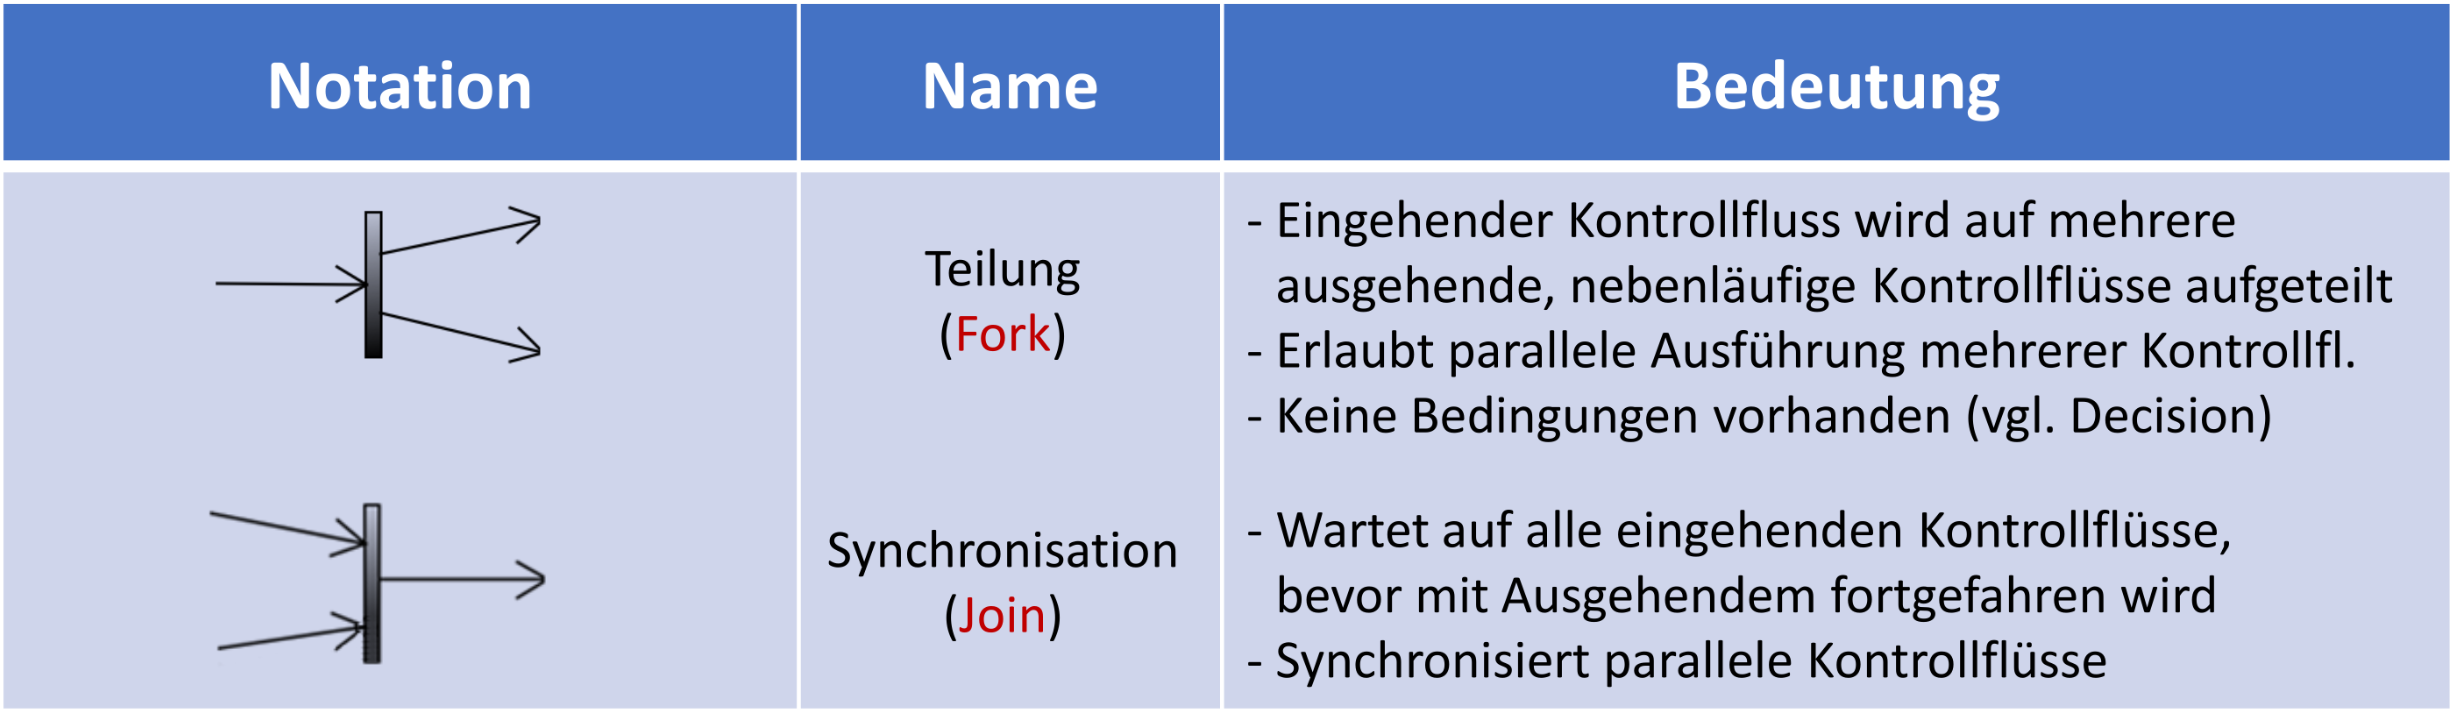
\includegraphics[width=0.75\textwidth]{Aktivitaet-Tabellen/4.png}

\vspace{1em}

\centering
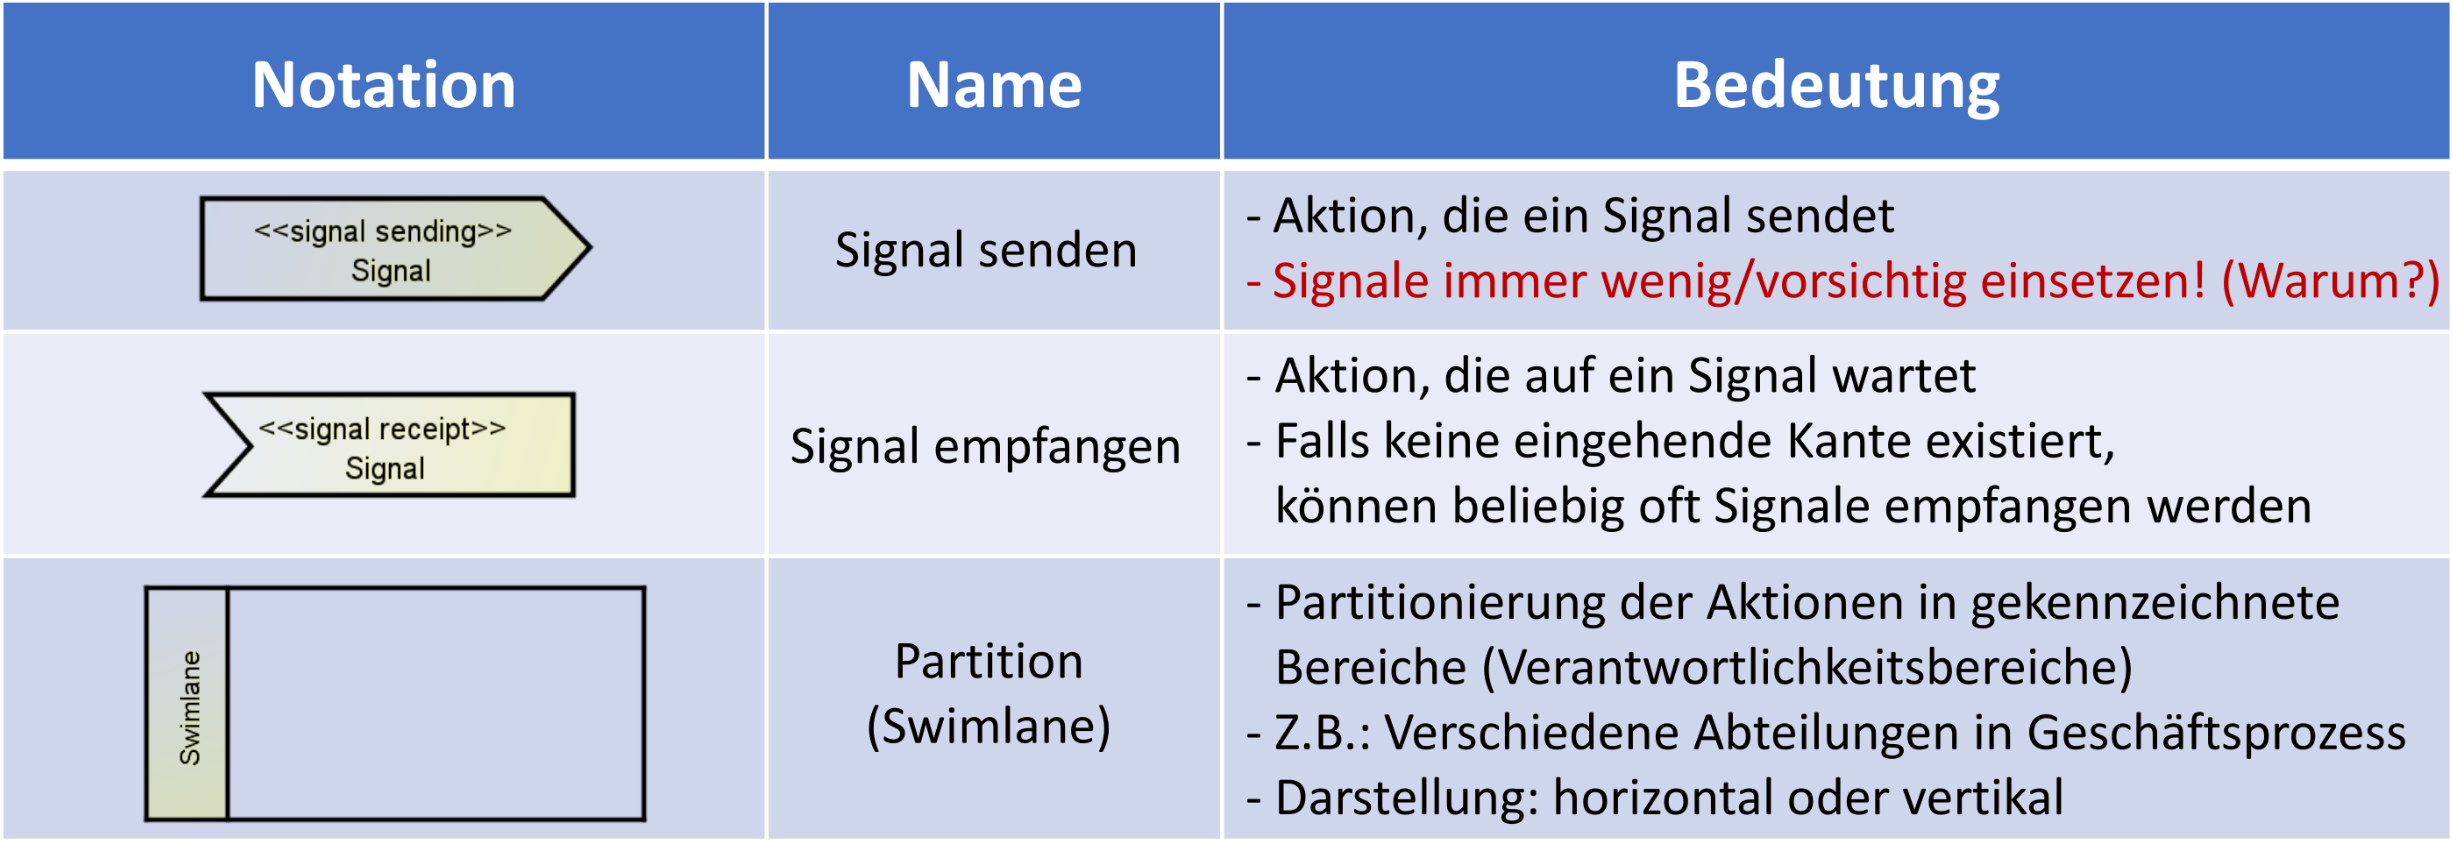
\includegraphics[width=0.75\textwidth]{Aktivitaet-Tabellen/5.png}

\newpage

\raggedright \subsection{Zustandsdiagramme}

\textbf{Zustandsdiagramme beantworten die Frage:} “Wie verhält sich System in bestimmtem Zustand bei gewissen Ereignissen?”

\vspace{1em}

\begin{figure}[ht]
    \centering
    \begin{minipage}[h]{0.45\textwidth}
        \raggedright
        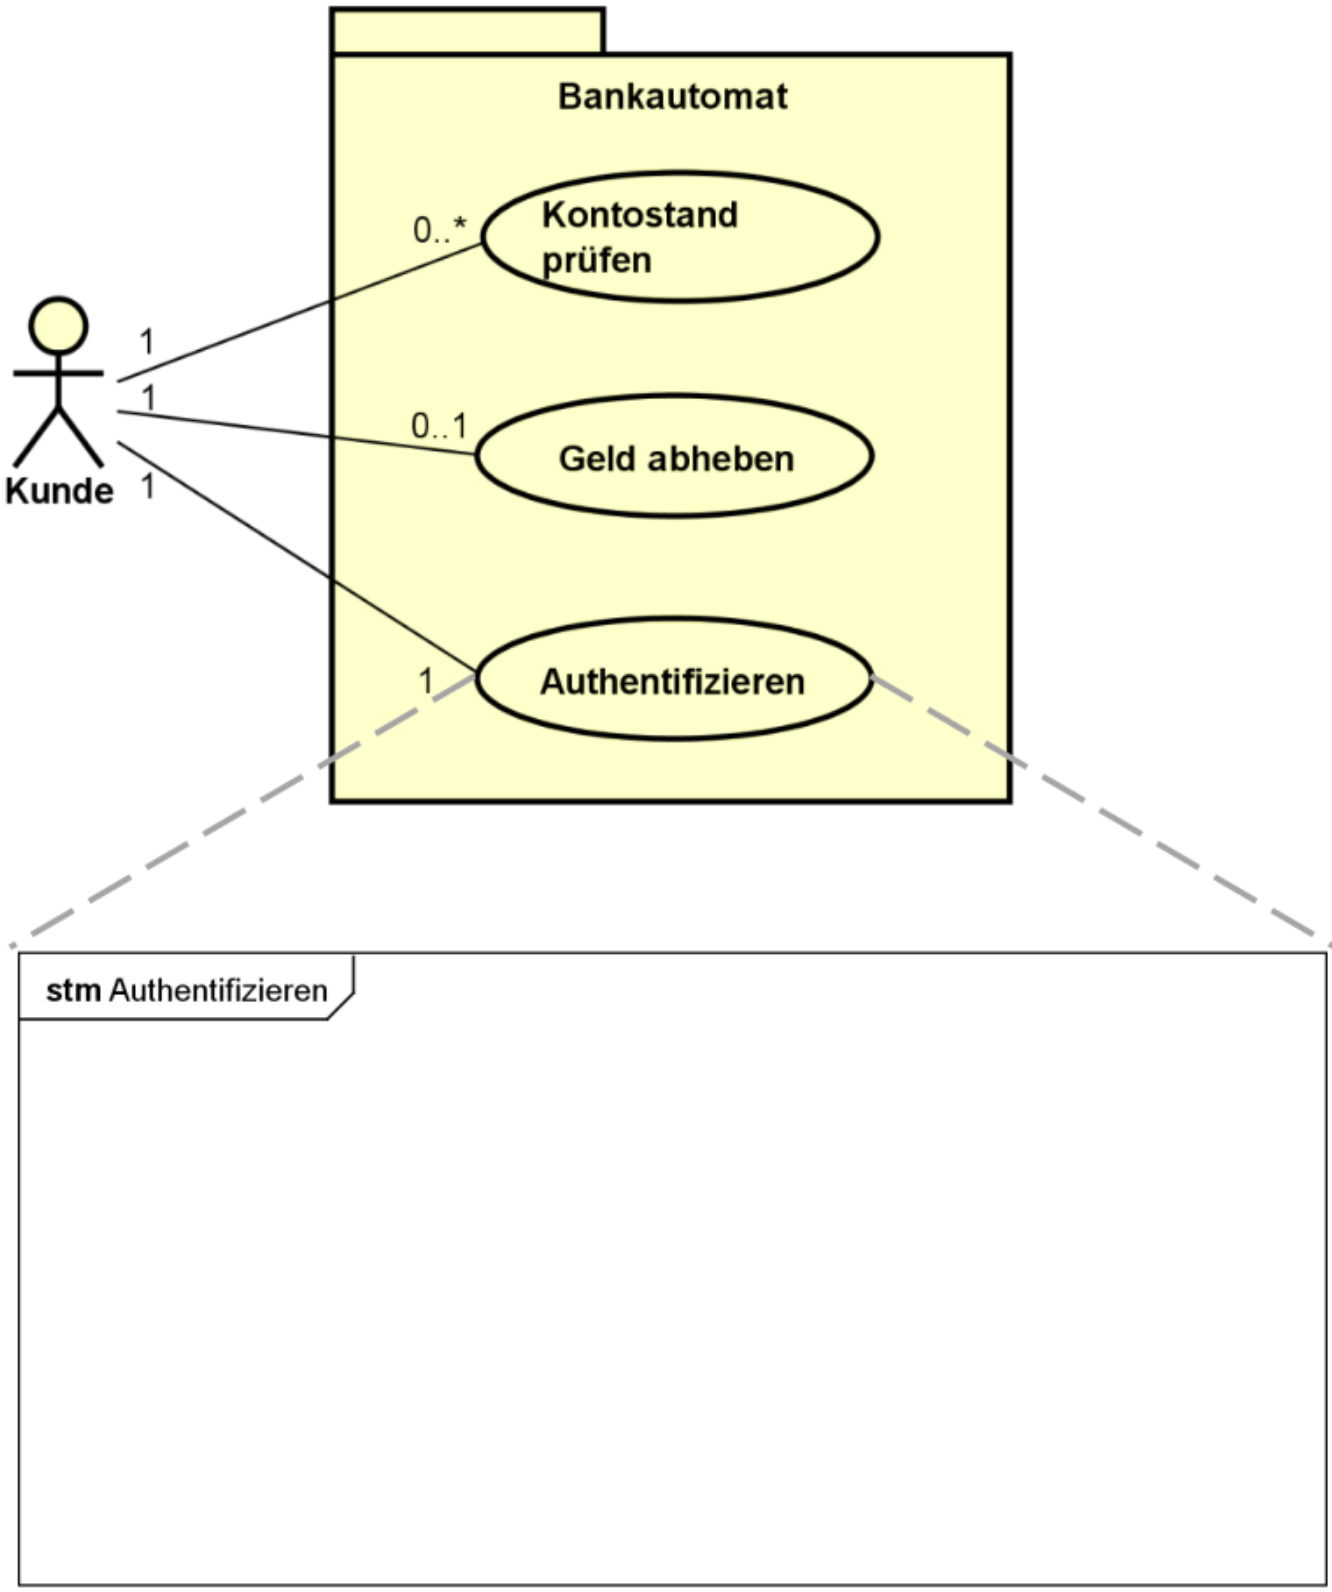
\includegraphics[width=0.7\textwidth]{Zustand-00.png}
    \end{minipage}
    \centering
    \begin{minipage}[h]{0.45\textwidth}
        \scriptsize
        \begin{itemize}
            \item \textbf{entry/:} Aktivitäten bei Eintritt in Zustand
            \item \textbf{do/:} Aktivitäten während Aufenthalt im Zustand
            \item \textbf{exit/:} Aktivitäten bei Verlassen des Zustandes
        \end{itemize}
        \centering
        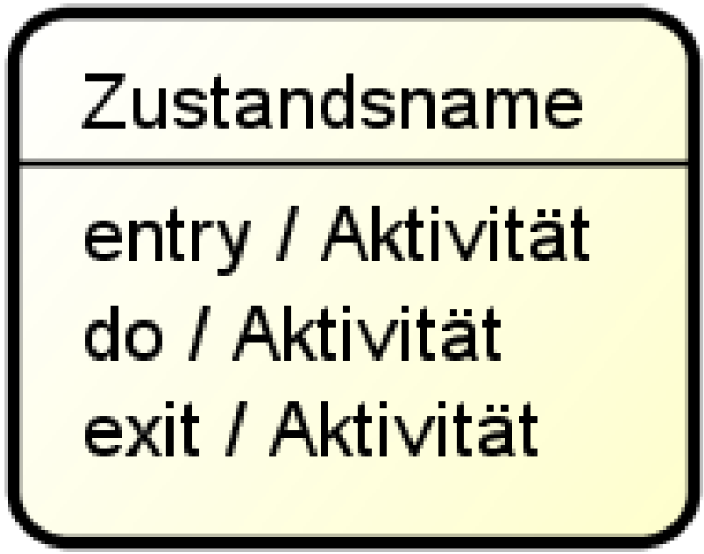
\includegraphics[width=0.3\textwidth]{Zustand-Elemente/0.png}
    \end{minipage}
\end{figure}



\subsubsection{Elemente}

\vspace{1em}

\centering Zustandsübergang \\
\vspace{1em}
\centering 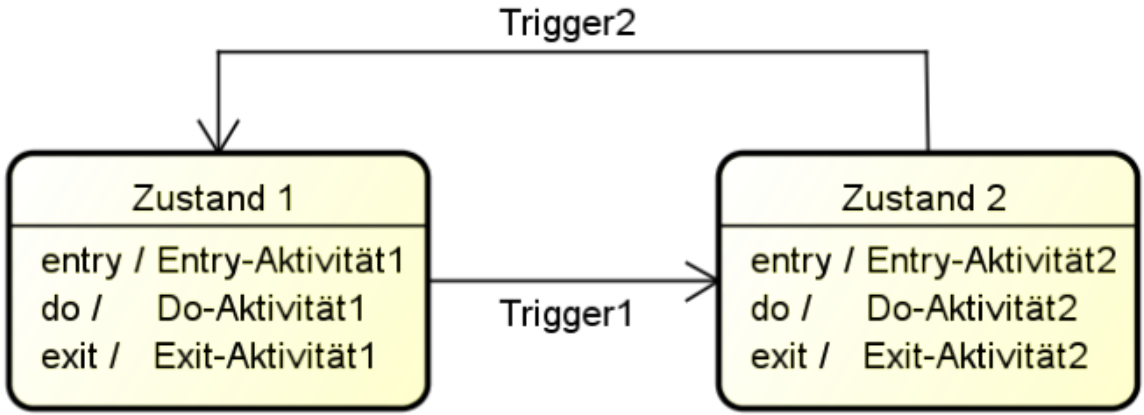
\includegraphics[width=0.4\textwidth]{Zustand-Elemente/1.png}

\vspace{1em}

\begin{figure}[ht]
    \centering
    \begin{minipage}[t]{0.30\textwidth}
        \centering Startzustand \\
        \vspace{1em}
        \centering 
\includegraphics[width=0.2\textwidth]{Zustand-Elemente/2.png}
    \end{minipage}
    \centering
    \begin{minipage}[t]{0.30\textwidth}
        \centering Endzustand \\
        \vspace{1em}
        \centering 
\includegraphics[width=0.2\textwidth]{Zustand-Elemente/3.png}
    \end{minipage}
    \centering
    \begin{minipage}[t]{0.30\textwidth}
        \centering Terminator \\
        \vspace{1em}
        \centering 
\includegraphics[width=0.2\textwidth]{Zustand-Elemente/4.png}
    \end{minipage}
\end{figure}

\vspace{1em}

\begin{figure}[ht]
    \centering
    \begin{minipage}[t]{0.30\textwidth}
        \centering Entscheidung \\
        \vspace{1em}
        \centering 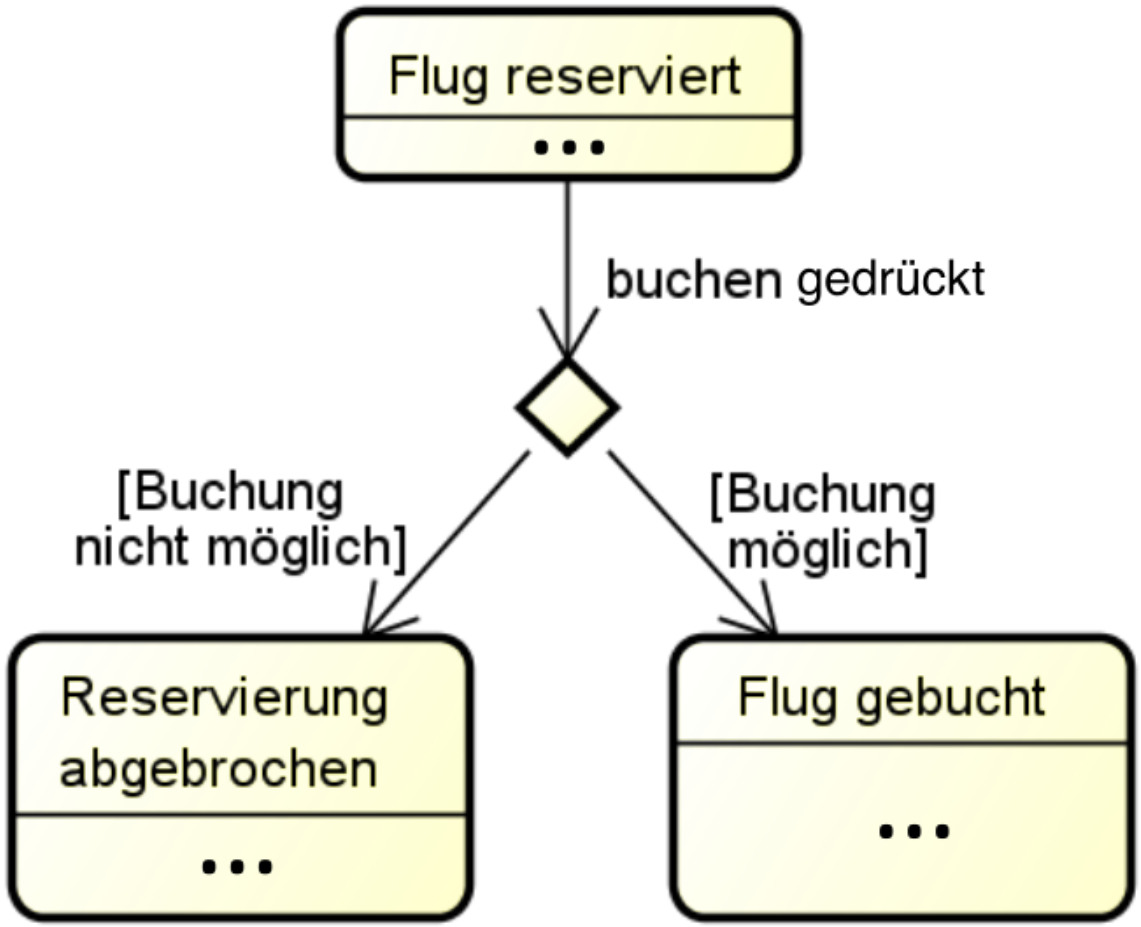
\includegraphics[width=0.9\textwidth]{Zustand-Elemente/5.png}
    \end{minipage}
    \centering
    \begin{minipage}[t]{0.30\textwidth}
        \centering Kreuzung/Verbindung \\
        \vspace{1em}
        \centering 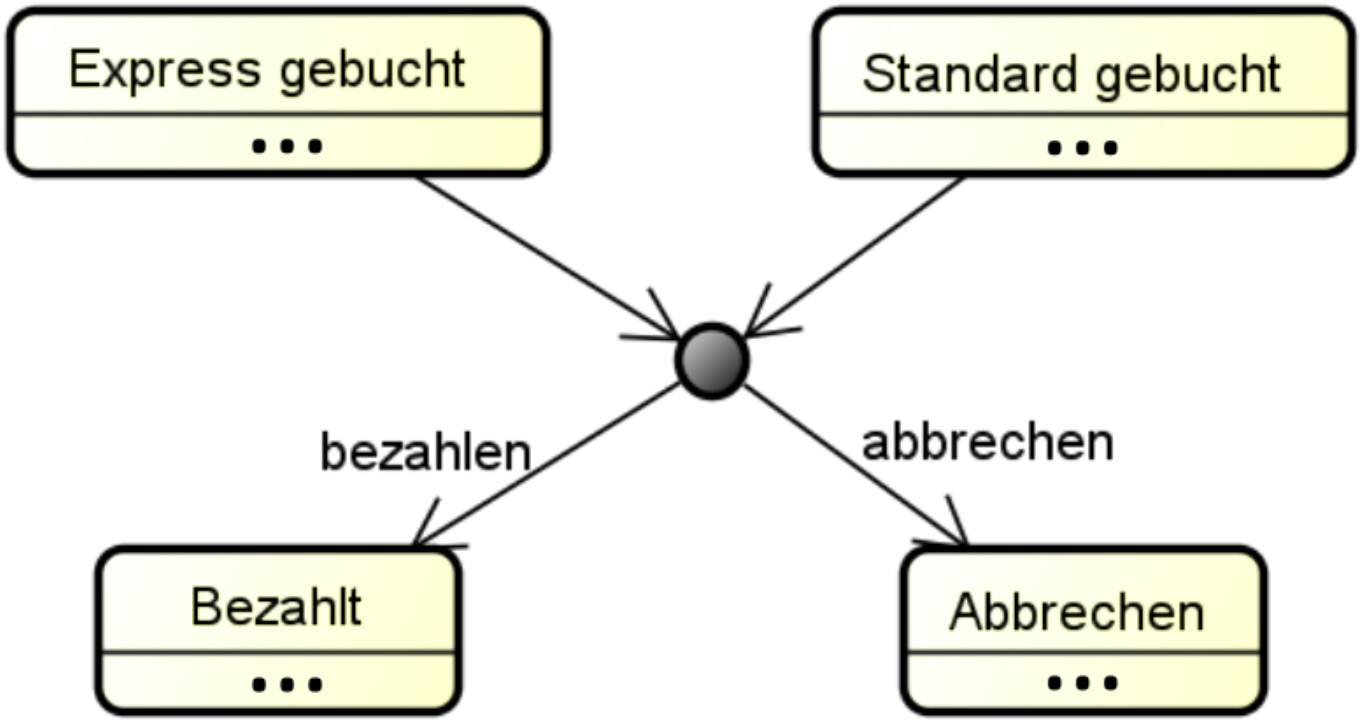
\includegraphics[width=0.9\textwidth]{Zustand-Elemente/6.png}
    \end{minipage}
    \centering
    \begin{minipage}[t]{0.30\textwidth}
        \centering Teilung und Synchronisation \\
        \vspace{1em}
        \centering 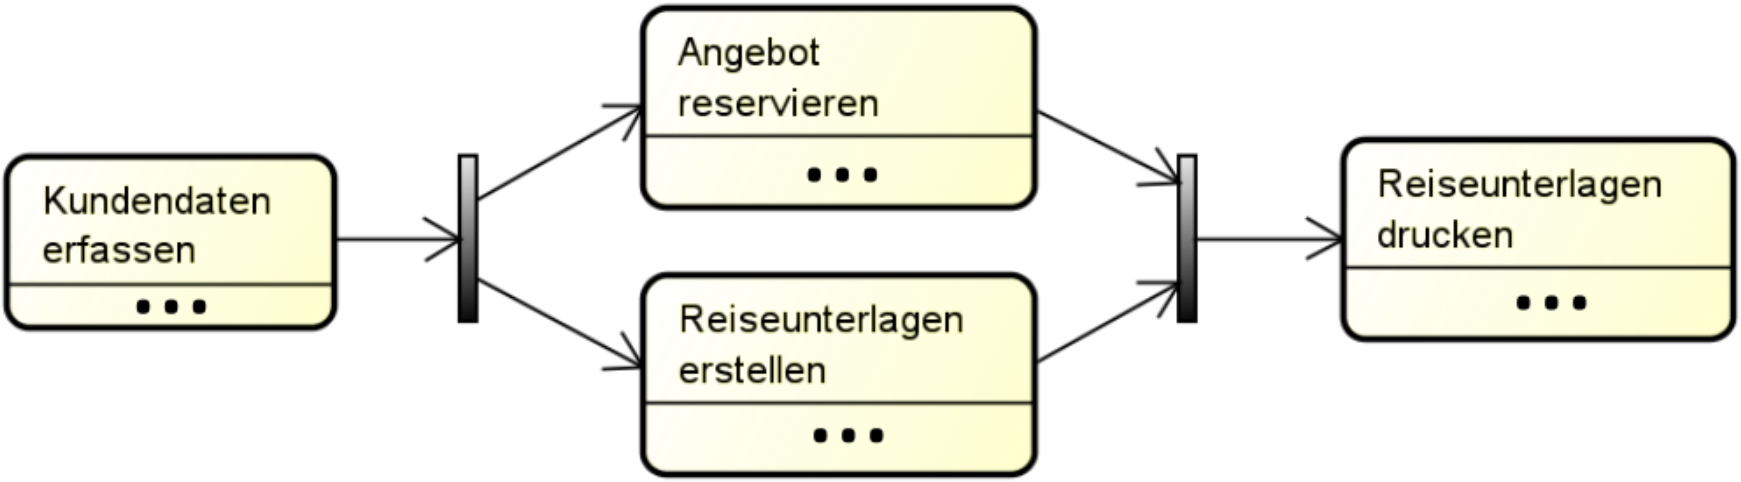
\includegraphics[width=0.9\textwidth]{Zustand-Elemente/7.png}
    \end{minipage}
\end{figure}



\raggedright \subsection{Paketdiagramme}

\begin{itemize}
    \item \textbf{Problem:} In großen Softwaresystemen ist es schwer den Überblick zu behalten
    \begin{itemize}
        \item \textit{Es existieren meist hunderte von Use Cases, Aktivitätsdiagramme, Klassen etc.}
    \end{itemize}
    \item \textbf{Ziel:} Auf hoher Ebene Struktur in die Systembeschreibung bringen
    \item \textbf{Lösung:} Einteilung des Systems in Pakete (Abstraktion)
\end{itemize}

\textbf{Paketdiagramme benatworten die Frage:} “Wie kann ich mein System so aufteilen und darstellen, dass ich den Überblick behalte?”

\begin{itemize}
    \item Paket bündelt Elemente der UML sinnvoll, d.h. nach einem Zusammenhang
    \item Paket entspricht einem in sich geschlossenen Teilsystem
    \item Pakete können hierarchisch geschachtelt sein (ein Paket enthält Pakete)
\end{itemize}

\begin{figure}[ht]
    \centering
    \begin{minipage}[t]{0.45\textwidth}
        \centering Funktionale Gliederung \\
        \vspace{1em}
        \centering 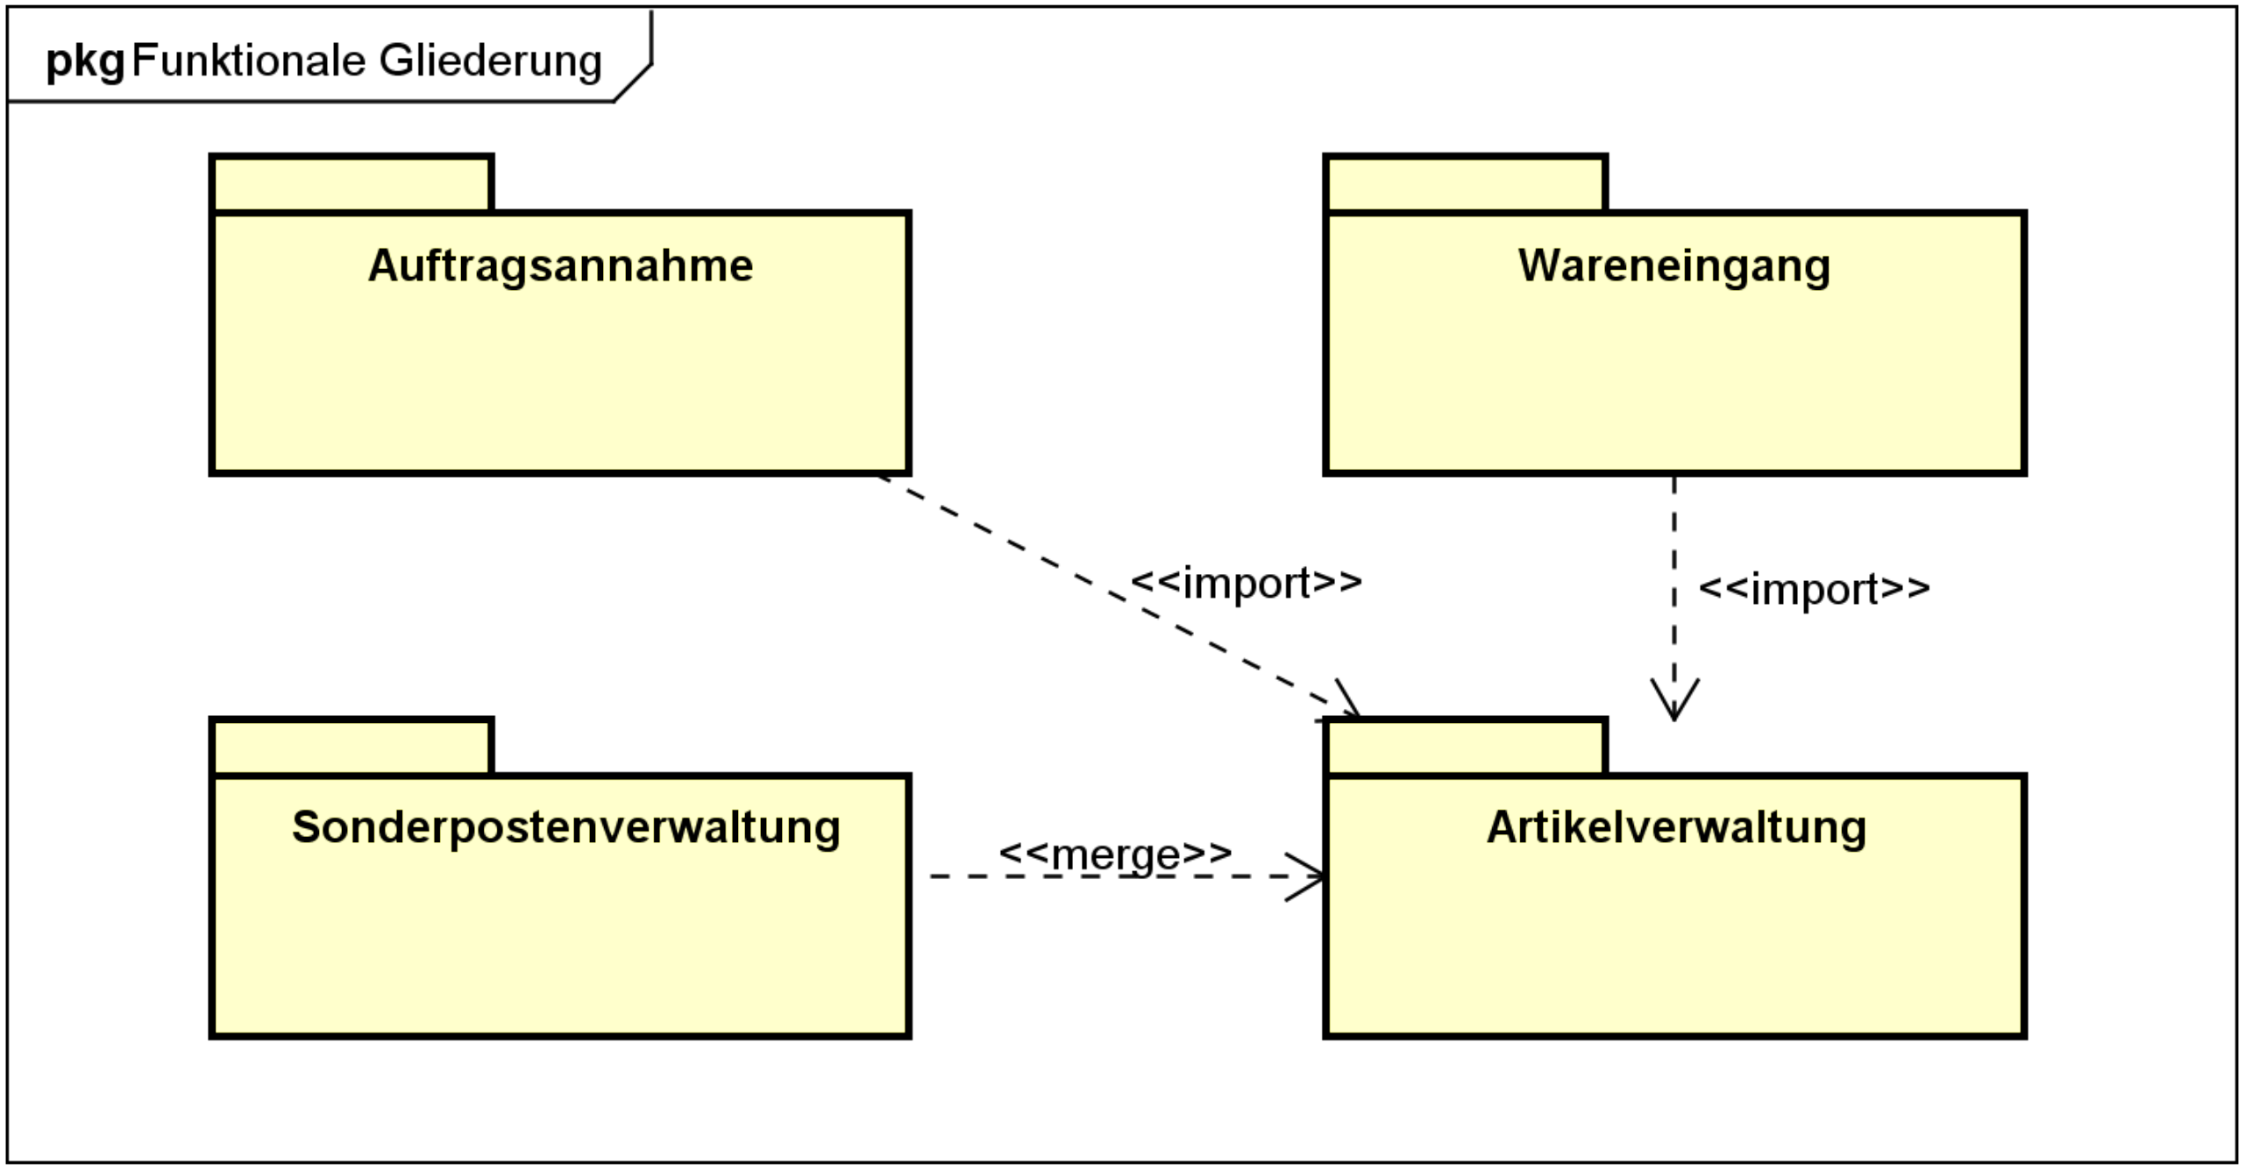
\includegraphics[width=0.9\textwidth]{Paket-00.png}
    \end{minipage}
    \centering
    \begin{minipage}[t]{0.45\textwidth}
        \centering Gliederung in Schichten \\
        \vspace{1em}
        \centering 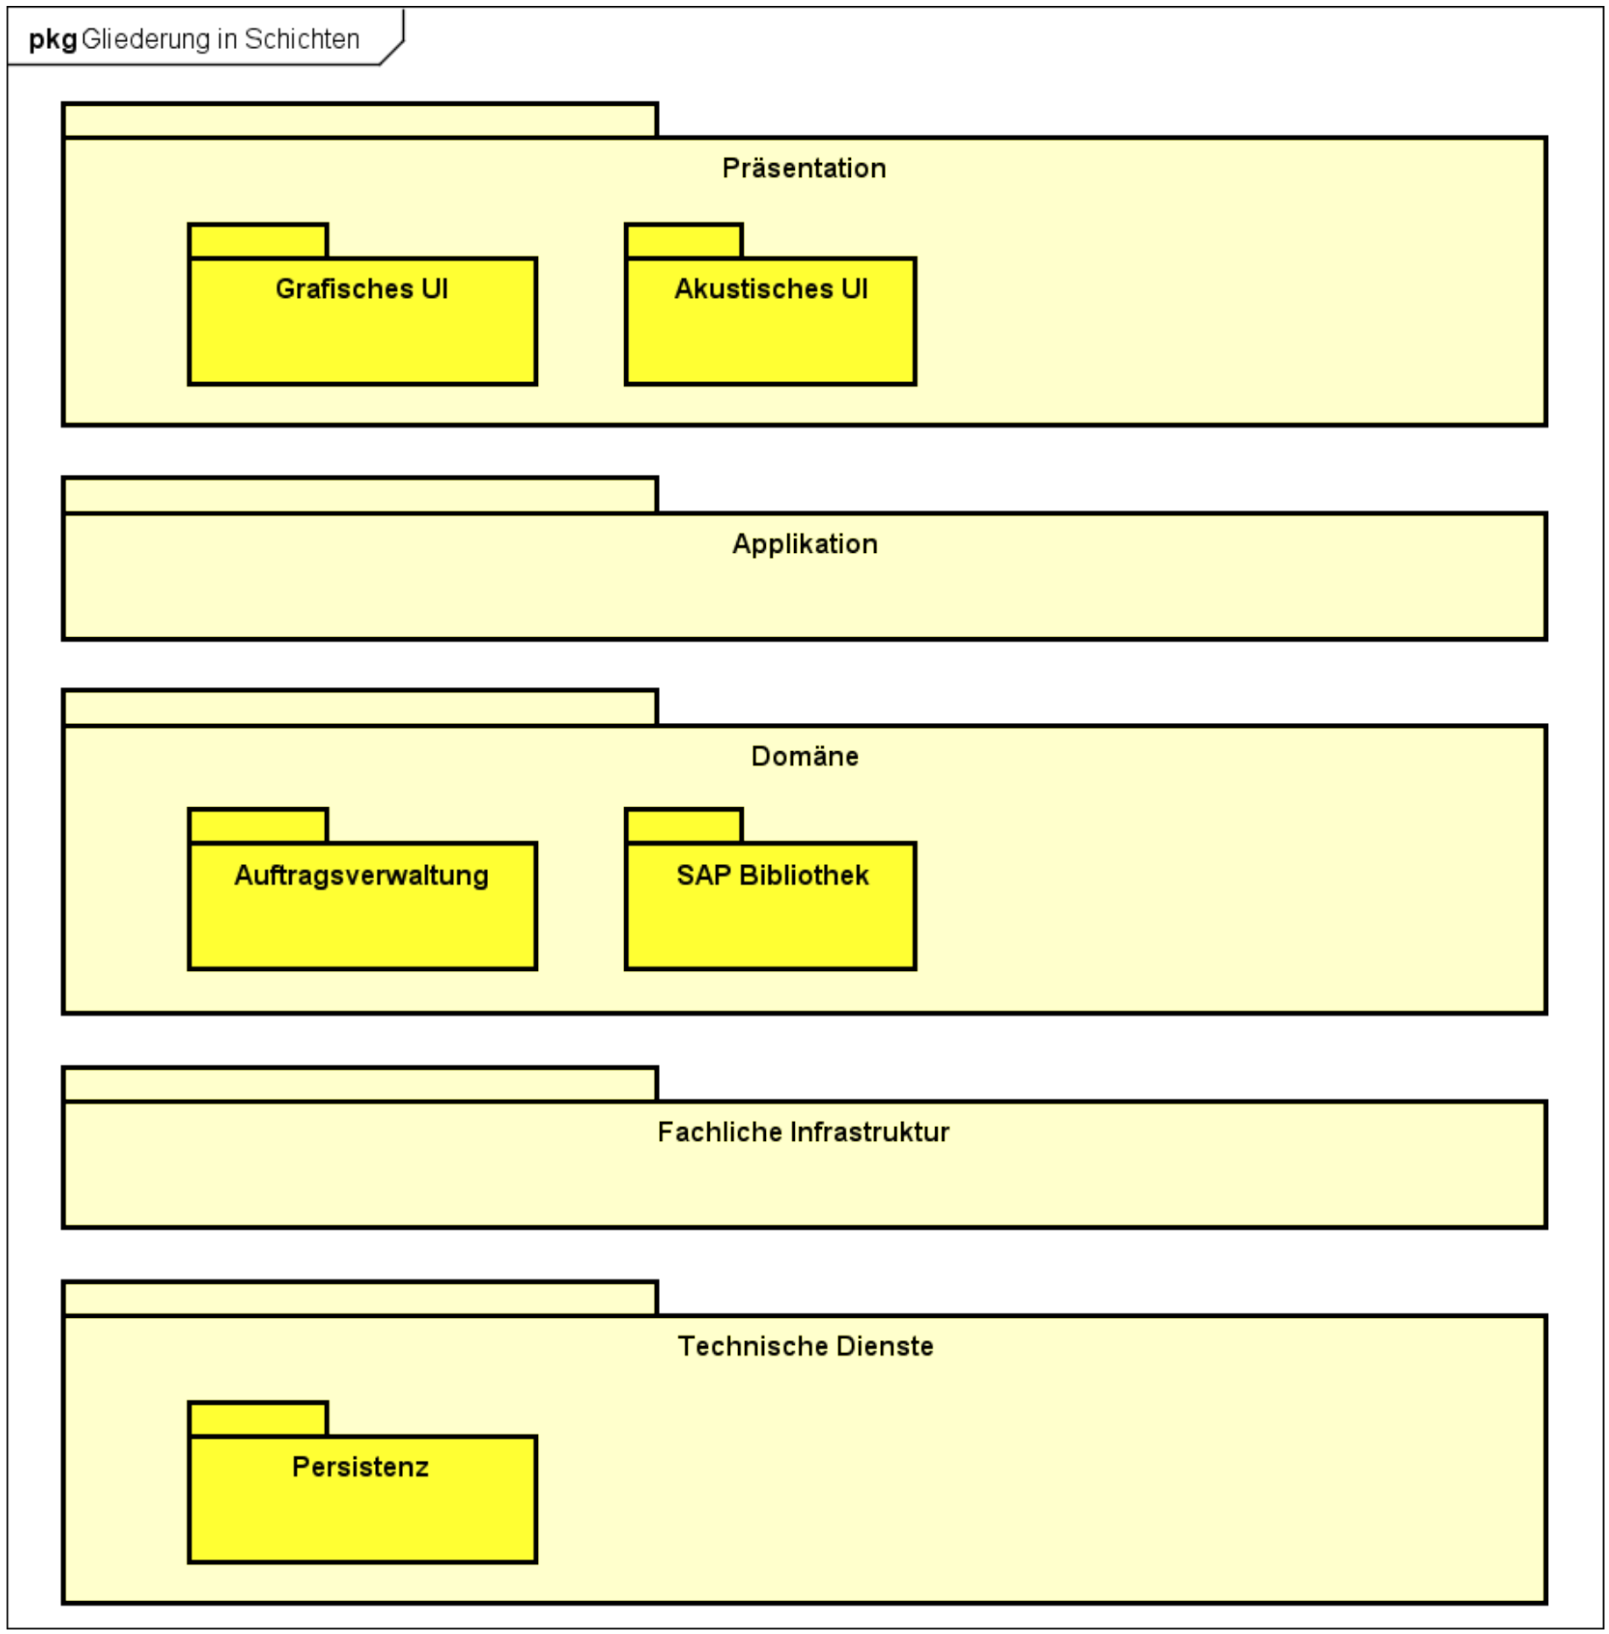
\includegraphics[width=0.9\textwidth]{Paket-01.png}
    \end{minipage}
\end{figure}

\subsubsection{Elemente und Notation}

\centering 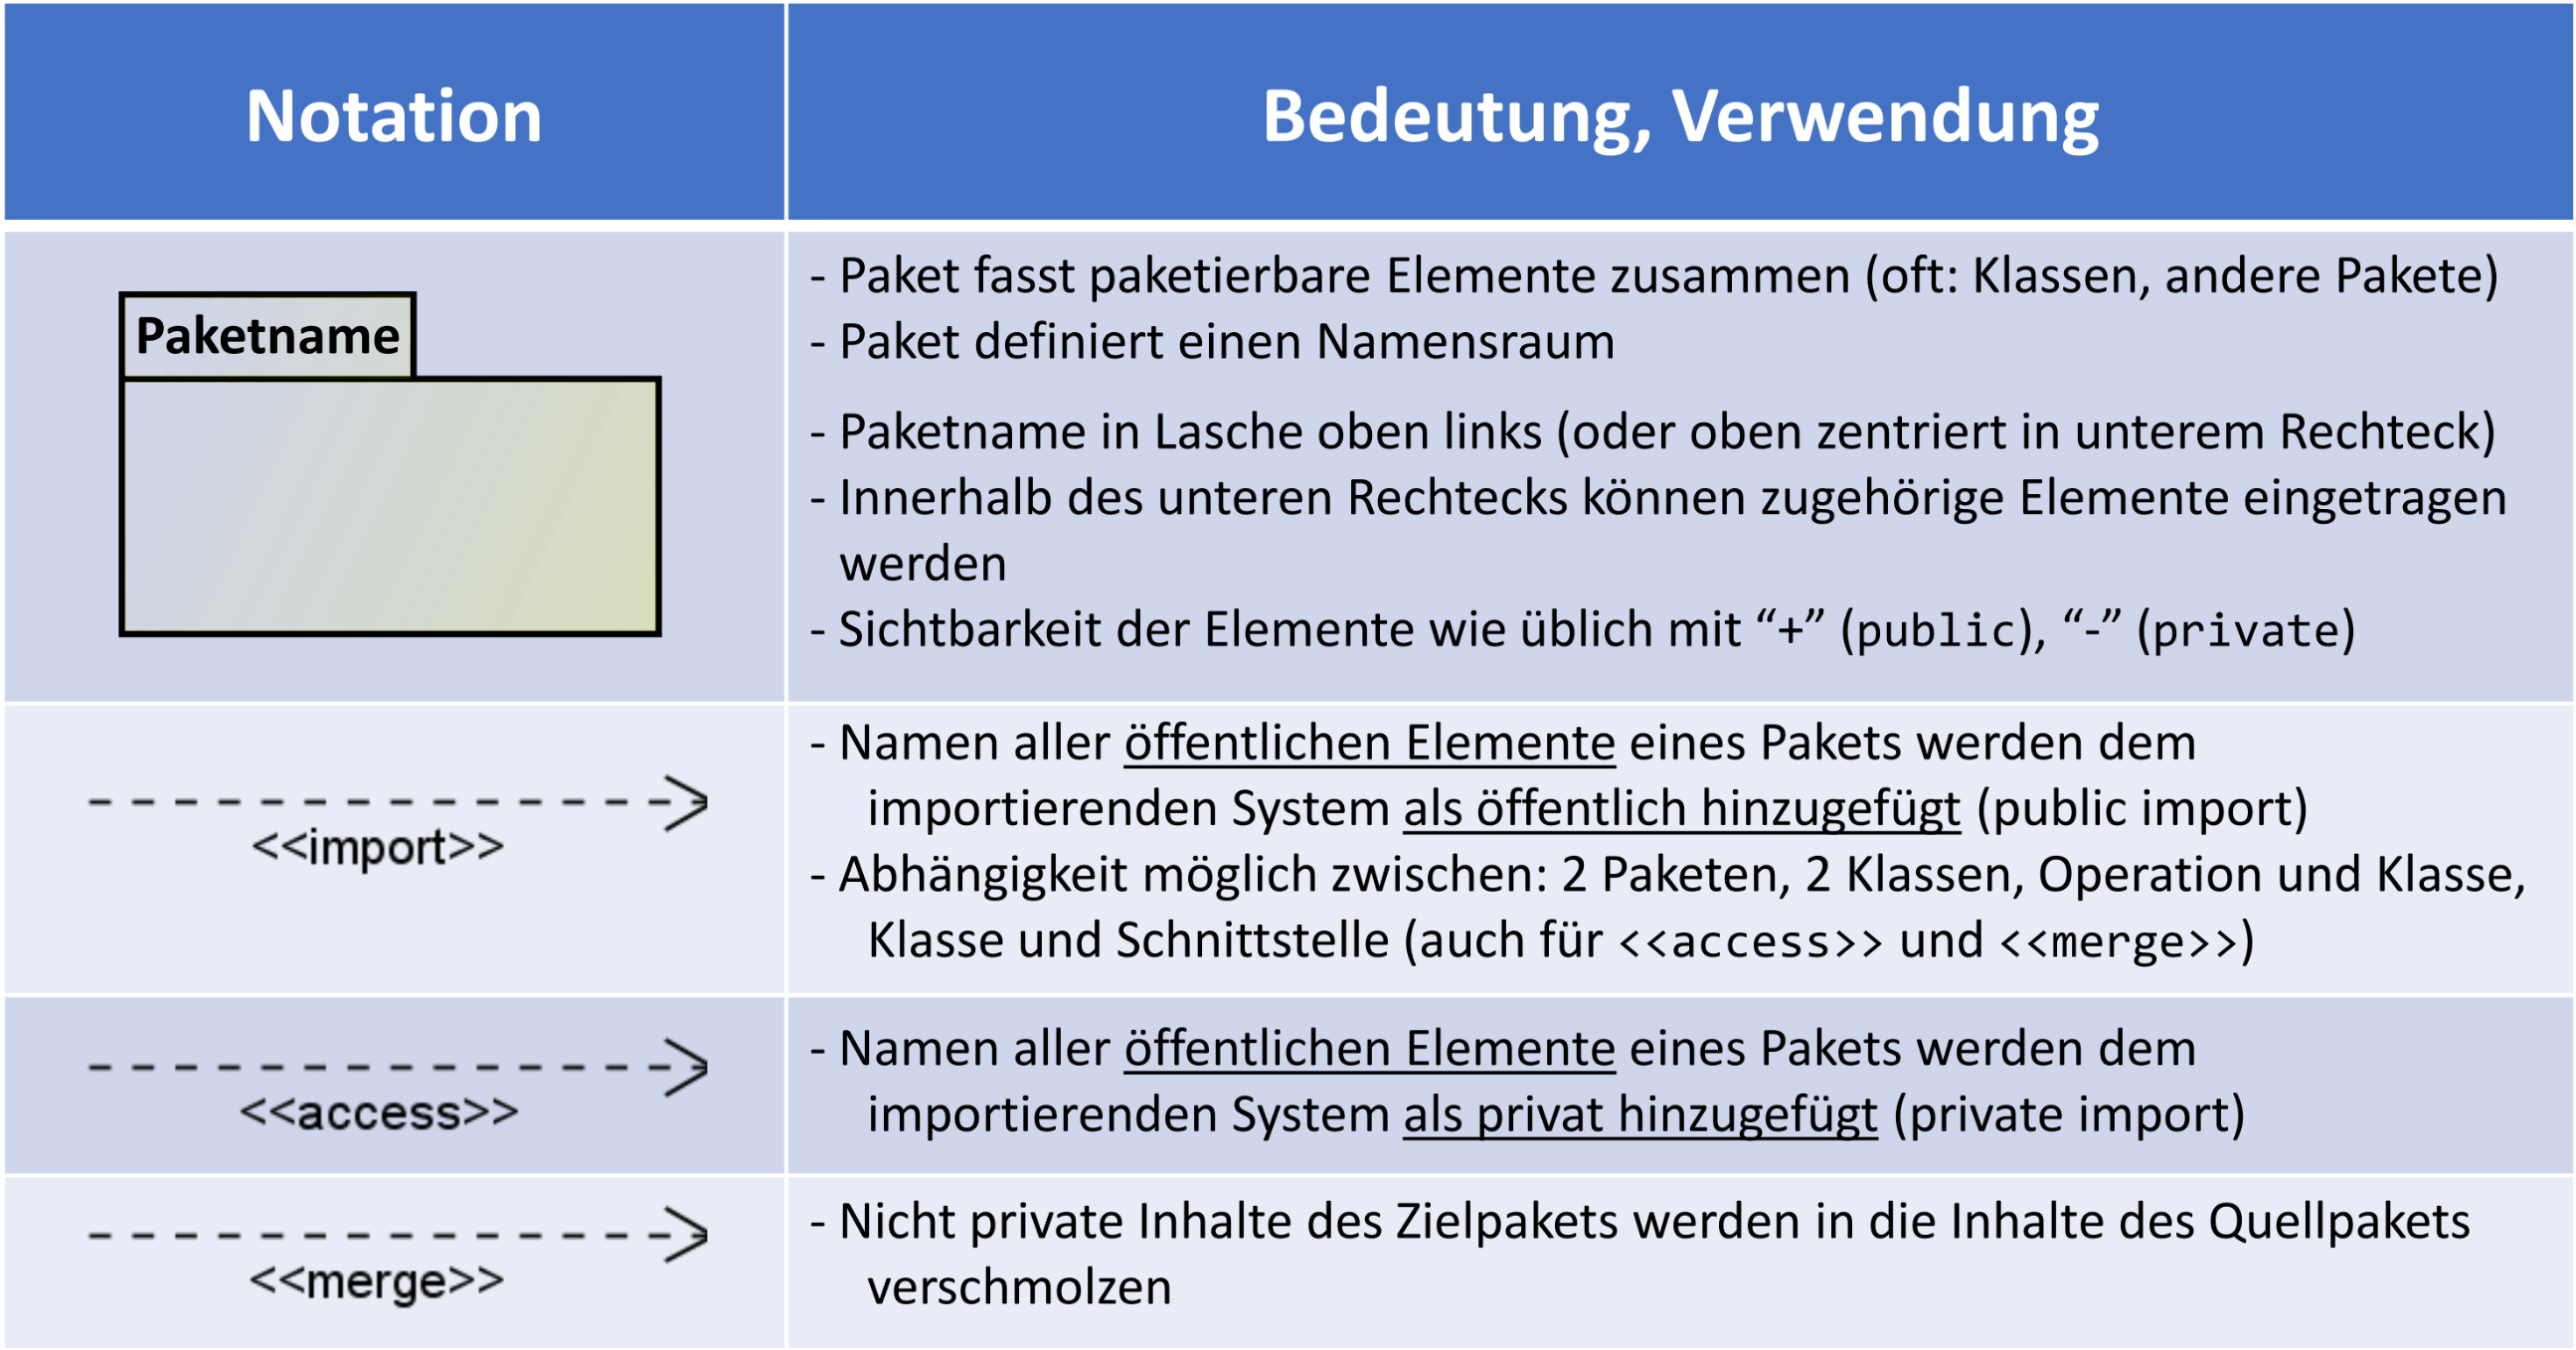
\includegraphics[width=0.8\textwidth]{Paket-03.png}


\newpage

\raggedright \subsection{Klassendiagramm}

\vspace{1em}

\raggedright \subsubsection{Definition der Klassen}

\vspace{1em}

\begin{figure}[ht]
    \centering
    \begin{minipage}[h]{0.45\textwidth}
        \centering 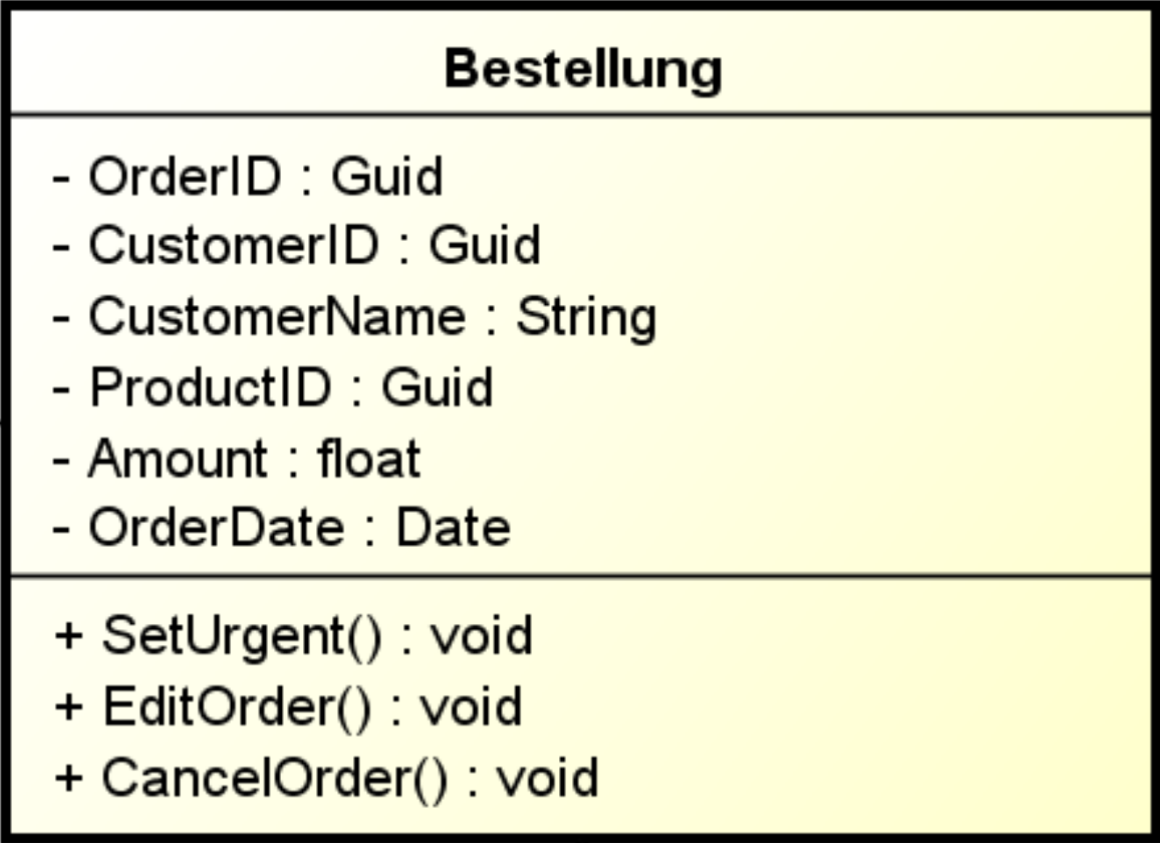
\includegraphics[width=0.6\textwidth]{Klassen-00.png}
    \end{minipage}
    \centering
    \begin{minipage}[h]{0.45\textwidth}
        \raggedright \small
        \begin{itemize}
            \item + : \textit{public} \\ Öffentlich; für alle Elemente sichtbar
            \item $\sim$ : \textit{package} \\ Sichtbar für alle Elemente im gleichen Paket
            \item \# : \textit{protected} \\ Sichtbar für Instanzen und Instanzen abgeleiteter Klassen
            \item --- : \textit{private} \\ Sichtbar nur für Instanzen dieser Klasse
        \end{itemize}
    \end{minipage}
\end{figure}


\raggedright \subsubsection{Vererbung}

\vspace{1em}

\begin{minipage}[h]{0.3\textwidth}
    \raggedleft 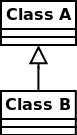
\includegraphics[width=0.3\textwidth]{Klassen-Elemente/1.png} 
\end{minipage}
\begin{minipage}[h]{0.65\textwidth}
    \begin{itemize}
        \item Tiger ist ein Raubtier
        \item Auto ist ein Fortbewegungsmittel
        \item Auto ist ein Luxusgut
    \end{itemize}
\end{minipage}

\vspace{1em}

\raggedright \subsubsection{Assoziation}

\vspace{1em}

\begin{minipage}[h]{0.3\textwidth}
    \raggedleft 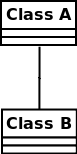
\includegraphics[width=0.3\textwidth]{Klassen-Elemente/2.png} 
\end{minipage}
\begin{minipage}[h]{0.65\textwidth}
    \begin{itemize}
        \item Person - Termin: Eine Person hat Termine; Termine gehören zu einer Person
        \item Lehrer - Schüler: Ein Schüler hat Lehrer; Lehrer haben Schüler
        \item Auto - Fahrer: Ein Auto hat einen Fahrer; ein Fahrer hat ein Auto
    \end{itemize}
\end{minipage}

\vspace{1em}

\raggedright \subsubsection{Aggregation}

\vspace{1em}

\begin{minipage}[h]{0.3\textwidth}
    \raggedleft 
\includegraphics[width=0.3\textwidth]{Klassen-Elemente/3.png} 
\end{minipage}
\begin{minipage}[h]{0.65\textwidth}
    \begin{itemize}
        \item PKW hat Räder
        \item Eltern haben Kinder
        \item Buchladen hat Bücher
    \end{itemize}
\end{minipage}

\vspace{1em}

\raggedright \subsubsection{Komposition}

\vspace{1em}

\begin{minipage}[h]{0.3\textwidth}
    \raggedleft 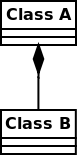
\includegraphics[width=0.3\textwidth]{Klassen-Elemente/4.png} 
\end{minipage}
\begin{minipage}[h]{0.65\textwidth}
    \begin{itemize}
        \item Buch hat Buchseiten (Buchseiten gibt es nicht ohne Buch)
        \item Rechnung hat Posten (Rechnungsposten gibt es nicht ohne Rechnung)
        \item Graph hat Knoten (Knoten gibt es nicht ohne Graph)
    \end{itemize}
\end{minipage}

\vspace{3em}

\raggedright \subsubsection*{Beispiel}

\vspace{1em}

\centering 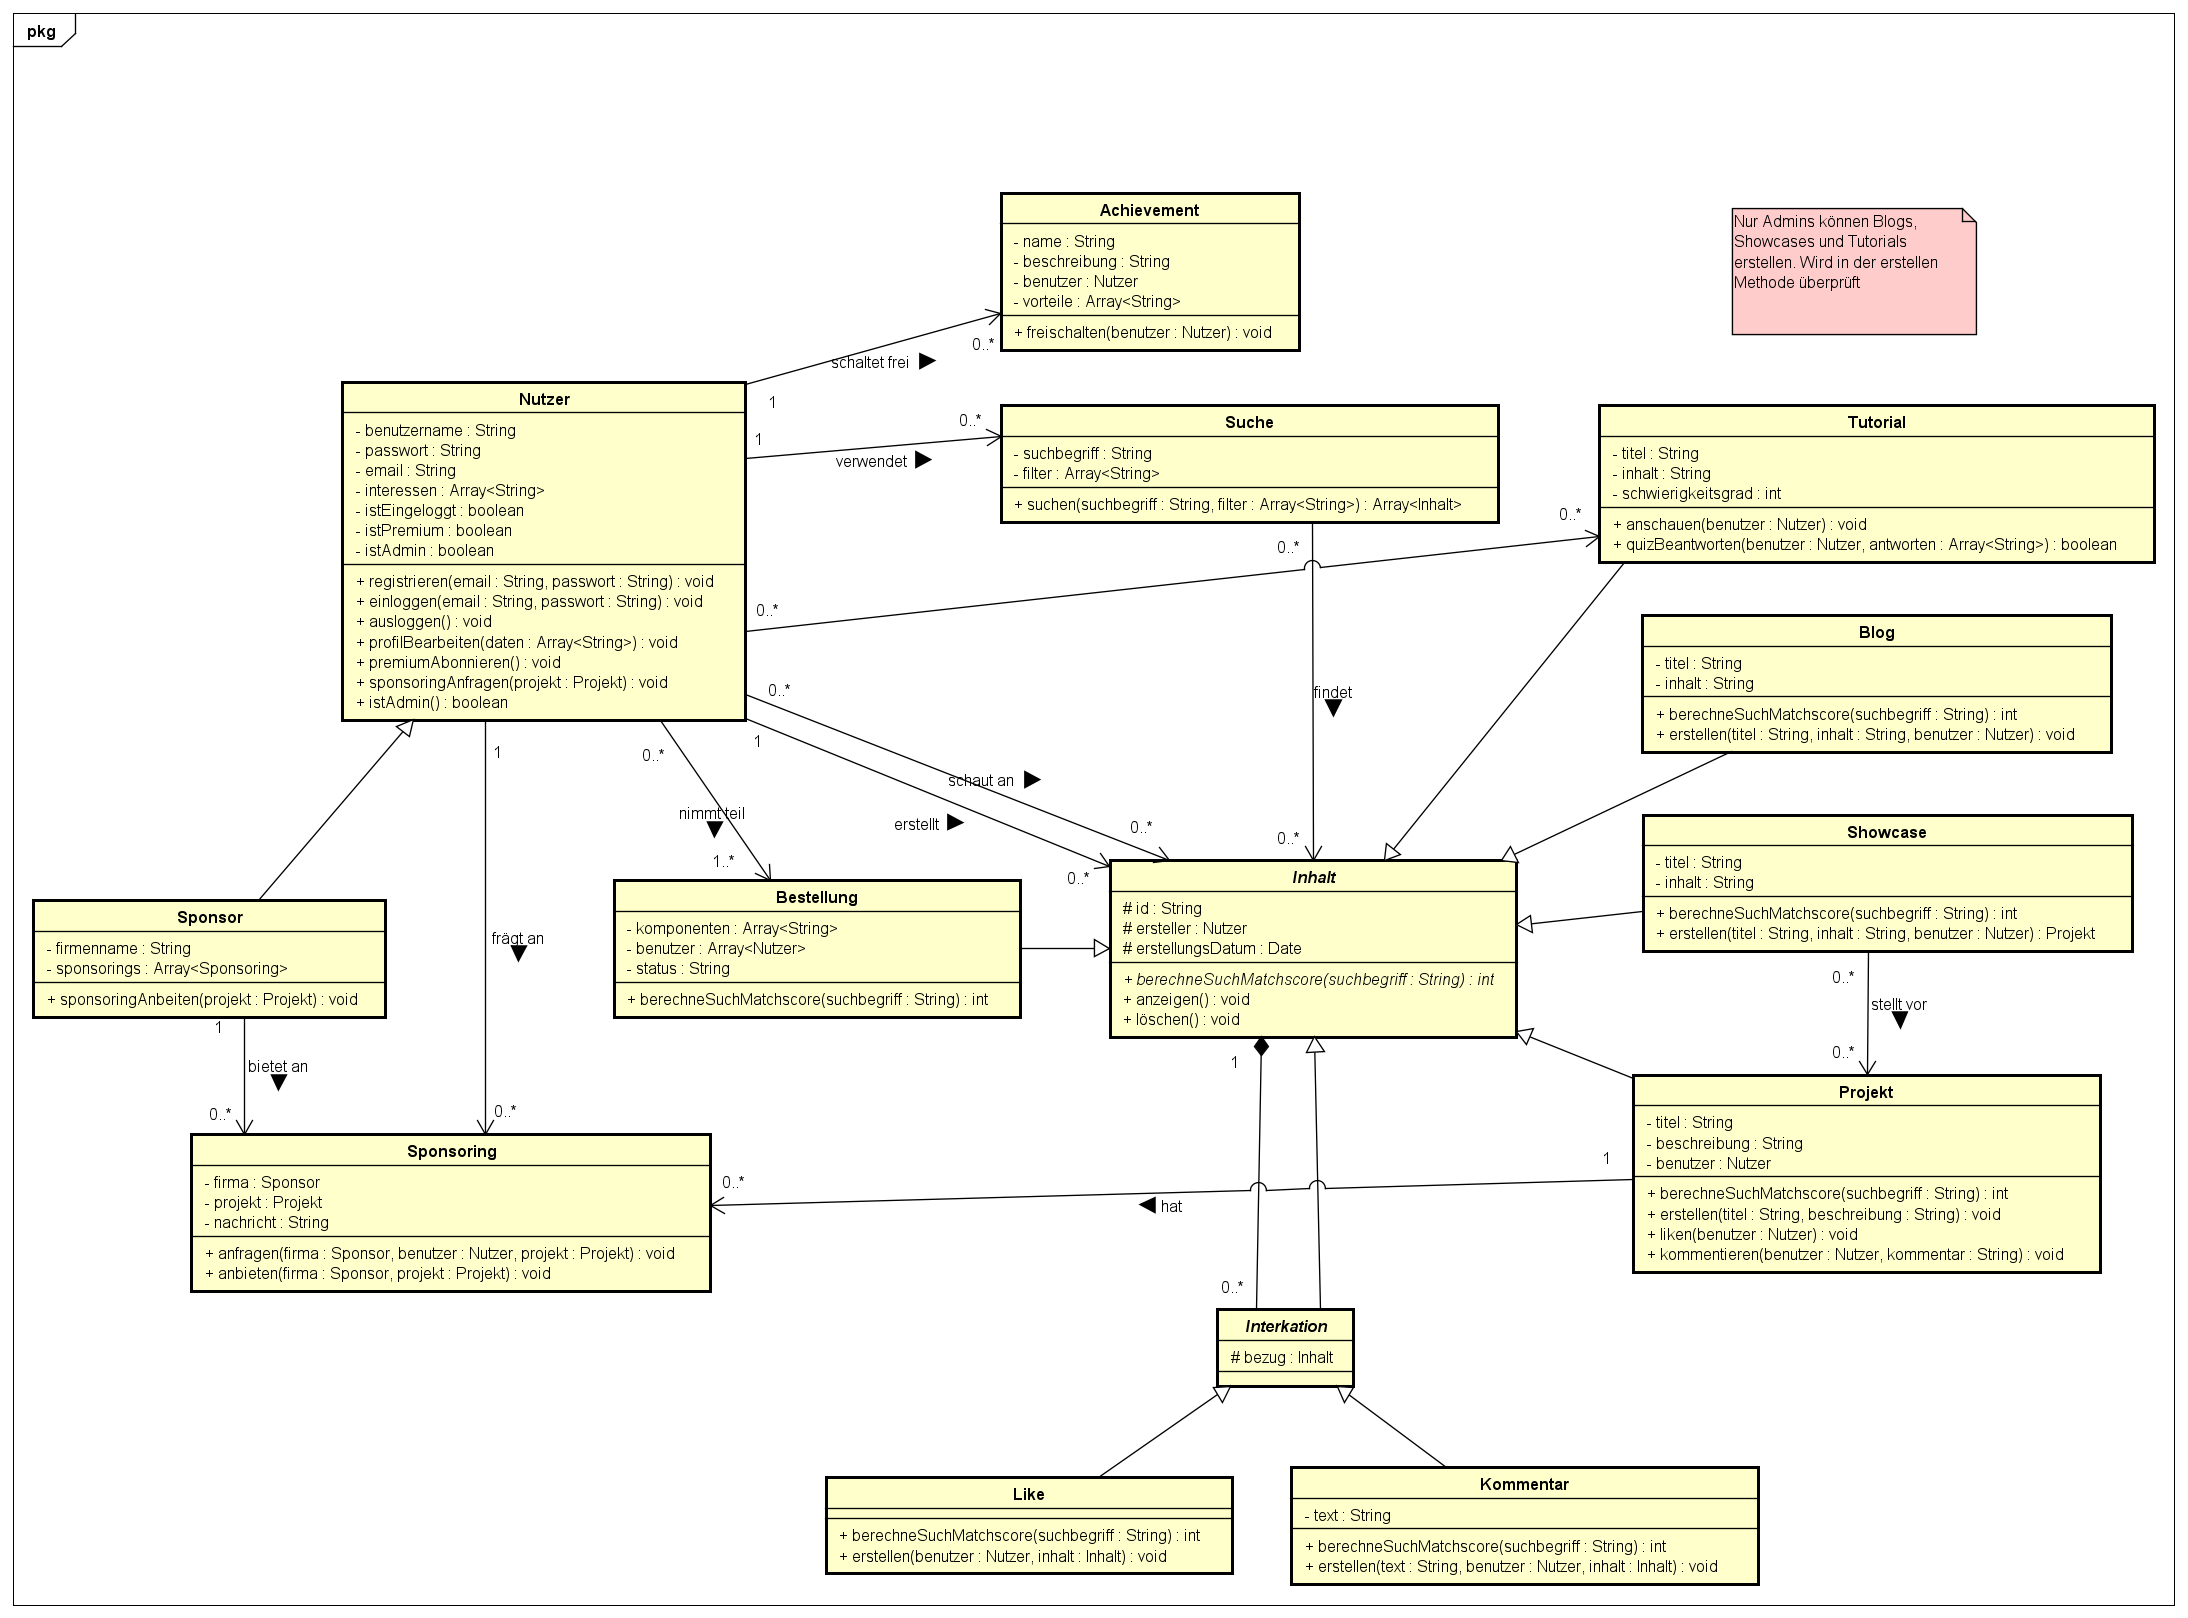
\includegraphics[width=1\textwidth]{Klassen-02.png}

\newpage



\raggedright \subsection{Objektdiagramme}

\textbf{Ziel:} Momentaufnahme des Systemzustandes darstellen

\vspace{2em}

\begin{minipage}[h]{0.45\textwidth}
    \tiny \centering Korrespondierende Elemente \\
    \vspace{1em}
    \centering 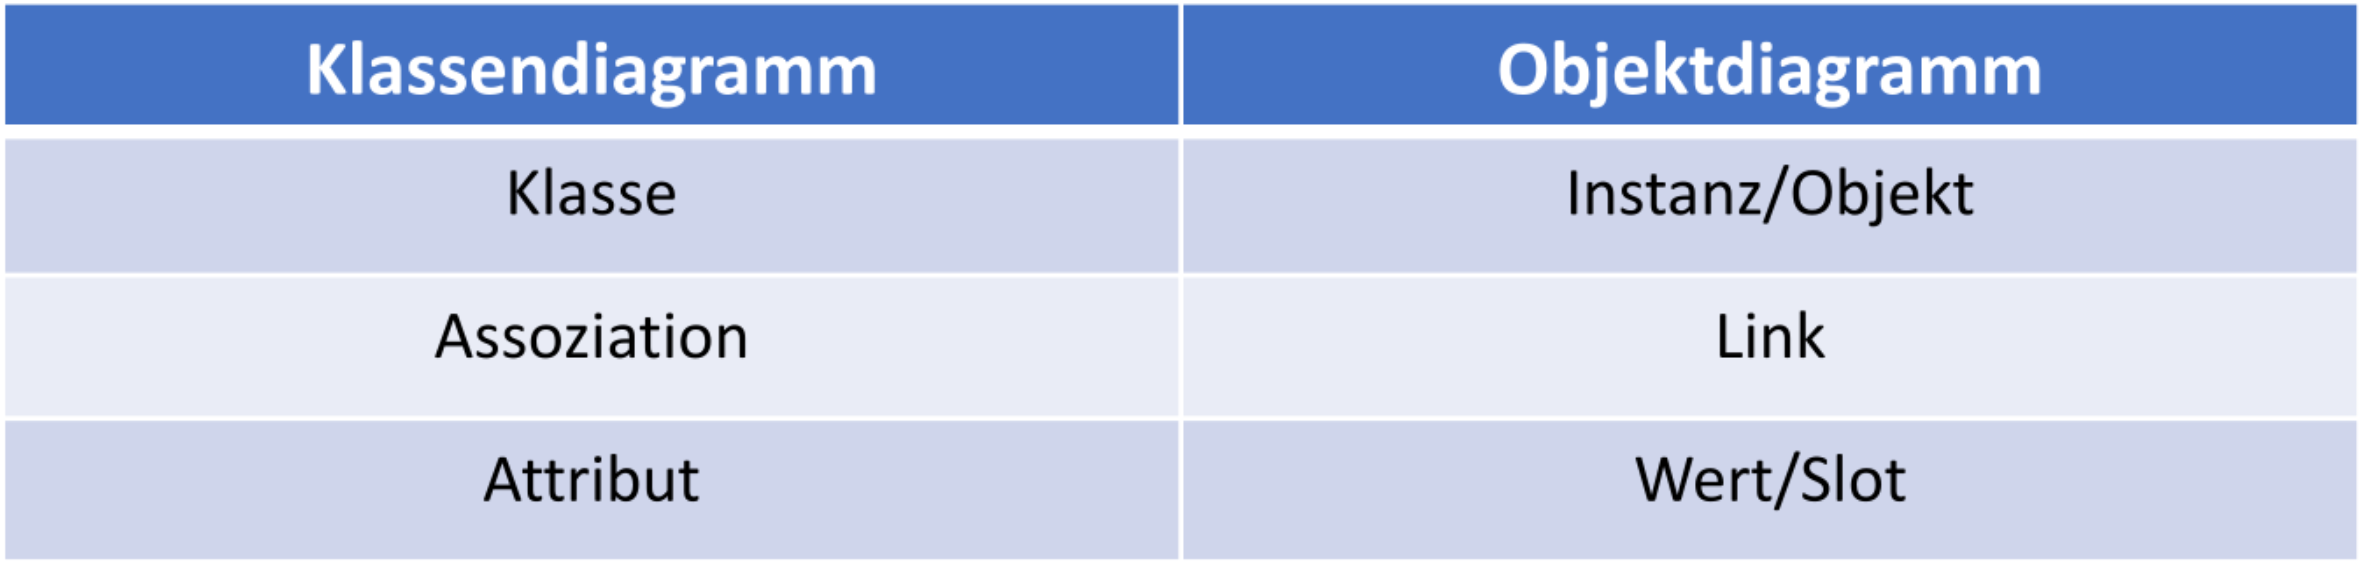
\includegraphics[width=0.95\textwidth]{Objekt-00.png}
\end{minipage}
\begin{minipage}[h]{0.45\textwidth}
    \centering \includegraphics[width=0.95\textwidth]{Objekt-01.png}
\end{minipage}



\raggedright \subsection{Analysemuster}

!!!TODO!!!

\newpage


\raggedright \subsection{Sequenzdiagramme}


\textbf{Sequenzdiagramme liefern eine Antwort auf die Frage:} „Wie läuft die Kommunikation in meinem System ab?“

\vspace{2em}

\centering \includegraphics[width=0.8\textwidth]{Sequenz-00.png}


\raggedright \subsubsection{Methodenaufrufe}

\vspace{1em}

\begin{minipage}[h]{0.4\textwidth}
    \raggedleft \includegraphics[width=1\textwidth]{Sequenz-02.png} 
\end{minipage}
\begin{minipage}[h]{0.55\textwidth}
    \tiny \textbf{Synchroner Aufruf:}
    \begin{itemize}
        \item Empfangendes Objekt verarbeitet die Nachricht und
        \item Liefert anschließend eine Ergebnisantwort zurück
    \end{itemize}
    \vspace{8em}
    \tiny \textbf{Asynchroner Aufruf:}
    \begin{itemize}
        \item Quelle sendet Nachricht an Ziel
        \item Quelle wartet nicht auf Antwort
        \item Sondern fährt mit Verarbeitung fort
    \end{itemize}    
\end{minipage}

\vspace{2em}

\centering \includegraphics[width=0.8\textwidth]{Sequenz-01.png}

\newpage

\raggedright \subsubsection*{Beispiel aus eigenem Projekt}

\centering \includegraphics[width=0.90\textwidth]{Sequenz-03.png}

\vspace{1em}

\raggedright $ \rightarrow $ \textit{Beachte Lebenslinien und lokale Aufrufe!}

\raggedright \subsubsection*{Von Use-Case zu Sequenzdiagramm}

\centering \includegraphics[width=0.90\textwidth]{Sequenz-04.png}

\newpage



\raggedright \subsection{Kommunikationsdiagramme}

\textbf{Kommunikationsdiagramme benatworten die Frage:} \\ “Welche Teile einer komplexen Struktur (aus einem Sequenzdiagramm) arbeiten wie zusammen, um eine bestimmte Funktion zu erfüllen?”

\vspace{1em}

\centering \includegraphics[width=0.75\textwidth]{Kommunikation-00.png}

\vspace{1em}

\raggedright \subsubsection*{Wann verwende ich ein Kommunikationsdiagramm?}

\textbf{Wenn ich eine Interaktion unter folgenden Rahmenbedingungen darstellen möchte:}

\small
\begin{itemize}
    \item Komplexe Struktur mit vielen Teilen, einfaches Zusammenwirken darstellen
    \item Zeitliche Übergänge sind unwichtig
    \item Zustände und Daten sind weniger wichtig
    \item Grundsätzliches Verständnis wichtiger als Details
    \item Einfache Interaktion ohne wichtige zeitliche Abhängigkeiten, Nebenläufigkeiten oder Kontrollelemente
    \item Genau ein Zusammenspiel zeigen, keine Varianten
\end{itemize}

\vspace{1em}

\raggedright \subsubsection*{Anwendungsbeispiel: Suchanfrage}

\centering \includegraphics[width=0.75\textwidth]{Kommunikation-01.png}

\tiny
\begin{itemize}
    \item Nachdem Anwender Suchanfrage formuliert hat, startet er die Suche (1: suchen).
    \item Dann erzeugt die Bedienoberfläche aus der Suchanfrage eine Datenbankabfrage (1.1: erzeuge\_sql-query).
    \item Erzeugte Datenbankanfrage wird gleichzeitig an alle Datenbanken geschickt, die durchsucht werden sollen (1.1.1*||: suche).
    \item Suchergebnisse der Datenbanken werden von der Bedienoberfläche bearbeitet (1.1.1.1: bearbeiten), gesammelt (1.2: sammeln) und dem Anwender präsentiert (1.3: präsentieren).
\end{itemize}

\newpage



\raggedright \subsection{Komponentendiagramme}

\vspace{1em}

\small
\textbf{Kommunikationsdiagramme benatworten die Frage:} \\ „Wie ist mein System strukturiert und wie werden diese Strukturen erzeugt?“

\raggedright \subsubsection{Elemente}

\centering \includegraphics[width=0.9\textwidth]{Komponenten-00.png}

\raggedright \subsubsection*{Beispiel aus eigenem Projekt}

\centering \includegraphics[width=0.9\textwidth]{Komponenten-01.png}

\newpage



\raggedright \subsection{Verteilungsdiagramme}

\vspace{1em}

\textbf{Kommunikationsdiagramme benatworten die Frage:} “Wie werden die Artefakte des Systems zur Laufzeit verteilt?” \\
\tiny \textit{(Verteilung: Installation, Konfiguration, Bereitstellung oder Ausführung)}

\small
\begin{itemize}
    \item Es zeigt die Zuordnung von Artefakten (also u.a. Softwarekomponenten) auf Hardware-Einheiten, die als Knoten bezeichnet werden
    \item Stellt die Kommunikationsverbindungen und Abhängigkeiten zwischen Knoten dar
\end{itemize}

\vspace{2em}

\raggedright \textbf{Grundsätzlich: nur sinnvoll, wenn es auch wirklich etwas zu verteilen gibt}

\textbf{Dann ist es an drei Stellen sinnvoll:}
\begin{itemize}
    \item Systemkontext: “Wie kommuniziert mein System mit Nachbarsystemen”
    \item Design-Phase: “Wie sieht eine Verteilung auf Umgebungen im Prinzip aus?”
    \item Übergabe in den Betrieb: “Wie sieht die konkrete Verteilung aus (Rechnernamen, IP-Adressen, Portnummern, etc.)”
\end{itemize}

\vspace{2em}

\raggedright \subsubsection{Elemente}

\centering \includegraphics[width=0.9\textwidth]{Verteilung-00.png}

\newpage

\begin{minipage}[h]{0.45\textwidth}
    \raggedright \includegraphics[width=0.9\textwidth]{Verteilung-01.png} 
\end{minipage}
\begin{minipage}[h]{0.45\textwidth}
    \raggedleft \includegraphics[width=0.9\textwidth]{Verteilung-02.png}   
\end{minipage}

\vspace{3em}

\begin{minipage}[h]{0.45\textwidth}
    \raggedright \includegraphics[width=0.9\textwidth]{Verteilung-03.png} 
\end{minipage}
\begin{minipage}[h]{0.45\textwidth}
    \raggedleft \includegraphics[width=0.9\textwidth]{Verteilung-04.png}   
\end{minipage}

\vspace{4em}



\subsection{Zusammenfassung der Diagramme}

\centering \includegraphics[width=0.9\textwidth]{UML-01.png}

\newpage

\raggedright \subsubsection*{Welche Fragen beantworten die UML-Diagramme?}
\vspace{3em}
\begin{itemize}
    \item \textbf{Use-Case-Diagramm:}
    \begin{itemize}
        \item „Was leistet mein System für seine Umwelt (Nachbarsysteme, Stakeholder)?“
    \end{itemize}
    \item \textbf{Aktivitätsdiagramm:}
    \begin{itemize}
        \item „Wie läuft ein bestimmter flussorientierter Prozess oder Algorithmus ab?“
    \end{itemize}
    \item \textbf{Zustandsdiagramm:}
    \begin{itemize}
        \item „Welche Zustände kann ein Objekt, eine Schnittstelle, ein Use Case, … bei welchen Ereignissen annehmen?“
    \end{itemize}
    \item \textbf{Klassendiagramm:}
    \begin{itemize}
        \item „Aus welchen Klassen besteht mein System und wie stehen diese untereinander in Beziehung?“
    \end{itemize}
    \item \textbf{Paketdiagramm:}
    \begin{itemize}
        \item „Wie kann ich mein Modell so schneiden, dass ich den Überblick bewahre?“
    \end{itemize}
    \item \textbf{Objektdiagramm:}
    \begin{itemize}
        \item „Welche innere Struktur besitzt mein System zu einem bestimmten Zeitpunkt zur Laufzeit (Klassendiagramm-Schnappschuss)?“
    \end{itemize}
    \item \textbf{Sequenzdiagramm:}
    \begin{itemize}
        \item „Wer tauscht mit wem welche Informationen in welcher Reihenfolge aus?“
    \end{itemize}
    \item \textbf{Kommunikationsdiagramm:}
    \begin{itemize}
        \item „Wer kommuniziert mit wem? Wer ‚arbeitet‘ im System zusammen?“
    \end{itemize}
    \item \textbf{(Timingdiagramm:)}
    \begin{itemize}
        \item „Wann befinden sich verschiedene Interaktionspartner in welchem Zustand?“
    \end{itemize}
    \item \textbf{(Interaktionsübersichtdiagramm:)}
    \begin{itemize}
        \item „Wann läuft welche Interaktion ab?“
    \end{itemize}
    \item \textbf{Komponentendiagramm:}
    \begin{itemize}
        \item „Wie werden meine Klassen zu wiederverwendbaren, verwaltbaren Komponenten zusammengefasst und wie stehen diese miteinander in Beziehung?“
    \end{itemize}
    \item \textbf{Verteilungsdiagramm:}
    \begin{itemize}
        \item „Wie sieht das Einsatzumfeld (Hardware, Server, Datenbanken, …) des Systems aus? Wie werden die Komponenten zur Laufzeit wohin verteilt?“
    \end{itemize}
\end{itemize}



\section{Objektorientiertes Design (OOD)} % --- Objektorientiertes Design (OOD) ------------------------------------------------------------------------------------

\centering \includegraphics[width=0.9\textwidth]{OOD-00.png}


\raggedright \subsection{Designphase}
\begin{itemize}
    \item \textbf{Motivation:} Großprojekte haben oft komplexe Strukturen mit vielen Dialogen und Kernobjekten und erfordern ein großes Team über mehrere Jahre.
    \item \textbf{Ziele der Designphase:} Übergang von den Anforderungen zur Realisierung. Strukturierung und Dekomposition zur Handhabung der Komplexität.
    \item \textbf{Ergebnisse:} Softwarearchitekturmodell, Spezifikation der Systemkomponenten und deren Beziehungen.
\end{itemize}

\subsection{Softwarearchitektur}
\begin{itemize}
    \item \textbf{Korrektheit:} Erfüllung der Anforderungen und Sicherstellung nicht-funktionaler Anforderungen.
    \item \textbf{Wiederverwendung:} Vermeidung von Doppelarbeit zur Erleichterung der Wartung und Weiterentwicklung.
    \item \textbf{Verständlichkeit \& Präzision:} Gute Dokumentation und logische Struktur.
    \item \textbf{Anpassbarkeit:} Einfache Erweiterbarkeit.
\end{itemize}

\begin{itemize}
    \item \textbf{Definition:} Modell eines gesamten Softwaresystems, bestehend aus internen Verhaltenskomponenten und deren Interaktion.
    \item \textbf{Wichtigkeit:} Früheste Designentscheidung, die essenzielle Eigenschaften wie Modifizierbarkeit, Wartbarkeit und Performanz beeinflusst.
\end{itemize}

\newpage

\subsection{Architektursichten}

\subsubsection{4+1 Sichten nach Kruchten}

\centering \includegraphics[width=0.4\textwidth]{Kruchten-00.png}

\begin{itemize}
    \item \textbf{Logische Sicht:}
    \begin{itemize}
        \item \textbf{Adressat:} Endanwender
        \item \textbf{Fokus:} Funktionalität für Endanwender, Funktionale Anforderungen, Dienste, die dem Nutzer bereitgestellt werden
        \item \textbf{Hilfsmittel:} Klassendiagramme, Sequenzdiagramme, Kommunikationsdiagramme
    \end{itemize}
    \item \textbf{Implementierungssicht:}
    \begin{itemize}
        \item \textbf{Adressat:} Entwickler, SW-Manager
        \item \textbf{Fokus:} Systembeschreibung aus Entwicklersicht, Statische Organisation der Software, Software-Management
        \item \textbf{Hilfsmittel:} Komponentendiagramme, Paketdiagramme
    \end{itemize}
    \item \textbf{Prozesssicht:}
    \begin{itemize}
        \item \textbf{Adressat:} Integrierer
        \item \textbf{Fokus:} Dynamische Aspekte des Systems, Nicht-funktionale Anforderungen (Skalierbarkeit, Parallelität, Verteilung, Performanz)
        \item \textbf{Hilfsmittel:} Aktivitätsdiagramme
    \end{itemize}
    \item \textbf{Physische Sicht:}
    \begin{itemize}
        \item \textbf{Adressat:} System-Engineers
        \item \textbf{Fokus:} Nicht-funktionale Anforderungen mit Hinblick auf Hardware (Zuverlässigkeit, Erreichbarkeit, Performanz), Verteilung und Kommunikation der Hardware-Komponenten
        \item \textbf{Hilfsmittel:} Verteilungsdiagramme
    \end{itemize}
    \item \textbf{Szenarien:}
    \begin{itemize}
        \item \textbf{Adressat:} Alle Stakeholder
        \item \textbf{Fokus:} Systemkonsistenz, Ablaufbeschreibung zwischen Komponenten, Architekturüberprüfung
        \item \textbf{Hilfsmittel:} Use-Case-Diagramme, Sequenzdiagramme
    \end{itemize}
\end{itemize}

\newpage


\raggedright \subsubsection{4 Sichten nach Starke}

\centering \includegraphics[width=0.4\textwidth]{Starke-00.png}

\begin{itemize}
    \item \textbf{Kontextsicht:}
    \begin{itemize}
        \item \textbf{Frage:} Wie ist das System in seine Umgebung eingebettet?
        \item \textbf{Beschreibung:} System als Black-Box, Schnittstellen zu Nachbarsystemen, Interaktion mit wichtigen Stakeholdern, wesentliche Teile der Infrastruktur
        \item \textbf{Zweck:} Abstrakte Beschreibung (Vision) des Systems aus der Vogelperspektive
        \item \textbf{UML-Diagramme:} Klassendiagramme (für die Struktur des Systems), Anwendungsfalldiagramme (für Interaktionen mit der Umwelt)
    \end{itemize}
    \item \textbf{Bausteinsicht:}
    \begin{itemize}
        \item \textbf{Frage:} Wie ist das System intern aufgebaut?
        \item \textbf{Beschreibung:} Statische Strukturen des Systems, Subsysteme, Module, Pakete, Komponenten, Klassen etc.
        \item \textbf{Zweck:} Unterstützung bei der Projektüberwachung, Zuteilung von Arbeitspaketen, Referenz für Entwickler
        \item \textbf{UML-Diagramme:} Komponentendiagramme (für die Darstellung von Software-Bausteinen), Klassendiagramme (für die Struktur der Bausteine)
    \end{itemize}
    \item \textbf{Laufzeitsicht:}
    \begin{itemize}
        \item \textbf{Frage:} Wie läuft das System ab?
        \item \textbf{Beschreibung:} Welche Bausteine existieren zur Laufzeit, wie interagieren Bausteine miteinander, dynamische Strukturen
        \item \textbf{Hinweis:} Interessante Laufzeitszenarien, wie z.B. das Starten, Überwachen und Beenden des Systems
        \item \textbf{UML-Diagramme:} Sequenzdiagramme (für Interaktionen zur Laufzeit), Aktivitätsdiagramme (für Abläufe zur Laufzeit), Kommunikationsdiagramme (für die Zusammenarbeit von Objekten)
    \end{itemize}

    \newpage

    \item \textbf{Verteilungssicht:}
    \begin{itemize}
        \item \textbf{Frage:} In welcher Umgebung läuft das System ab?
        \item \textbf{Beschreibung:} Hardwarekomponenten, Netzwerktopologie, Speicher, Router, Firewalls und deren Interaktionen
        \item \textbf{Bedeutung:} Relevant für Betreiber des Systems, Hardware-Architekten, Entwicklungsteam, Management und Projektleitung
        \item \textbf{UML-Diagramme:} Verteilungsdiagramme (für die Zuordnung von Software-Bausteinen zu Hardware-Komponenten)
    \end{itemize}
\end{itemize}

\raggedright \subsubsection{Weitere Sichten}
\begin{itemize}
    \item Szenarien, Datensicht, Sicherheitssicht, QS-Sicht
    \item Nur notwendige Sichten in der erforderlichen Detailtiefe erstellen, um die Komplexität und Pflegeaufwand zu reduzieren
\end{itemize}

\subsubsection{Entwurf von Sichten}
\begin{itemize}
    \item Iterativer Entwurfsprozess aufgrund starker Wechselwirkungen und Abhängigkeiten der Sichten notwendig
    \item Reihenfolge: Kontextsicht, dann Bausteinsicht, Laufzeitsicht oder Verteilungssicht je nach Projektanforderungen
\end{itemize}

\newpage

\subsection{Architekturprinzipien}

\subsubsection{Merkmale schlechter Software}
\begin{itemize}
    \item \textbf{Steif (rigid)}: Schwierige und riskante Änderungen.
    \item \textbf{Zerbrechlich (fragile)}: Fehler in einem Teil verursachen Fehler in anderen.
    \item \textbf{Unbeweglich (immobile)}: Nicht wiederverwendbar, viele Abhängigkeiten.
    \item \textbf{Zäh (viscous)}: Änderungen entgegen dem ursprünglichen Entwurf sind einfacher als konforme Änderungen.
\end{itemize}

\subsubsection{Merkmale guter Software}
\begin{itemize}
    \item \textbf{Einhalten von Prinzipien wie SOLID}:
    \begin{itemize}
        \item \textbf{Single Responsibility Principle}: Jede Klasse hat nur eine Verantwortlichkeit.
        \item \textbf{Open/Closed Principle}: Softwaremodule sollen erweiterbar, aber nicht veränderbar sein.
        \item \textbf{Liskov Substitution Principle}: Objekte der Basisklasse sollten durch Objekte der abgeleiteten Klasse ersetzt werden können, ohne das Verhalten zu ändern.
        \item \textbf{Interface Segregation Principle}: Viele spezifische Schnittstellen sind besser als eine allgemeine.
        \item \textbf{Dependency Inversion Principle}: Abhängigkeiten sollten zu Abstraktionen, nicht zu konkreten Implementierungen bestehen.
    \end{itemize}
\end{itemize}

\subsubsection{Kohäsion}
\begin{itemize}
    \item Kohäsion ist ein Maß für die Zusammengehörigkeit der Bestandteile einer Komponente.
    \item \textbf{Hohe Kohäsion einer Komponente erleichtert}:
    \begin{itemize}
        \item Verständnis
        \item Wartung
        \item Anpassung
    \end{itemize}
    \item \textbf{Hohe Kohäsion wird erreicht durch}:
    \begin{itemize}
        \item Prinzipien der Objektorientierung (Datenkapselung)
        \item Einhaltung von Regeln zur Paketbildung
        \item Verwendung geeigneter Muster zu Kopplung und Entkopplung
    \end{itemize}
\end{itemize}

\newpage

\subsubsection{Kopplung}



\begin{minipage}[h]{0.45\textwidth}
    \centering \includegraphics[width=1\textwidth]{Kopplung-00.JPG}
\end{minipage}
\begin{minipage}[h]{0.45\textwidth}
    \centering \includegraphics[width=1\textwidth]{Kopplung-01.JPG}
\end{minipage}

\raggedright

\begin{itemize}
    \item Kopplung ist ein Maß für die Abhängigkeiten zwischen Komponenten.
    \item \textbf{Geringe Kopplung erleichtert}:
    \begin{itemize}
        \item Wartbarkeit
        \item Stabilität von Systemen
    \end{itemize}
    \item \textbf{Arten der Kopplung}:
    \begin{itemize}
        \item Datenkopplung (gemeinsame Daten)
        \item Schnittstellenkopplung (gegenseitiger Aufruf)
        \item Strukturkopplung (gemeinsame Strukturelemente)
    \end{itemize}
    \item \textbf{Reduktion der Kopplung}:
    \begin{itemize}
        \item Kopplung kann nie auf Null reduziert werden
        \item Schnittstellenkopplung ist akzeptabel, da höhere Flexibilität
        \item Datenkopplung vermeiden (durch Objektorientierung meist gegeben)
        \item Strukturkopplung vermeiden (z.B. keine Vererbung über Paketgrenzen hinweg)
        \item Entkopplungsbeispiel: getter/setter-Methoden statt direkter Attributzugriff
    \end{itemize}
\end{itemize}

\subsubsection{Interne Wiederverwendung}
\begin{itemize}
    \item Interne Wiederverwendung (reuse) ist ein Maß für die Ausnutzung von Gemeinsamkeiten zwischen Komponenten.
    \item \textbf{Ziele der internen Wiederverwendung}:
    \begin{itemize}
        \item Reduktion der Redundanz
        \item Erhöhung der Stabilität und Ergonomie
    \end{itemize}
    \item \textbf{Hilfsmittel für Wiederverwendung}:
    \begin{itemize}
        \item Im objektorientierten Entwurf: Vererbung, Parametrisierung
        \item Im modularen und objektorientierten Entwurf: Module/Objekte mit allgemeinen Schnittstellen (Interfaces)
    \end{itemize}
    \item \textbf{Aber: Wiederverwendung kann die Kopplung erhöhen}:
    \begin{itemize}
        \item Schnittstellenkopplung und Strukturkopplung
    \end{itemize}
\end{itemize}




\subsubsection{DRY-Prinzip}

Don‘t Repeat Yourself

\begin{itemize}
    \item \textbf{Wiederholungen}:
    \begin{itemize}
        \item Machen Arbeit
        \item Werden irgendwann inkonsistent
        \item Erschweren das Verständnis
        \item Verschlechtern Performance beim Kompilieren und zur Laufzeit
    \end{itemize}
    \item \textbf{Vermeide Wiederholungen auf allen Ebenen der Softwareerstellung}:
    \begin{itemize}
        \item Code, Dokumentation, Tests, Datenbankschemata, \dots
    \end{itemize}
\end{itemize}






\raggedright \section{Architekturmuster} % --- Architekturmuster ------------------------------------------------------------------------------------


\subsection{Schichtenarchitektur}

\begin{itemize}
    \item Systeme werden in mehrere logisch zusammengehörige Schichten aufgeteilt.
    \item Jede Schicht stellt Dienstleistungen über Schnittstellen zur Verfügung.
    \item Zugriff nur auf die nächst niedrigere Schicht (strikte Architektur).
\end{itemize}

\subsubsection{Eigenschaften}
\begin{itemize}
    \item Schichten sind nur gekoppelt, wenn sie benachbart sind.
    \item Koppelung auf Schnittstellenebene.
    \item Änderungen wirken sich meist nur lokal aus.
    \item Eine Schicht kann aus mehreren entkoppelten Teilen mit intern hohem Zusammenhalt bestehen.
\end{itemize}

\subsubsection{Vor- und Nachteile}

\textbf{Vorteile}:
\begin{itemize}
    \item Unabhängigkeit der Schichten.
    \item Verteilbar über verschiedene Rechnerknoten.
    \item Minimierte Abhängigkeiten.
\end{itemize}

\textbf{Nachteile}:
\begin{itemize}
    \item Kann die Performance beeinträchtigen.
    \item Schlechte Unterstützung für schichtübergreifende Änderungen.
\end{itemize}


\subsubsection{Die klassische 3-Schichten-Architektur}

\vspace{1em}

\begin{minipage}[h]{0.60\textwidth}
    \tiny
    \begin{enumerate}
        \item[1.] \textbf{Presentation-Layer}
        \begin{itemize}
            \item Realisiert die Benutzeroberfläche.
            \item Stellt Informationen dar und steuert die\\ Benutzerinteraktion.
            \item Greift auf die Application-Layer zu.
            \item Ermöglicht mehrere Oberflächen für dieselbe\\ Applikationslogik.
        \end{itemize}
    \end{enumerate}
\end{minipage}
\begin{minipage}[h]{0.35\textwidth}
    \raggedleft \includegraphics[width=1\textwidth]{Archmuster-00.png}
\end{minipage}

\vspace{1em}

\begin{minipage}[h]{0.45\textwidth}
    \tiny
    \begin{enumerate}
        \item[2.] \textbf{Application-Layer}
        \begin{itemize}
            \item Realisiert die fachliche Funktion der Anwendung.
            \item Kennt keine Informationen über die Presentation-Layer.
            \item Verwaltet Objekte und Klassen des Domänenmodells.
            \item Greift auf Dienste der Persistence-Layer zu.
        \end{itemize}
    \end{enumerate}
\end{minipage}
\begin{minipage}[h]{0.45\textwidth}
    \tiny
    \begin{enumerate}
        \item[3.] \textbf{Persistence-Layer}
        \begin{itemize}
            \item Abstrahiert das Speichermedium von der Applikation.
            \item Speichert Objekte des Domänenmodells persistent ab.
            \item Übersetzt Objekte in ein für die Ablage notwendiges Format.
        \end{itemize}
    \end{enumerate}
\end{minipage}

\vspace{10em}

\subsection{Blackboard-Muster}

\begin{itemize}
    \item Unabhängige Subsysteme, die auf ein gemeinsames Blackboard (Speicher/Datenbank) zugreifen.
    \item Effiziente Methode für gemeinsame Datennutzung.
    \item Schwache Kopplung zwischen Subsystemen.
\end{itemize}

\subsubsection{Vor- und Nachteile}
\textbf{Vorteile}:
\begin{itemize}
    \item Effiziente gemeinsame Datennutzung.
    \item Zentralisierung von Aufgaben wie Datensicherung und Zugriffskontrolle.
\end{itemize}

\textbf{Nachteile}:
\begin{itemize}
    \item Subsysteme müssen dasselbe Datenformat nutzen.
    \item Integration neuer Subsysteme kann schwierig sein.
    \item Blackboard-Komponente als potenzieller Flaschenhals.
\end{itemize}

\newpage

\subsection{Peer-to-Peer}

\vspace{1em}

\begin{minipage}[h]{0.2\textwidth}
    \centering \includegraphics[width=0.75\textwidth]{PtP-00.png} \raggedright
\end{minipage}
\begin{minipage}[h]{0.75\textwidth}
    \begin{itemize}
        \item Gleichberechtigte Komponenten (Peers), die gleichzeitig als Server und Client agieren.
        \item Geeignet für ausfallsichere Datenverteilung wie bei Filesharing oder verteiltem Rechnen.
    \end{itemize}
\end{minipage}





\subsubsection{Vor- und Nachteile}
\textbf{Vorteile}:
\begin{itemize}
    \item Hohe Ausfallsicherheit und Parallelität.
    \item Kein zentraler Flaschenhals.
\end{itemize}

\textbf{Nachteile}:
\begin{itemize}
    \item Auffinden von Peers in großen Netzen kann schwierig sein.
    \item Fehlerbehandlung kann schwierig sein.
\end{itemize}



\subsection{Plug-In-Architektur}

\begin{itemize}
    \item Dynamische Erweiterung des Systems um neue Funktionen ohne Modifikation des Kernsystems.
    \item Externe Module können über Schnittstellen hinzugefügt werden.
\end{itemize}



\subsection{Model View Controller (MVC)}

\begin{itemize}
    \item Aufteilung eines Programms in drei Komponenten:
    \begin{itemize}
        \item Model: Daten und Geschäftslogik.
        \item View: Präsentation und Benutzerinteraktionen.
        \item Controller: Steuerung.
    \end{itemize}
\end{itemize}


\subsection{Thin vs. Fat Client}
\subsubsection{Thin Client}
\begin{itemize}
    \item Nur die Benutzerschnittstelle ist auf dem Client vorhanden.
\end{itemize}

\subsubsection{Fat Client}
\begin{itemize}
    \item Teile oder die gesamte Fachlogik sind auf dem Client.
    \item Entlastung des Servers, aber zusätzliche Anforderungen an die Clients.
\end{itemize}

\vspace{4em}

\raggedright \section{Feindesign und Implementierung} % --- Feindesign und Implementierung ------------------------------------------------------------------------------------

\centering \includegraphics[width=0.9\textwidth]{Feindesign-00.png} 

\centering \includegraphics[width=0.8\textwidth]{Feindesign-01.png}

\vspace{10em}

\raggedright \subsection{Wiederverwendungsebenen}

\begin{itemize}
    \item Nutzung erfolgreicher Entwurfs- und Architekturmuster
    \item Verwendung von Bibliotheken
    \item Verwendung von Frameworks
    \item Wiederverwendung von gesamten Anwendungssystemen
\end{itemize}

\newpage

\raggedright \subsubsection{Vorteile und Kosten}

\begin{itemize}
    \item Vorteile von wiederverwendbaren Systemen:
    \begin{itemize}
        \item Schnellere Entwicklung
        \item Weniger Entwicklungsrisiko
        \item Kostengünstiger
        \item Zuverlässiger (bereits getestet)
    \end{itemize}
    \item Mögliche Kosten:
    \begin{itemize}
        \item Suche und Evaluierung
        \item Kaufkosten
        \item Customizing und Konfiguration
        \item Integration verschiedener Komponenten
    \end{itemize}
\end{itemize}


\raggedright \subsection{Konfigurationsverwaltung}

\begin{itemize}
    \item Grundlegende Aktivitäten:
    \begin{itemize}
        \item Versionsmanagement:
        \begin{itemize}
            \item Verwaltung und Kontrolle verschiedener Versionen der erstellten Artefakte
            \item Koordinierung der Entwicklung von mehreren Programmierern
            \item Verhindert Codeüberschreibungen von unterschiedlichen Programmierern
        \end{itemize}
        \item Systemintegration:
        \begin{itemize}
            \item Unterstützung bei Festlegung, welche Softwareversion welche Komponenten verwendet
            \item Ermöglicht automatisierte Systemerzeugung (Buildsysteme)
        \end{itemize}
        \item Problemverfolgung:
        \begin{itemize}
            \item Tracking von Programmierfehlern und anderen Problemen
            \item Verfolgung, wer welche Probleme löst und wann
        \end{itemize}
    \end{itemize}
\end{itemize}


\raggedright \subsection{Host-Ziel-Entwicklung}

\begin{itemize}
    \item Allgemein:
    \begin{itemize}
        \item Development Platform
        \item Production/Execution Platform
        \item Plattform umfasst mehr als nur Hardware (z.B. OS, DBMS, IDE, ...)
    \end{itemize}
\end{itemize}


\newpage

\section{Design Patterns} % --- Design Patterns ------------------------------------------------------------------------------

Design Patterns sind bewährte, wiederverwendbare Lösungen für häufig auftretende Probleme bei der Softwareentwicklung. Sie bieten eine standardisierte Methode zur Lösung spezifischer Designprobleme, ohne dabei konkrete Implementierungen vorzugeben.

\vspace{2em}

\centering \includegraphics[width=0.75\textwidth]{Designpatterns-00.png}

\raggedright

\vspace{2em}

\section{Template für Design Patterns}
\begin{itemize}
    \item \textbf{Patternname}: Kurzer, beschreibender Name.
    \item \textbf{Motivation}: Grund für das Lernen des Patterns.
    \item \textbf{Zweck}: Beschreibung des Designproblems, das gelöst werden soll.
    \item \textbf{Lösung}: Struktur- und Interaktionsdiagramme.
    \item \textbf{Beispielcode}: Implementierung.
    \item \textbf{Diskussion}: Mögliche Probleme und deren Lösungen.
    \item \textbf{Verwandte Patterns}: Andere relevante Patterns.
\end{itemize}

\newpage

\subsection{Diskussion ausgewählter Design Patterns}

\subsubsection{Singleton}
\begin{itemize}
    \item \textbf{Ziel}: Sicherstellen, dass eine Klasse nur eine Instanz hat.
    \item \textbf{Lösung}: Privater Konstruktor und eine \texttt{getInstance()} Methode.
    \item \textbf{Diskussion}: Performance durch \texttt{synchronized}, Alternativen.
\end{itemize}

\subsubsection{Iterator}
\begin{itemize}
    \item \textbf{Ziel}: Einheitliche Traversierung von Elementen einer Sammlung.
    \item \textbf{Lösung}: Trennung von Iterationslogik und Sammlung.
    \item \textbf{Diskussion}: Verwendung von Interfaces zur Flexibilisierung.
\end{itemize}

\subsubsection{Strategy}
\begin{itemize}
    \item \textbf{Ziel}: Dynamisches Austauschen von Verhalten zur Laufzeit.
    \item \textbf{Lösung}: Abstrakte Strategie-Klasse, konkrete Strategien und eine Kontext-Klasse, die die Strategie hält.
    \item \textbf{Diskussion}: Datentransfer zwischen Context und Strategy, Kopplung reduzieren.
\end{itemize}

\subsubsection{Observer}
\begin{itemize}
    \item \textbf{Ziel}: Benachrichtigung von Objekten bei Zustandsänderungen.
    \item \textbf{Lösung}: Das Subjekt verwaltet eine Liste von Beobachtern und benachrichtigt diese bei Zustandsänderungen.
    \item \textbf{Diskussion}: Lose Kopplung, Push/Pull Benachrichtigungen.
\end{itemize}

\subsubsection{Decorator}
\begin{itemize}
    \item \textbf{Ziel}: Erweiterung des Verhaltens bestehender Klassen zur Laufzeit.
    \item \textbf{Lösung}: Dekorierer-Klassen, die das Verhalten der ursprünglichen Klasse erweitern.
    \item \textbf{Diskussion}: Flexibilität versus Vererbung, Wartbarkeit.
\end{itemize}

\newpage


\section{Factory Pattern} % --- Factory Pattern ---------------------------------------------------------------

\subsection{Fabrikmethode}

Ermöglicht es einer Klasse, die Erstellung von Objekten zu delegieren, ohne die konkrete Implementierung der zu erzeugenden Objekte zu kennen.

\subsubsection*{Vorteile}
\begin{itemize}
    \item Lose Kopplung zwischen Klient und Produkten
    \item Kapselung der Objekterstellung
    \item Trennung von Produkterstellung und -nutzung
\end{itemize}

\subsubsection*{Nachteile}
\begin{itemize}
    \item Erhöhte Komplexität durch Subklassenbildung
    \item Zusätzlicher Programmcode erforderlich
\end{itemize}

\subsection{Abstrakte Fabrik}

Ermöglicht die Erstellung von Objektfamilien, ohne deren konkrete Implementierungen zu kennen.

\subsubsection*{Vorteile}
\begin{itemize}
    \item Kapselung der Objekterstellung
    \item Entkopplung von Klient und konkreten Implementierungen
    \item Einfache Erweiterung um neue Produktfamilien
    \item Konsistente Nutzung von Produktfamilien
\end{itemize}

\subsubsection*{Nachteile}
\begin{itemize}
    \item Hohe Komplexität
    \item Neue Produkte erfordern Änderungen in der gesamten Fabrik-Hierarchie
\end{itemize}


\subsection{Praxisrelevanz}

\vspace{1em}

\begin{minipage}[h]{0.45\textwidth}
    \subsubsection*{Fabrikmethode}
    \begin{itemize}
        \item Häufig verwendet
        \item Reduziert die Komplexität für den Klienten
        \item Erleichtert die Testbarkeit
    \end{itemize}
\end{minipage}
\begin{minipage}[h]{0.45\textwidth}
    \subsubsection*{Abstrakte Fabrik}
    \begin{itemize}
        \item Weniger häufig verwendet
        \item Nützlich in Szenarien mit konsistenten Produktfamilien \\ (z.B. Look and Feel in Benutzeroberflächen)
    \end{itemize}
\end{minipage}

\newpage
 

\section{Testen}

\begin{itemize}
    \item Tests sind notwendig, um sicherzustellen, dass Software korrekt funktioniert und die Anforderungen erfüllt.
    \item Unterscheidung zwischen Verifikation (Überprüfung, ob das Produkt richtig gebaut wurde) und Validierung (Überprüfung, ob das richtige Produkt gebaut wurde).
\end{itemize}

\subsection{Arten von Qualitätssicherungsmaßnahmen}
\begin{itemize}
    \item \textbf{Verifikation:} Formale Beweise der Korrektheit, z.B. mittels Model Checking oder Hoare-Kalkül.
    \item \textbf{Testen:} Durchführung von Tests in verschiedenen Stufen, darunter Modultests, Integrationstests und Abnahmetests.
    \item \textbf{Prüfen:} Menschliche Begutachtung wie Inspektionen, Walkthroughs und Reviews.
\end{itemize}

\subsection{Testphasen}

\subsubsection{Entwicklertests}
\begin{itemize}
    \item Tests, die während der Entwicklung durchgeführt werden, um einzelne Module, Komponenten und das gesamte System zu überprüfen.
    \item \textbf{Modultests:} Testen einzelner Funktionalitäten und Zustände von Objekten.
    \item \textbf{Komponententests:} Fokussieren sich auf die Interaktion zwischen zusammengesetzten Objekten.
    \item \textbf{Systemtests:} Prüfen das Zusammenspiel aller Komponenten.
\end{itemize}

\subsubsection{Freigabetests}
\begin{itemize}
    \item Separates Testteam prüft die vollständige Version des Systems, bevor es an Benutzer freigegeben wird.
    \item Blackbox-Tests und Leistungstests werden durchgeführt.
\end{itemize}

\subsubsection{Benutzertests}
\begin{itemize}
    \item Tests durch die Endbenutzer in ihrer eigenen Umgebung.
    \item Beispiele sind Alphatests (mit Entwicklerunterstützung) und Betatests (unabhängige Tests durch Benutzer).
\end{itemize}

\newpage



\section{Graphen}

Ein Graph \textbf{G = $ (V, V_0, V_f, E) $} ist definiert als:

\begin{itemize}
    \item V = Knotenmenge
    \item $V_0$ = Startknotenmenge
    \item $V_f$ = Endknotenmenge
    \item E = Kantenmenge
\end{itemize}

Die Länge eines Pfades ist die Anzahl der Kanten, aus denen er besteht

\subsection*{SESE-Graphen (Single-Entry, Single-Exit)}

\centering \includegraphics[width=0.75\textwidth]{Graphen-00.png} \raggedright

\subsection*{Testanforderungen (TR)}

Beschreiben Eigenschaften von Testpfaden (z.B. "beinhaltet jeden erreichbaren Knoten von G")

\subsection*{Strukturelle Überdeckungskriterien}

Sind auf einem Graphen lediglich über Knoten und Kanten definiert

Beispiele:

\begin{itemize}
    \item Knotenüberdeckung (NC: node coverage)
    \item Kantenüberdeckung (EC: edge coverage)
    \item Kantenpaar-Überdeckung (EPC: edge-pair coverage)
\end{itemize}

\subsection*{Datenfluss Überdeckungskriterien}

Verlangen, dass ein Graph mit weiteren Informationen (Verweise auf Variablen) angereichert ist

\newpage

\subsection{Knotenüberdeckung (NC)}

Alle erreichbaren Knoten im Graphen müssen besucht werden!

Intuitiv: “jeder Befehl muss ausführbar sein”

\vspace{1em}
\textbf{Beispiel:}

\begin{minipage}[h]{0.3\textwidth}
    \centering \includegraphics[width=0.4\textwidth]{Graphen-01.png} 
\end{minipage}
\begin{minipage}[h]{0.6\textwidth}
    TR = \{ 1, 2, 3 \}, Testpfad = [1, 2, 3]
\end{minipage}


\subsection{Kantenüberdeckung (EC)}

TR enthält jeden erreichbaren Pfad der Länge maximal \textbf{1}, in G!

\vspace{1em}
\textbf{Beispiel:}

\begin{minipage}[h]{0.45\textwidth}
    \centering \includegraphics[width=0.9\textwidth]{Graphen-02.png} \\
    Bemerkung: Testpfad [1,2,3] erfüllt Knotenüberdeckung von G
\end{minipage}
\begin{minipage}[h]{0.45\textwidth}
    \centering \includegraphics[width=0.2\textwidth]{Graphen-03.png} \\
    Auch Graphen erlaubt, die einen Knoten und keine Kanten besitzen!
\end{minipage}


\subsection{Kantenpaar-Überdeckung (EPC)}

TR enthält jeden erreichbaren Pfad der Länge maximal \textbf{2}, in G!

\vspace{1em}
\textbf{Beispiel:}

\includegraphics[width=0.5\textwidth]{Graphen-04.png} \raggedright


\subsection{Vollständige Pfadüberdeckung (CPC)}

TR enthält jeden (erreichbaren) Pfad in G

\newpage

\subsection*{Zusammenfassung \& Beispiel}

\centering \includegraphics[width=0.75\textwidth]{Graphen-05.png} 

\raggedright



\subsection{Einfache Pfade \& Primpfade}\label{subsec:EinfachePfadePrimPfade}

\subsubsection*{Einfache Pfade}

Pfad, auf dem kein Knoten mehrmals vorkommt (Außer erster und letzter Knoten)

\subsubsection*{Primpfade}

Einfacher Pfad, der nicht als echter Teilpfad eines anderen einfachen Pfades auftritt

\vspace{2em}

\textbf{Beispiel:}

\centering \includegraphics[width=0.75\textwidth]{Graphen-06.png} 

\vspace{0.5em}

\tiny \raggedleft $\rightarrow$ \textit{Primpfade ist Teilmenge von Einfache Pfade}

\normalsize

\raggedright

\vspace{2em}

\subsection{Primpfad-Überdeckung (PPC)}

Fordert, dass Zyklen sowohl ausgeführt als auch übersprungen werden können sollen!\\
TR enthält jeden Primpfad in G!

\begin{itemize}
    \item Besuche alle Pfade der Länge 0, 1, 2, 3, ...
    \item Umfasst Knoten- und Kantenüberdeckung
    \item Umfasst fast (aber nicht ganz) EPC
\end{itemize}


\newpage

\subsection{Primpfad Algorithmus}

\vspace{1em}

\begin{enumerate}
    \item Berechne einfache Pfade aufsteigend (Siehe Beispiel \cref{subsec:EinfachePfadePrimPfade})
    \begin{itemize}
        \item Markiere {\color{BrickRed}Rot}: Nicht erweiterbar
        \item Markiere {\color{ForestGreen}Grün}: Zyklus
    \end{itemize}
    \item Alle einfachen, ungefärbten Löschen (Keine Erweiterung möglich)
    \item Teilpfade löschen
\end{enumerate}

$\rightarrow$ Testpfad ermitteln: Nimm längsten Pfand und ergänze alle zum Start \& Ende führenden Knoten




\subsection{Touren}

\vspace{1em}

\centering \includegraphics[width=0.9\textwidth]{Graphen-07.png} 

\raggedright

\newpage

\subsection{Code zu Graph}

\vspace{1em}

Knoten = {\color{BrickRed}Befehle}\\
Kanten = {\color{ForestGreen}Kontrollfluss}

\vspace{1em}

\subsubsection{if-Befehl}

\centering \includegraphics[width=0.9\textwidth]{Graphen-08.png} 

\raggedright

\subsubsection{if-return-Befehl}

\centering \includegraphics[width=0.9\textwidth]{Graphen-09.png} 

\raggedright

\newpage

\subsubsection*{Schleifen}

\vspace{1em}

\begin{itemize}
    \item Bei Schleifen müssen zusätzliche Knoten eingefügt werden
    \item Diese Knoten stellen weder Befehle noch Basisblöcke dar
\end{itemize}

\subsubsection{While}

\centering \includegraphics[width=0.9\textwidth]{Graphen-10.png} 

\raggedright

\subsubsection{For}

\centering \includegraphics[width=0.9\textwidth]{Graphen-11.png} 

\raggedright

\subsubsection{break, continue}

\centering \includegraphics[width=0.9\textwidth]{Graphen-12.png} 

\raggedright

\subsubsection{switch-case}

\centering \includegraphics[width=0.9\textwidth]{Graphen-13.png} 

\raggedright

\newpage

\subsection{Datenfluss-Überdeckungskriterien}

\subsubsection{def \& use}

\begin{itemize}
    \item \textbf{def}: Eine Stelle, an der ein Wert im Speicher gespeichert wird.
    \begin{itemize}
        \item Variable auf der linken Seite einer Zuweisung (z.B. \texttt{x=42}).
        \item Variable ist ein aktueller Parameter in einem Methodenaufruf, der den Wert ändert.
        \item Variable ist ein formaler Parameter einer Methode (implizites \texttt{def} beim Methodenstart).
        \item Variable ist eine Eingabe in ein Programm.
    \end{itemize}
    \item \textbf{use}: Eine Stelle, an der ein Variablenwert genutzt wird.
    \begin{itemize}
        \item Variable auf der rechten Seite einer Zuweisung.
        \item Variable in einer Bedingungsprüfung.
        \item Variable ist ein aktueller Parameter für eine Methode.
        \item Variable ist eine Ausgabe des Programms.
        \item Variable ist eine Ausgabe einer Methode in einer \texttt{return}-Anweisung.
    \end{itemize}
\end{itemize}

$\rightarrow$ Ein DU-Paar (def-use-Paar) liegt nur dann vor, wenn das \texttt{def} nach dem \texttt{use} im gleichen Knoten (Basisblock) auftritt und der Knoten in einer Schleife liegt.

\vspace{1em}

\centering \includegraphics[width=0.9\textwidth]{Graphen-14.png} 

\raggedright

\newpage

\subsection{DU-Touren}

\begin{itemize}
    \item Nutze jedes def (All-Defs-Coverage: ADC)
    \begin{itemize}
        \item $\rightarrow$ Jedes \texttt{def} erreicht \textbf{ein} \texttt{use}
    \end{itemize}
    \item Gelange zu jedem use (All-Uses-Coverage: AUC)
    \begin{itemize}
        \item $\rightarrow$ Jedes \texttt{def} erreicht alle möglichen \texttt{use}
    \end{itemize}
    \item Verfolge alle DU-Pfade (All-DU-Paths-Coverage: ADUPC)
\end{itemize}

\vspace{1em}

\centering \includegraphics[width=0.9\textwidth]{Graphen-15.png} 

\raggedright

\newpage


\section{Vorgehensmodelle}



\subsection{Wasserfall-Modell}

\subsection{V-Modell}

\subsection{Prototypen}

\subsection{Iterative Modelle}

\subsection{Inkrementelle Entwicklung}

\subsection{Iterativ-Inkrementelle Entwicklung (Spiralmodell)}

\subsection{Agile Methoden (Scrum)}

\end{document}